\documentclass[12pt,a4paper]{article}

\usepackage[a4paper,margin=1in]{geometry}
\usepackage{setspace}
\usepackage{titlesec}
\usepackage{graphicx}
\usepackage{longtable}
\usepackage{xcolor}
\usepackage{hyperref}
\usepackage{placeins}
\usepackage{enumitem}
\usepackage{amssymb}

% Compact section spacing
\titlespacing*{\section}{0pt}{12pt plus 4pt minus 2pt}{6pt plus 2pt minus 2pt}
\titlespacing*{\subsection}{0pt}{10pt plus 3pt minus 2pt}{4pt plus 2pt minus 2pt}

\onehalfspacing

\begin{document}

% ==================================================
% COVER PAGE
% ==================================================
\begin{titlepage}
\centering

\vspace*{2cm}

{\Huge \textbf{User Manual}}\\[0.5cm]
{\LARGE \textbf{CodeClash Arena}}\\[2cm]

\textbf{Group Number: XX}\\[0.5cm]
\textbf{Member Names and IDs}\\[3cm]

\textbf{Department of Computer Science and Engineering}\\
\textbf{Military Institute of Science and Technology}\\[1cm]

\textbf{\today}

\vfill
\end{titlepage}

% ==================================================
% TABLE OF CONTENTS
% ==================================================
\tableofcontents
\newpage

% ==================================================
\section{Introduction}

\subsection{Purpose of the Manual}

This user manual serves as a comprehensive guide for users of CodeClash Arena, a gamified competitive programming platform designed to transform traditional coding practice into an interactive and engaging experience. The manual provides detailed instructions on how to use the platform effectively, from account creation to participating in competitive battles and clan wars.

This document is intended for:
\begin{itemize}
\item Beginner programmers seeking to improve their algorithmic skills through competitive practice
\item CSE students looking for engaging coding challenges
\item Competitive programming enthusiasts wanting real-time head-to-head battles
\item Coding instructors and educators implementing gamified learning environments
\item Clan leaders organizing team-based coding competitions
\end{itemize}

The manual covers all essential features of the platform, including step-by-step instructions, visual guidance through screenshots, troubleshooting tips, and best practices for optimal user experience. Whether you are a first-time user or an experienced programmer, this guide will help you navigate the platform efficiently and make the most of its features.

\subsection{Brief Overview of the Web Application}

CodeClash Arena is a web-based competitive programming platform that combines the excitement of multiplayer gaming with professional coding contests. Inspired by popular competitive games like Clash Royale and Clash of Clans, and integrated with the Codeforces problem repository, the platform offers a unique blend of entertainment and skill development.

\subsubsection{Core Concept}

Unlike traditional coding platforms that focus solely on individual practice, CodeClash Arena introduces real-time competitive elements including:
\begin{itemize}
\item \textbf{1v1 Coding Battles}: Challenge other coders in head-to-head real-time competitions
\item \textbf{Clan System}: Form or join teams and participate in clan-based battles
\item \textbf{Rating System}: Track your progress through an ELO-based ranking mechanism
\item \textbf{Practice Gym}: Solo practice mode with access to thousands of programming problems
\item \textbf{Matchmaking}: Automatic pairing with opponents of similar skill levels
\end{itemize}

\subsubsection{Key Differentiators}

CodeClash Arena addresses limitations of conventional coding platforms by providing:
\begin{itemize}
\item Direct head-to-head competition with other coders in real-time
\item Clan-based team competitions fostering collaboration and community
\item Personalized contest creation with custom difficulty and time settings
\item Gamified progression system with levels, XP, and visual achievements
\item Real-time battle synchronization showing opponent progress
\item AI-assisted learning through logical hints during practice sessions
\end{itemize}

\subsubsection{Technical Foundation}

The platform is built using modern web technologies:
\begin{itemize}
\item \textbf{Frontend}: React 19.2.0 with Vite 7.2.4 for fast, responsive user interface
\item \textbf{Backend}: Node.js with Express 4.18.2 for server-side logic
\item \textbf{Database}: Supabase (PostgreSQL) for data management
\item \textbf{Problem Integration}: Codeforces API for accessing thousands of programming problems
\item \textbf{Code Execution}: Piston API for local testing and Codeforces judge for official verdicts
\end{itemize}

\subsubsection{Platform Features Summary}

\begin{longtable}{|p{3.5cm}|p{10cm}|}
\hline
\textbf{Feature} & \textbf{Description} \\
\hline
\endhead

Global Battle Mode & Join a matchmaking queue and compete against players of similar rating in real-time 1v1 battles \\
\hline

Local Battle Mode & Challenge specific friends directly with customizable problem difficulty and time limits \\
\hline

Clan Wars & Form teams, compete in clan-based tournaments, and track team performance \\
\hline

Practice Gym & Access solo practice mode with filtering by difficulty, tags, and rating range \\
\hline

Rating System & ELO-based skill rating that adapts based on opponent strength and battle outcomes \\
\hline

Progression System & Earn experience points and level up through battles and problem solving \\
\hline

Leaderboards & Global and clan rankings updated in real-time showing top performers \\
\hline

Battle History & Comprehensive records of past matches, opponents, and performance metrics \\
\hline

Code Editor & Integrated syntax-highlighted editor supporting C++, Java, Python, JavaScript, and more \\
\hline

AI Hints & Logical approach guidance during practice sessions without revealing solutions \\
\hline

Social Features & Friend lists, clan chat, mail system, and player profile viewing \\
\hline

\end{longtable}

\FloatBarrier

% ==================================================
\section{System Requirements}

This section outlines the technical prerequisites and environmental requirements necessary to access and use CodeClash Arena effectively. Ensuring your system meets these specifications will provide optimal performance and user experience.

\subsection{Supported Browsers and Devices}

\subsubsection{Web Browsers}

CodeClash Arena is a web-based application accessible through modern web browsers. For the best experience, we recommend using the latest stable versions of the following browsers:

\begin{longtable}{|p{3cm}|p{3cm}|p{7.5cm}|}
\hline
\textbf{Browser} & \textbf{Minimum Version} & \textbf{Recommended Features} \\
\hline
\endhead

Google Chrome & Version 84+ & Best performance with V8 JavaScript engine, full CSS Grid and Flexbox gap support, excellent developer tools \\
\hline

Mozilla Firefox & Version 103+ & Strong privacy features, backdrop-filter support, reliable WebSocket connections, modern CSS features \\
\hline

Microsoft Edge & Version 84+ & Chromium-based engine, native Windows integration, excellent performance, full modern CSS support \\
\hline

Safari & Version 15+ & Optimized for macOS/iOS devices, complete modern CSS/JS feature support including aspect-ratio and flex gap \\
\hline

Opera & Version 84+ & Chromium-based, built-in VPN support, efficient resource usage, modern web standards compliance \\
\hline

Brave & Version 1.42+ & Privacy-focused, Chromium-based, full ES2020+ support, modern CSS Grid and Flexbox features \\
\hline

\end{longtable}

\textbf{Important Browser Requirements:}
\begin{itemize}[leftmargin=*]
\item \textbf{JavaScript}: Must be enabled (required for React 19.2.0 and ES2020+ features)
\item \textbf{Cookies}: Must be enabled for session management and authentication
\item \textbf{Local Storage}: Browser must support HTML5 local storage (for user preferences and cached data)
\item \textbf{WebSocket Support}: Required for real-time battle synchronization
\item \textbf{Iframe Support}: Necessary for displaying Codeforces problem statements
\item \textbf{Modern CSS Support}: CSS Grid, Flexbox with gap property, CSS custom properties (variables)
\item \textbf{Advanced CSS Features}: backdrop-filter (with -webkit- prefix for Safari), CSS transforms and transitions
\item \textbf{Modern JavaScript}: ES2020+ features including optional chaining (?.), nullish coalescing (??), async/await
\item \textbf{Pop-up Blocker}: Should allow pop-ups from CodeClash Arena domain for certain features
\end{itemize}

\textbf{Not Recommended or Not Supported:}
\begin{itemize}[leftmargin=*]
\item Internet Explorer (any version) - not supported, lacks modern JavaScript ES6+ features, CSS Grid, and CSS variables
\item Safari versions below 15 - missing critical features like aspect-ratio, full flex gap support, and modern JavaScript operators
\item Firefox versions below 103 - missing backdrop-filter support resulting in visual degradation
\item Chrome/Edge versions below 84 - missing flex gap property causing layout issues
\item Outdated browser versions - may cause compatibility issues, security vulnerabilities, and degraded performance
\item Browsers with JavaScript disabled - critical functionality will not work
\end{itemize}

\subsubsection{Device Compatibility}

CodeClash Arena features a responsive design that adapts to various screen sizes and device types:

\begin{longtable}{|p{3cm}|p{3cm}|p{7.5cm}|}
\hline
\textbf{Device Type} & \textbf{Minimum OS/Browser} & \textbf{User Experience Notes} \\
\hline
\endhead

Desktop Computer & Windows 10+, macOS 11+, Linux & \textbf{Optimal Experience} - Full feature access (1920x1080+ recommended), dual-pane code editor, comfortable coding environment, all modern CSS/JS features supported, best for competitive battles \\
\hline

Laptop & Windows 10+, macOS 11+, Linux & \textbf{Excellent Experience} - All features accessible (1366x768 minimum), suitable for coding and battles, portable competitive environment, modern browser support required \\
\hline

iPad & iOS 15+ with Safari 15+ & \textbf{Good Experience} - 10-inch or larger recommended, touch-optimized interface, suitable for reading problems and light coding, external keyboard strongly recommended for battles, full modern CSS support \\
\hline

Android Tablet & Android 10.0+ with Chrome 84+ & \textbf{Good Experience} - 10-inch or larger recommended, touch-optimized interface, suitable for practice mode, external keyboard recommended, may require Chrome browser installation \\
\hline

iPhone & iOS 15+ with Safari 15+ & \textbf{Limited Experience} - Best for viewing profiles, leaderboards, and battle history; coding on mobile not recommended for competitive battles; requires modern Safari for full feature support \\
\hline

Android Phone & Android 10.0+ with Chrome 84+ & \textbf{Limited Experience} - Best for browsing and monitoring; on-screen keyboard not suitable for competitive coding; install Chrome browser for best compatibility \\
\hline

\end{longtable}

\textbf{Important Device Notes:}
\begin{itemize}[leftmargin=*]
\item \textbf{Older Tablets}: iPads running iOS 14 or Android tablets below version 10.0 may experience visual issues (missing backdrop blur effects, layout problems with flex gap)
\item \textbf{Browser Requirements}: Tablets must use Chrome 84+ (Android) or Safari 15+ (iOS) for full functionality
\item \textbf{Tablet Mode Windows}: Surface devices and 2-in-1 laptops work best in desktop mode with physical keyboard attached
\item \textbf{Mobile Limitations}: While responsive, mobile phones are not recommended for coding battles due to screen size constraints and on-screen keyboard limitations
\item \textbf{Older Devices}: Devices more than 5 years old may struggle with modern JavaScript execution and CSS rendering
\end{itemize}

\textbf{Screen Resolution Recommendations:}
\begin{itemize}[leftmargin=*]
\item \textbf{Minimum}: 1024x768 pixels (basic functionality, some layout compromises on smaller screens)
\item \textbf{Recommended}: 1920x1080 pixels or higher (optimal experience with full CSS Grid layouts)
\item \textbf{Competitive Battle}: 1440x900 pixels minimum (comfortable split-screen view for problem and editor)
\item \textbf{Tablets}: 1280x800 or higher for iPad/Android tablets (portrait mode not recommended for battles)
\item \textbf{Mobile}: 375x667 minimum for basic browsing (coding features disabled on small screens)
\end{itemize}

\textbf{Input Device Recommendations:}
\begin{itemize}[leftmargin=*]
\item \textbf{Physical Keyboard}: Mandatory for competitive battles, required for efficient code input during timed contests
\item \textbf{Mouse/Trackpad}: Strongly recommended for navigation, code selection, and editor interaction
\item \textbf{Touch Screen}: Supported for browsing and navigation but not optimal for code editing; on-screen keyboards significantly slow down coding speed
\item \textbf{Bluetooth Keyboard}: Acceptable for tablets, must support standard keyboard shortcuts (Ctrl+C, Ctrl+V, Tab, etc.)
\item \textbf{External Monitor}: Optional but beneficial for multi-screen setup (problem viewing on one screen, coding on another)
\end{itemize}

\textbf{Tablet-Specific Requirements:}
\begin{itemize}[leftmargin=*]
\item \textbf{iPad Users}: Requires iOS 15+ with Safari 15+, external keyboard mandatory for battles, landscape orientation recommended
\item \textbf{Android Tablet Users}: Requires Android 10.0+ with Chrome 84+ installed, external keyboard strongly recommended
\item \textbf{Stylus Support}: Not utilized by the platform, keyboard input is primary interaction method
\end{itemize}

\subsection{Internet Connection Requirements}

A stable internet connection is essential for CodeClash Arena as it operates entirely online and requires continuous connectivity for real-time features.

\subsubsection{Minimum Internet Speed}

\begin{longtable}{|p{3.5cm}|p{3cm}|p{7cm}|}
\hline
\textbf{Activity} & \textbf{Minimum Speed} & \textbf{Description} \\
\hline
\endhead

General Browsing & 1 Mbps & Basic navigation, viewing profiles, accessing leaderboards \\
\hline

Practice Mode & 2 Mbps & Loading problems, submitting code, receiving verdicts \\
\hline

1v1 Battles & 5 Mbps & Real-time synchronization, live updates, timer synchronization \\
\hline

Clan Wars & 5-10 Mbps & Multiple participants, real-time team coordination \\
\hline

\textbf{Recommended} & \textbf{10 Mbps+} & Optimal performance for all features, minimal latency \\
\hline

\end{longtable}

\subsubsection{Connection Stability}

\begin{itemize}[leftmargin=*]
\item \textbf{Latency}: Less than 200ms ping for optimal real-time battle experience
\item \textbf{Packet Loss}: Less than 1\% for stable WebSocket connections
\item \textbf{Connection Type}: 
  \begin{itemize}
    \item \textbf{Preferred}: Wired Ethernet connection (most stable)
    \item \textbf{Acceptable}: Wi-Fi with strong signal strength (3+ bars)
    \item \textbf{Not Recommended}: Mobile data/cellular (may cause disconnections during battles)
  \end{itemize}
\end{itemize}

\subsubsection{Critical Connectivity Features}

\begin{itemize}[leftmargin=*]
\item \textbf{Real-Time Synchronization}: During battles, the system uses WebSocket connections to synchronize:
  \begin{itemize}
    \item Opponent submission status
    \item Battle timer countdown
    \item Live score updates
    \item Problem acceptance notifications
  \end{itemize}
\item \textbf{External Service Access}: Your network must allow connections to:
  \begin{itemize}
    \item Supabase servers (database and authentication)
    \item Codeforces API endpoints (problem fetching and submission)
    \item Piston API (code execution for practice mode)
    \item Vercel hosting (frontend delivery)
  \end{itemize}
\item \textbf{Firewall Considerations}:
  \begin{itemize}
    \item WebSocket connections (WSS protocol) must not be blocked
    \item HTTPS (port 443) must be accessible
    \item RESTful API calls must be permitted
  \end{itemize}
\end{itemize}

\textbf{Important Note}: Unstable or slow internet connections may result in:
\begin{itemize}[leftmargin=*]
\item Battle disconnections (automatic forfeit if reconnection fails)
\item Delayed submission verdicts
\item Real-time updates lag
\item Timeout errors during code submission
\end{itemize}

\subsection{Required Accounts and Permissions}

\subsubsection{CodeClash Arena Account}

\textbf{Required for}: Access to all platform features

\begin{itemize}[leftmargin=*]
\item \textbf{Registration Information Needed}:
  \begin{itemize}
    \item Valid email address (for account verification and password recovery)
    \item Username (unique identifier, 3-20 characters, alphanumeric)
    \item Strong password (minimum 8 characters, recommended: uppercase, lowercase, numbers, special characters)
  \end{itemize}
\item \textbf{Account Verification}:
  \begin{itemize}
    \item Email verification required upon registration
    \item Verification link expires in 24 hours
    \item Unverified accounts have limited functionality
  \end{itemize}
\item \textbf{Account Permissions}:
  \begin{itemize}
    \item Read access to public leaderboards and profiles
    \item Write access to personal profile information
    \item Participation rights in battles, practice sessions, and clan activities
    \item Submission rights for code solutions
  \end{itemize}
\end{itemize}

\subsubsection{Codeforces Account}

\textbf{Required for}: Code submission and official verdict retrieval\\
\textbf{Requirement Level}: Mandatory for competitive battles and official problem solving

\begin{itemize}[leftmargin=*]
\item \textbf{Why Codeforces Account is Needed}:
  \begin{itemize}
    \item CodeClash Arena integrates with Codeforces for problem sourcing
    \item All code submissions are forwarded to Codeforces judge for verification
    \item Official Codeforces verdicts (Accepted, Wrong Answer, TLE, etc.) are retrieved
    \item Problems are displayed via iframe from Codeforces platform
  \end{itemize}
\item \textbf{Creating a Codeforces Account}:
  \begin{itemize}
    \item Visit \url{https://codeforces.com/register}
    \item Complete registration with email verification
    \item Choose a unique handle (username)
    \item Activate account through confirmation email
  \end{itemize}
\item \textbf{Linking Codeforces Account to CodeClash Arena}:
  \begin{itemize}
    \item Navigate to Profile Settings in CodeClash Arena
    \item Enter your Codeforces handle in the designated field
    \item System validates the handle existence
    \item Handle is stored and used for all future submissions
  \end{itemize}
\item \textbf{Account Permissions Required}:
  \begin{itemize}
    \item Active Codeforces account (not banned or restricted)
    \item Ability to submit solutions to Codeforces problems
    \item Access to Codeforces problem archive
  \end{itemize}
\end{itemize}

\textbf{Important Notes}:
\begin{itemize}[leftmargin=*]
\item Without a linked Codeforces account, users cannot:
  \begin{itemize}
    \item Submit code during battles (automatic forfeit)
    \item Participate in competitive ranked matches
    \item Receive official verdict status
    \item Contribute to clan battle scores
  \end{itemize}
\item Users can still access:
  \begin{itemize}
    \item Platform browsing and exploration
    \item Leaderboard viewing
    \item Profile viewing
    \item Problem browsing (without submission)
  \end{itemize}
\item Codeforces handle cannot be changed frequently (update limit implemented to prevent abuse)
\item Ensure your Codeforces account is in good standing (not restricted for rule violations)
\end{itemize}

\subsubsection{Additional Permissions}

\begin{itemize}[leftmargin=*]
\item \textbf{Browser Permissions}:
  \begin{itemize}
    \item Cookies: Required for session management and authentication persistence
    \item Local Storage: Required for caching user preferences and temporary data
    \item Clipboard Access: Optional, improves code copying experience
  \end{itemize}
\item \textbf{Third-Party Service Access}:
  \begin{itemize}
    \item Supabase (authentication and database): No additional account needed
    \item Piston API (code execution): No additional account needed
    \item Vercel hosting: No user account required
  \end{itemize}
\end{itemize}

\subsection{Software Requirements}

\subsubsection{Operating System Compatibility}

CodeClash Arena is a cross-platform web application compatible with any operating system that supports modern web browsers:

\begin{itemize}[leftmargin=*]
\item \textbf{Windows}: Windows 10 or later (Windows 11 recommended)
\item \textbf{macOS}: macOS 11 (Big Sur) or later (required for Safari 15+)
\item \textbf{Linux}: Any modern distribution (Ubuntu 20.04+, Fedora 33+, etc.)
\item \textbf{Chrome OS}: Latest stable version (Chrome 84+ equivalent)
\item \textbf{iOS}: iOS 15 or later (required for Safari 15+ with full feature support)
\item \textbf{Android}: Android 10.0 or later (for Chrome 84+ support)
\end{itemize}

\subsubsection{No Installation Required}

\begin{itemize}[leftmargin=*]
\item CodeClash Arena is entirely browser-based
\item No desktop application or mobile app download necessary
\item No system administrative privileges required
\item Access the platform directly at: \texttt{[your-deployment-url]}
\end{itemize}

\subsubsection{Optional Enhancements}

\begin{itemize}[leftmargin=*]
\item \textbf{Code Editor Extensions}: While the platform provides an integrated code editor, advanced users may prefer:
  \begin{itemize}
    \item Copying code to external IDEs (VS Code, Sublime Text) for complex solutions
    \item Using browser extensions for enhanced syntax highlighting
  \end{itemize}
\item \textbf{Screen Management}: For optimal battle experience:
  \begin{itemize}
    \item Multiple monitor setup (problem on one screen, editor on another)
    \item Split-screen window management
    \item Browser tab management for simultaneous problem viewing
  \end{itemize}
\end{itemize}

\subsection{Hardware Recommendations}

\begin{longtable}{|p{3cm}|p{3cm}|p{3cm}|p{4.5cm}|}
\hline
\textbf{Component} & \textbf{Minimum} & \textbf{Recommended} & \textbf{Purpose} \\
\hline
\endhead

Processor & Dual-core 2.0 GHz & Quad-core 2.5 GHz+ & Fast page rendering, smooth real-time updates \\
\hline

RAM & 4 GB & 8 GB or more & Multiple browser tabs, smooth multitasking \\
\hline

Storage & N/A (web-based) & N/A & No local installation required \\
\hline

Display & 1024x768 resolution & 1920x1080 or higher & Comfortable coding environment, split-screen view \\
\hline

\end{longtable}

\subsection{Network Security Considerations}

\begin{itemize}[leftmargin=*]
\item \textbf{Corporate Networks}: Some corporate firewalls may block:
  \begin{itemize}
    \item WebSocket connections (required for real-time battles)
    \item External API calls (Codeforces, Piston API)
    \item Iframe embedding (problem display)
  \end{itemize}
  \textit{Solution}: Contact your network administrator to whitelist necessary domains
\item \textbf{VPN Users}: VPN connections may introduce latency affecting real-time battle performance
\item \textbf{Proxy Servers}: Ensure proxy configuration allows WebSocket (WSS) connections
\end{itemize}

\subsection{Accessibility Requirements}

\begin{itemize}[leftmargin=*]
\item \textbf{Visual}: Minimum 768px width viewport for usable interface
\item \textbf{Color Scheme}: System adapts to different lighting conditions; custom themes may be implemented in future versions
\item \textbf{Font Rendering}: Browser must support standard web fonts for proper code editor display
\end{itemize}

\subsection{Modern Web Features and Browser Compatibility}

CodeClash Arena utilizes cutting-edge web technologies that require modern browser support. The following features are implemented:

\begin{itemize}[leftmargin=*]
\item \textbf{CSS Features}: Grid Layout, Flexbox with gap property, CSS Custom Properties (variables), backdrop-filter for blur effects, transforms and transitions
\item \textbf{JavaScript Features}: ES2020+ syntax including optional chaining (?.), nullish coalescing (??), async/await, arrow functions, destructuring, template literals
\item \textbf{Web APIs}: WebSocket (real-time communication), Fetch API (HTTP requests), Local Storage API, History API (routing), Clipboard API
\item \textbf{React 19.2.0}: Modern Hooks (useState, useEffect, useContext), latest rendering optimizations
\end{itemize}

\textbf{Minimum Browser Versions for Full Compatibility:}
\begin{itemize}[leftmargin=*]
\item Chrome/Edge 84+ (for Flexbox gap support)
\item Firefox 103+ (for backdrop-filter support)
\item Safari 15+ (for complete modern CSS/JS features)
\item Mobile Safari iOS 15+ (for full mobile compatibility)
\end{itemize}

\subsection{System Requirements Summary}

\begin{center}
\begin{tabular}{|p{7cm}|p{7cm}|}
\hline
\textbf{Requirement Category} & \textbf{Status} \\
\hline
Modern Web Browser (Chrome 84+, Firefox 103+, Edge 84+, Safari 15+) & \textcolor{red}{MANDATORY} \\
\hline
JavaScript Enabled (ES2020+ support) & \textcolor{red}{MANDATORY} \\
\hline
Modern CSS Support (Grid, Flexbox gap, backdrop-filter) & \textcolor{red}{MANDATORY} \\
\hline
Internet Connection (5+ Mbps recommended) & \textcolor{red}{MANDATORY} \\
\hline
CodeClash Arena Account & \textcolor{red}{MANDATORY} \\
\hline
Codeforces Account (linked handle) & \textcolor{red}{MANDATORY} \\
\hline
Desktop/Laptop Device (for competitive battles) & \textcolor{red}{MANDATORY} \\
\hline
Physical Keyboard (for competitive battles) & \textcolor{red}{MANDATORY} \\
\hline
Stable Internet (Wired connection preferred) & \textbf{RECOMMENDED} \\
\hline
\end{tabular}
\end{center}

\textbf{Note}: Mobile devices (tablets, phones) can be used for browsing profiles, viewing leaderboards, and monitoring battles, but Desktop/Laptop with Physical Keyboard is mandatory for participating in competitive coding battles.

\FloatBarrier

% ==================================================
\section{Getting Started}

This section provides step-by-step instructions for new users to access CodeClash Arena, create an account, log in, and navigate the initial setup process.

\subsection{Accessing the Platform}

CodeClash Arena is accessible through any modern web browser without requiring software installation.

\textbf{Steps to Access:}
\begin{enumerate}
\item Open your preferred web browser (Chrome 84+, Firefox 103+, Edge 84+, or Safari 15+)
\item Navigate to the CodeClash Arena URL: \url{https://code-clash-arena-six.vercel.app/}
\item Ensure JavaScript is enabled in your browser settings
\item The homepage will load, displaying the main landing page
\end{enumerate}

\textbf{First-Time Visitors:} Upon accessing the platform for the first time, you will see the homepage featuring:
\begin{itemize}[leftmargin=*]
\item Main title: "HELLO CODERS, WELCOME!"
\item \textbf{GET STARTED} button - Click to proceed to the Login page
\item \textbf{About us} link in the header - Learn about the platform
\item \textbf{Learn More} link in the header - Discover features and capabilities
\item Animated particle effects for visual engagement
\end{itemize}

\subsection{Sign-Up Process}

New users must create a CodeClash Arena account to access platform features. The sign-up process is straightforward and requires basic information.

\subsubsection{Sign-Up Steps}

\textbf{Step 1: Navigate to Sign-Up Page}
\begin{itemize}[leftmargin=*]
\item From the homepage, click the \textbf{"GET STARTED"} button
\item You will be redirected to the Login page first
\item On the Login page, locate the text at the bottom: \textbf{"Don't have an account?"}
\item Click the \textbf{"Sign Up"} link (highlighted in gold/yellow color)
\item The Sign-Up page will load with registration form
\end{itemize}

\begin{figure}[!htb]
\centering
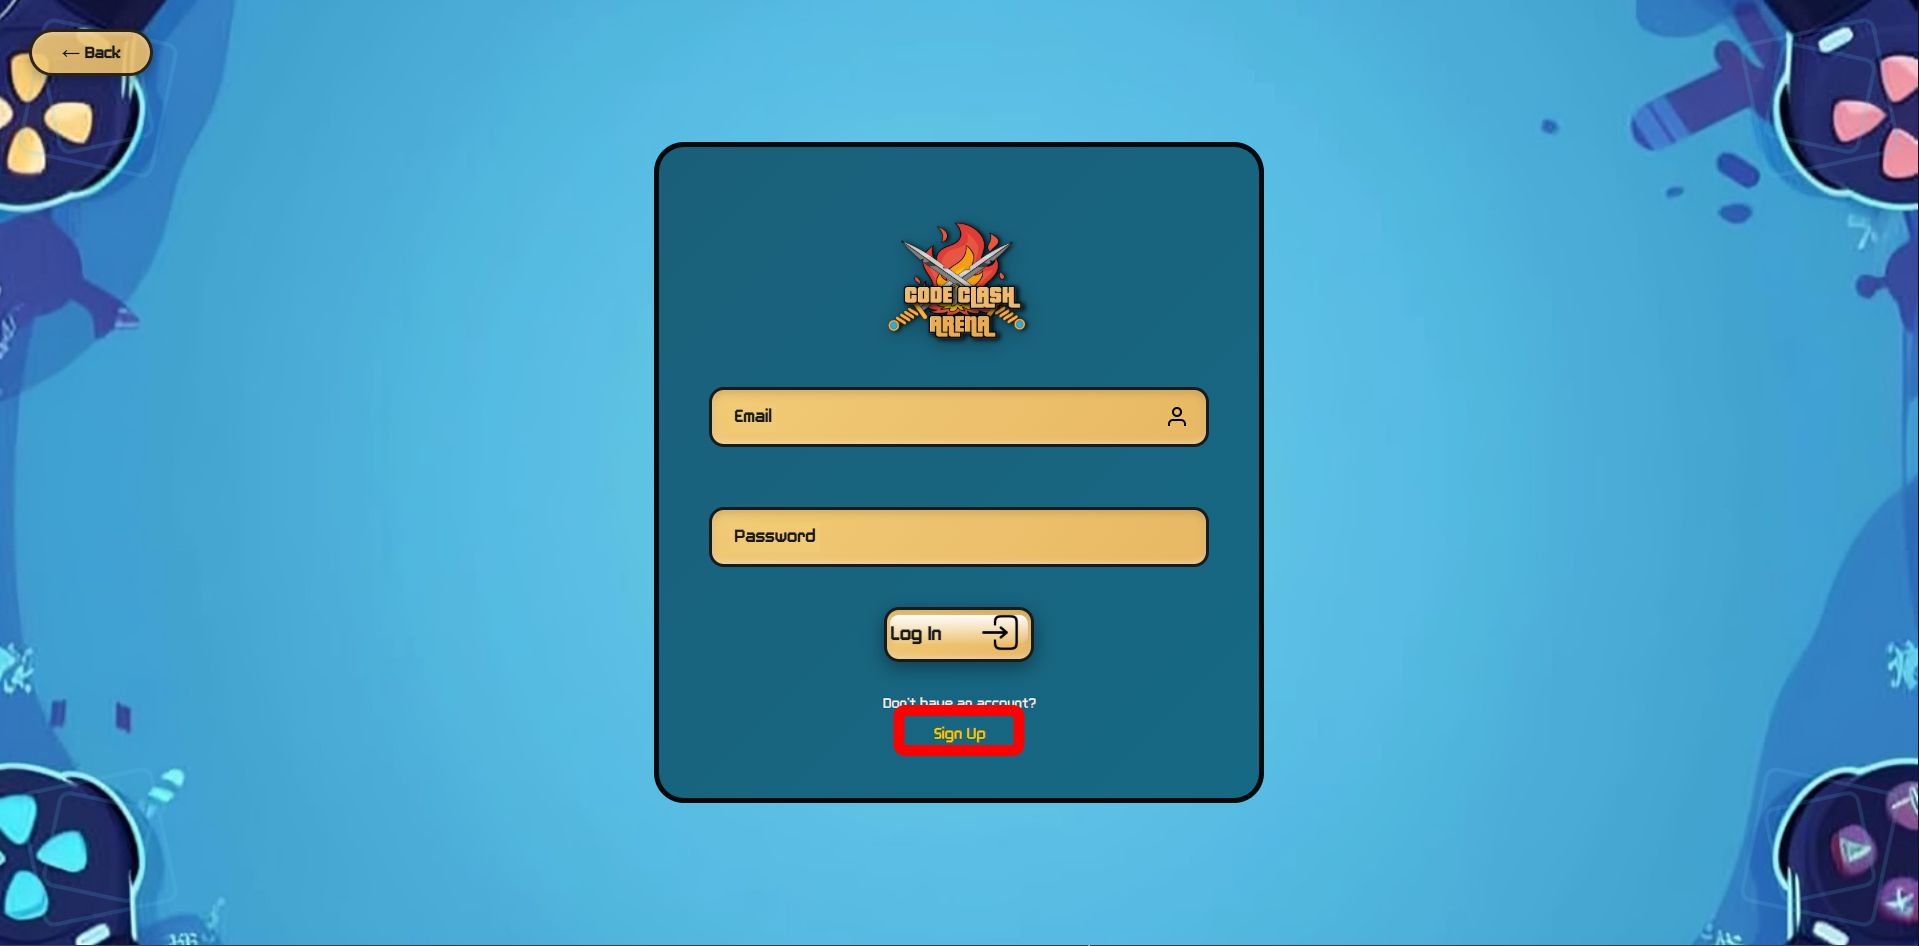
\includegraphics[width=0.95\textwidth]{homepage.png}
\caption{CodeClash Arena Loginpage - Locate Sign Up button}
\label{fig:homepage}
\end{figure}

\textbf{Step 2: Enter Registration Information}

Fill in all three required fields in the sign-up form:

\begin{itemize}[leftmargin=*]
\item \textbf{Email}: Provide a valid email address
  \begin{itemize}
    \item Used for account verification and password recovery
    \item Must be unique (not already registered in the system)
    \item Ensure you have access to this email for verification
    \item Format: username@domain.com
  \end{itemize}
\item \textbf{Codeforces Handle}: Enter your existing Codeforces username
  \begin{itemize}
    \item \textbf{This is your Codeforces account username} - not a new username
    \item Must be a valid, existing Codeforces handle
    \item This handle is linked immediately during registration
    \item Used for all code submissions and battle participation
    \item If you don't have a Codeforces account, create one first at \url{https://codeforces.com/register}
  \end{itemize}
\item \textbf{Password}: Create a strong password for your CodeClash Arena account
  \begin{itemize}
    \item Minimum 8 characters required
    \item Recommended: Include uppercase, lowercase, numbers, and special characters
    \item Password is case-sensitive
    \item This is separate from your Codeforces password
  \end{itemize}
\end{itemize}

\textbf{Important Note:} Unlike typical registrations, CodeClash Arena requires your Codeforces handle during sign-up because the platform integrates directly with Codeforces for problem sourcing and code submission.

\begin{figure}[!htb]
\centering
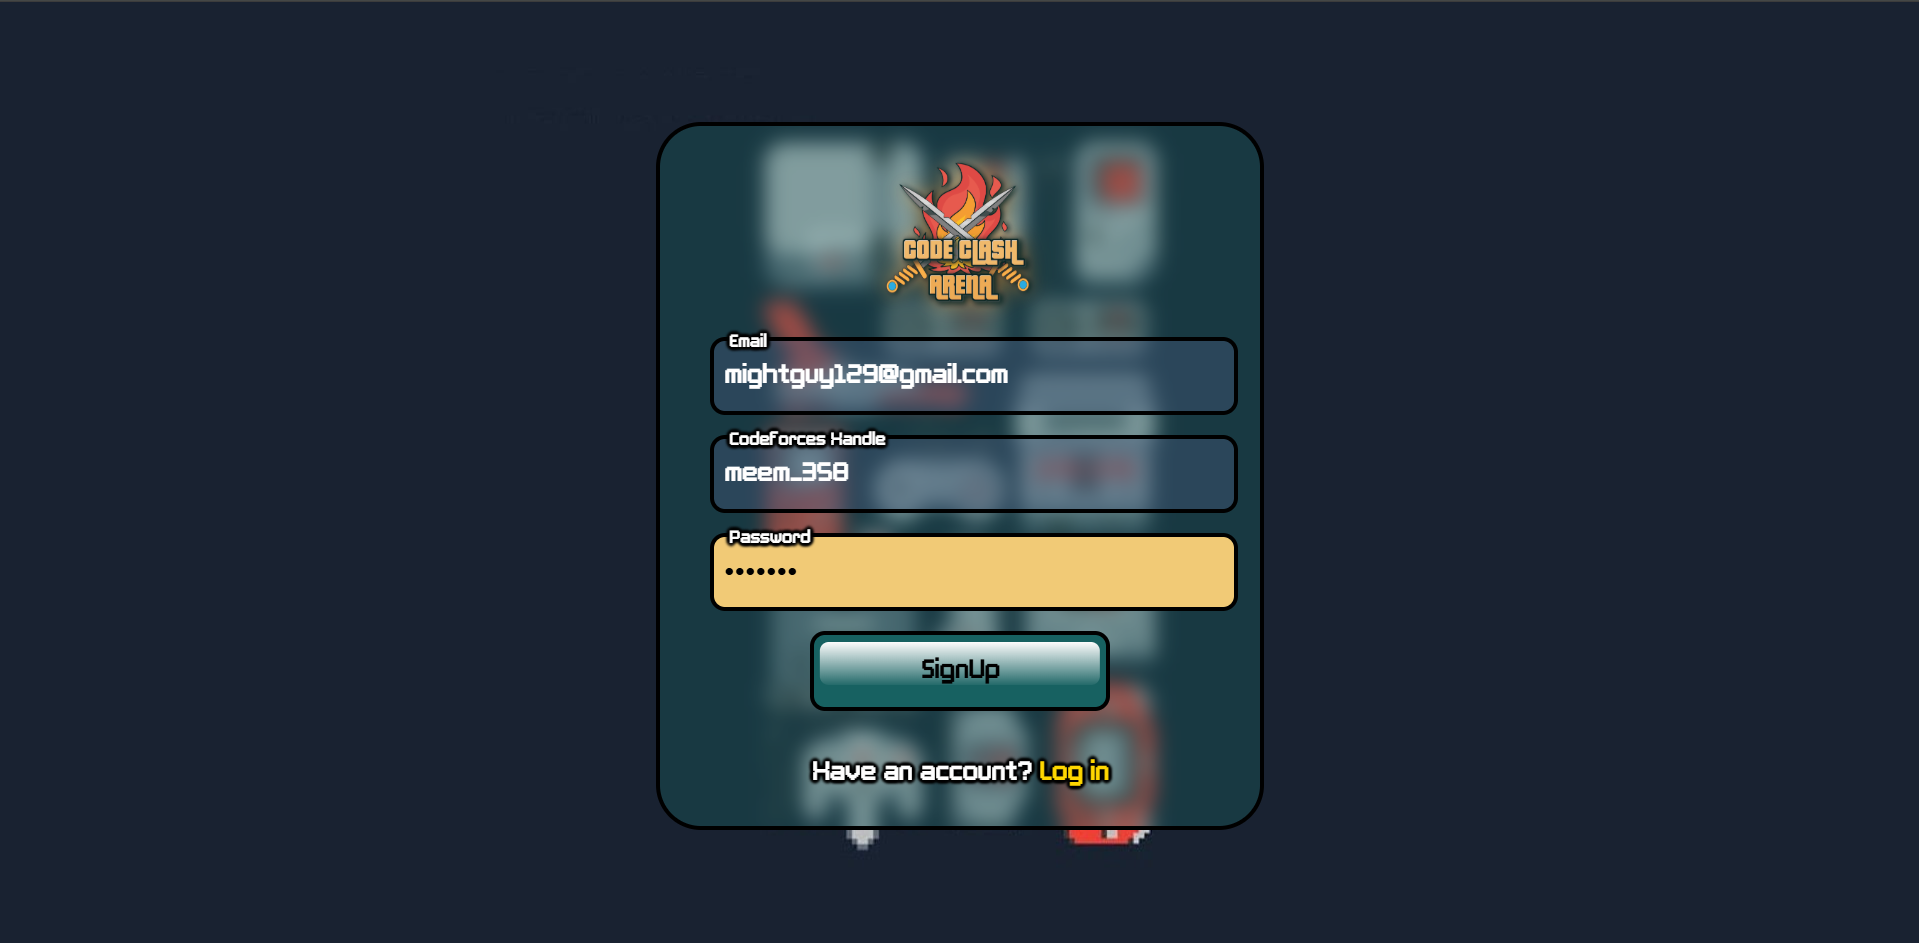
\includegraphics[width=0.9\textwidth]{signup_form.png}
\caption{Sign-Up Form - Enter registration details}
\label{fig:signup_form}
\end{figure}

\textbf{Step 3: Submit Registration}

\begin{itemize}[leftmargin=*]
\item Click the \textbf{"SignUp"} button (green/teal colored button)
\item The system will validate all entered information
\item If validation fails, field labels will turn red indicating errors:
  \begin{itemize}
    \item Red label on Email - Check email format or email may already be registered
    \item Red label on Codeforces Handle - Verify handle exists on Codeforces
    \item Red label on Password - Ensure password meets minimum requirements (8+ characters)
    \item Empty fields are highlighted in red when attempting to submit
  \end{itemize}
\item Upon successful validation, account creation begins
\end{itemize}

\begin{figure}[!htb]
\centering
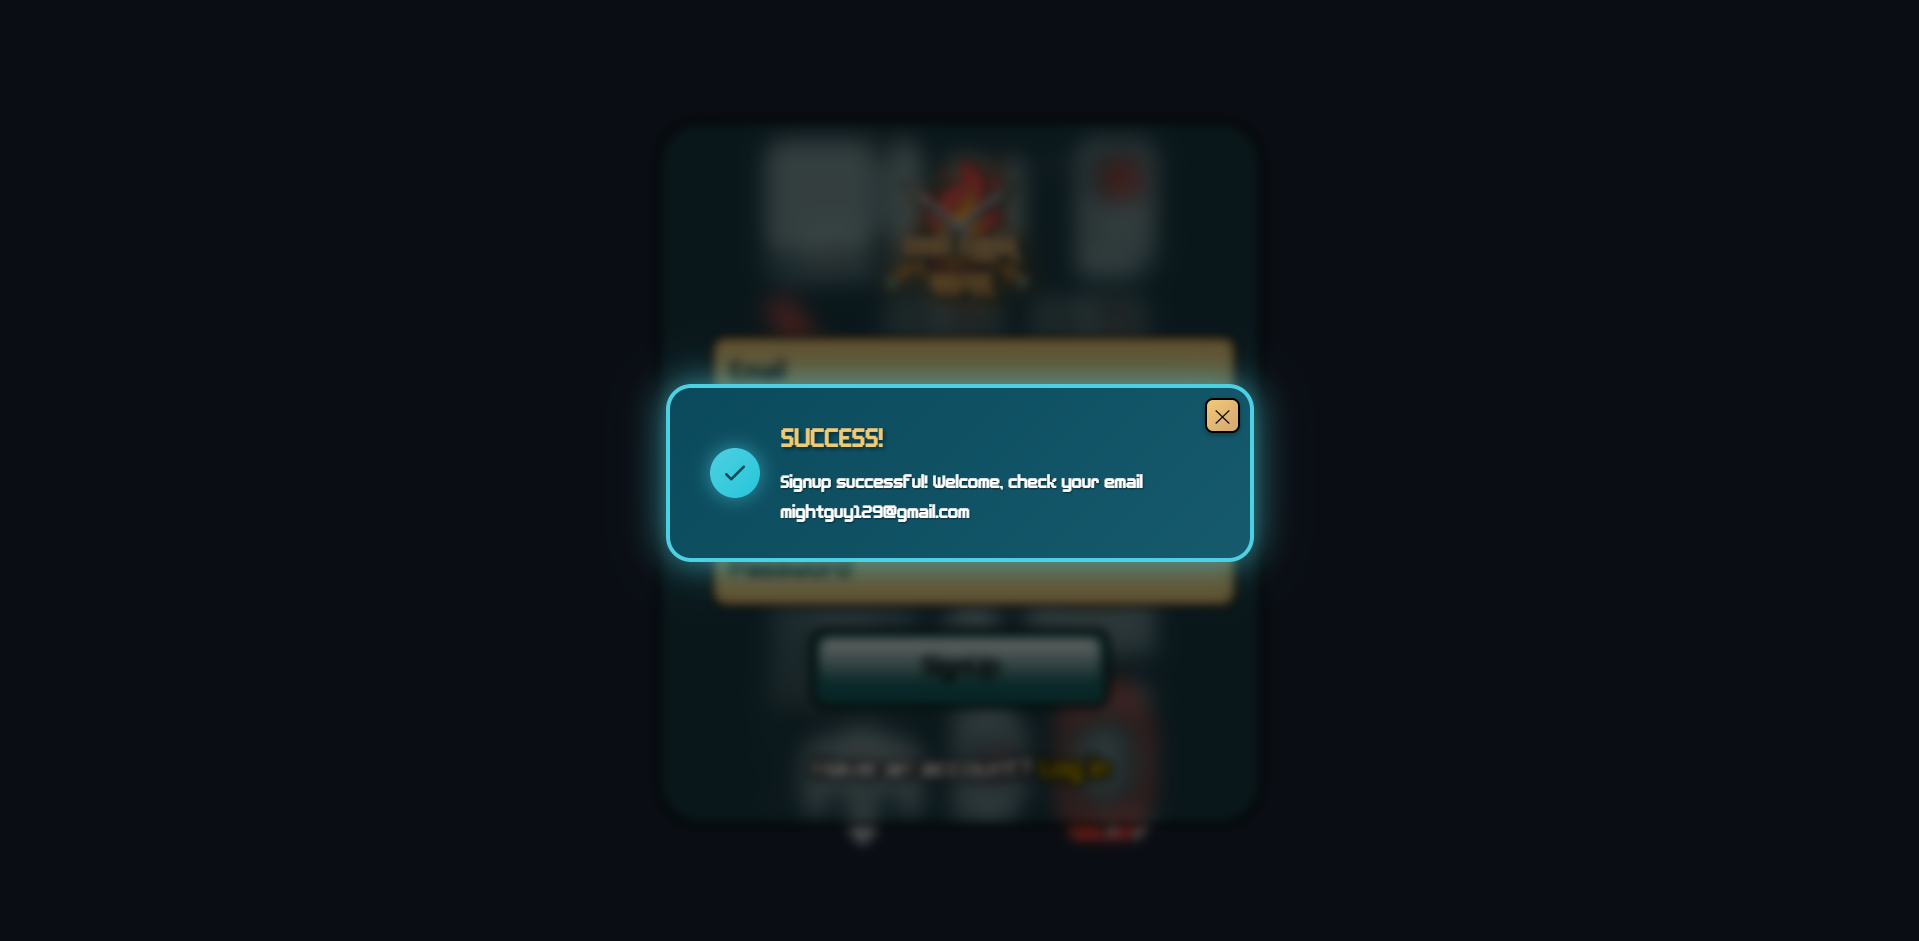
\includegraphics[width=0.9\textwidth]{signup_submit.png}
\caption{Sign-Up Form Completion - Click SignUp button}
\label{fig:signup_submit}
\end{figure}

\textbf{Step 4: Email Verification Alert}

\begin{itemize}[leftmargin=*]
\item After successful registration, a success alert popup appears with the message: \textbf{"Signup successful! Welcome, check your email [your-email@domain.com]"}
\item The page automatically redirects to the Homepage after 1.5 seconds
\item Check your email inbox for a verification message from Supabase (CodeClash Arena's authentication provider)
\item Subject line typically: "Confirm Your Email" or "Verify Your Email"
\item Email may take 1-5 minutes to arrive
\item Check spam/junk folder if email is not received within 5 minutes
\end{itemize}

\begin{figure}[!htb]
\centering
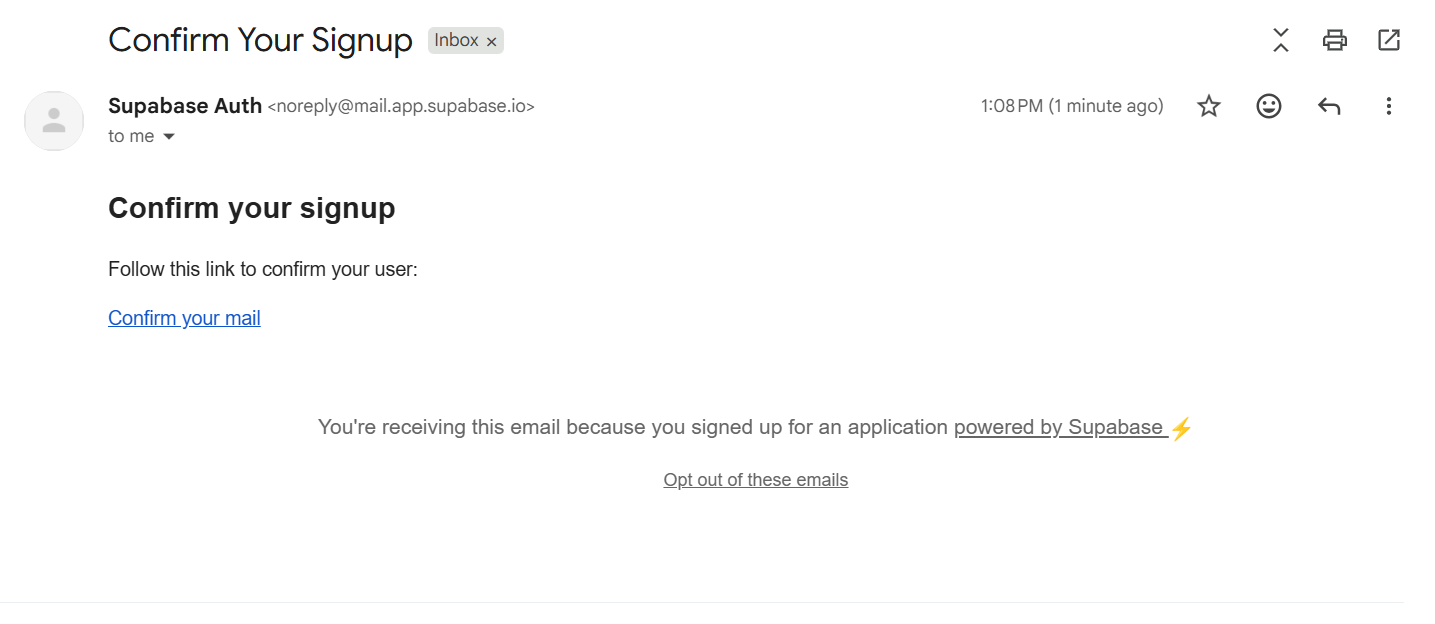
\includegraphics[width=0.9\textwidth]{verification_email.png}
\caption{Email Verification }
\label{fig:verification_prompt}
\end{figure}

\textbf{Step 5: Verify Email Address}

\begin{itemize}[leftmargin=*]
\item Open the verification email
\item Click on the \textbf{"Verify Email Address"} button or link
\item Browser will open and redirect to CodeClash Arena
\item Verification confirmation page appears
\item Account is now fully activated
\end{itemize}

\textbf{Step 6: Login to Complete Setup}

After email verification:
\begin{itemize}[leftmargin=*]
\item Navigate to the Login page
\item Login using your registered email and password
\item Your Codeforces handle is already linked from registration
\item You can now access all platform features including battles, practice gym, and clan wars
\end{itemize}

\textbf{Important Notes:}
\begin{itemize}[leftmargin=*]
\item \textbf{Codeforces Handle Required First}: You must have an existing Codeforces account before signing up on CodeClash Arena
\item \textbf{Verification Link Expiry}: Email verification links typically expire after 24 hours
\item \textbf{Unverified Accounts}: You must verify your email to login and access platform features
\item \textbf{Handle Validation}: The system stores your Codeforces handle but doesn't validate its existence during registration - ensure you enter it correctly
\item \textbf{Account Security}: Never share your CodeClash Arena password with anyone (keep it separate from your Codeforces password)
\item \textbf{Success Alert}: Green alert popup confirms successful registration
\item \textbf{Error Alert}: Red alert popup displays error messages if registration fails
\end{itemize}

\FloatBarrier

\subsection{Login Process}

Existing users can access their accounts through the login page. The process is quick and secure.

\subsubsection{Login Steps}

\textbf{Step 1: Navigate to Login Page}

\begin{itemize}[leftmargin=*]
\item From the homepage, click the \textbf{"GET STARTED"} button
\item You will be automatically redirected to the Login page
\item Alternatively, navigate directly via your browser if you know the URL
\item The login page displays with the CodeClash Arena logo at the top
\item A \textbf{"← Back"} button is available in the top-left corner to return to the homepage
\end{itemize}

\begin{figure}[!htb]
\centering
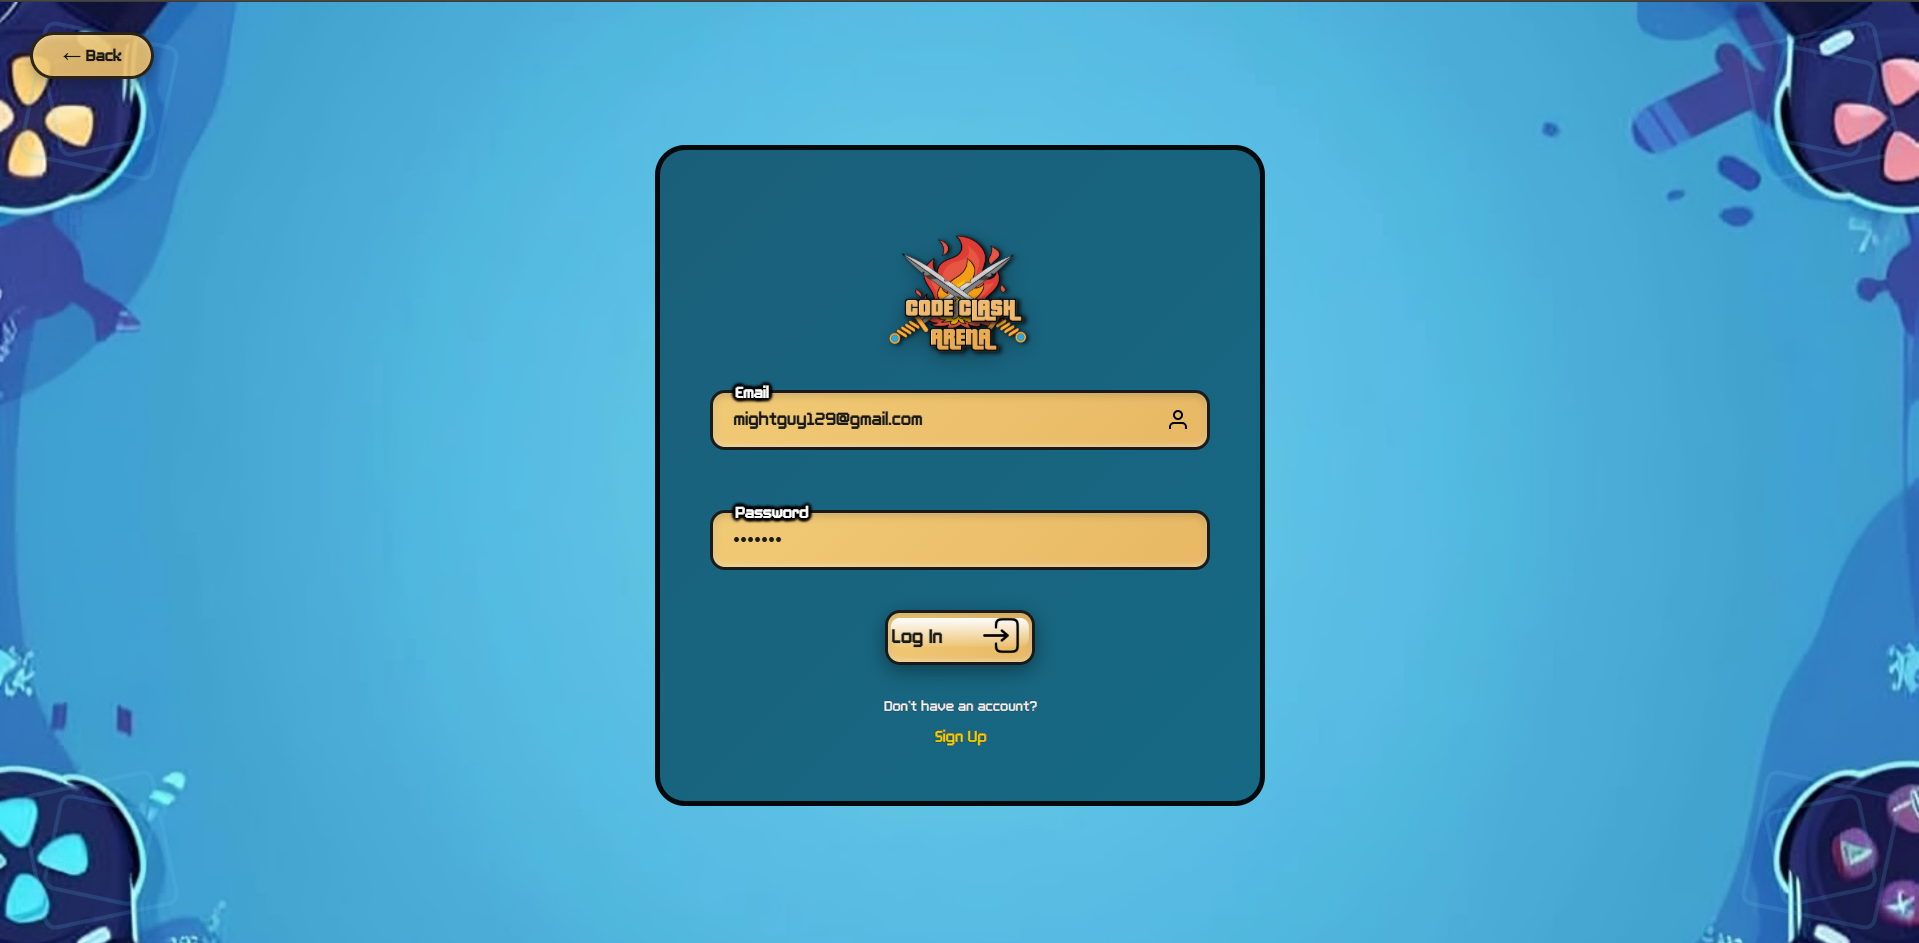
\includegraphics[width=0.95\textwidth]{loginpage.png}
\caption{Loginpage - Navigate to Login}
\label{fig:homepage_login}
\end{figure}

\textbf{Step 2: Enter Login Credentials}

\begin{itemize}[leftmargin=*]
\item \textbf{Email Field}: Enter the email address used during registration
  \begin{itemize}
    \item Labeled as "Email" with a user icon on the left
    \item Email is case-insensitive
    \item Ensure no extra spaces before or after email
    \item Floating label design - label moves up when you start typing
  \end{itemize}
\item \textbf{Password Field}: Enter your account password
  \begin{itemize}
    \item Labeled as "Password" with floating label design
    \item Password is case-sensitive
    \item Click on the password field to focus it
    \item When focused, an \textbf{eye icon} appears on the right side
    \item Click the eye icon to toggle password visibility (show/hide)
    \item Closed eye icon = password hidden; Open eye icon = password visible
  \end{itemize}
\end{itemize}

\textbf{Step 3: Submit Login}

\begin{itemize}[leftmargin=*]
\item Click the \textbf{"Log In"} button (golden/yellow colored button with login icon)
\item System validates credentials with Supabase authentication service
\item Authentication typically completes within 1-2 seconds
\item Success or error alert popup will appear
\end{itemize}

\begin{figure}[!htb]
\centering
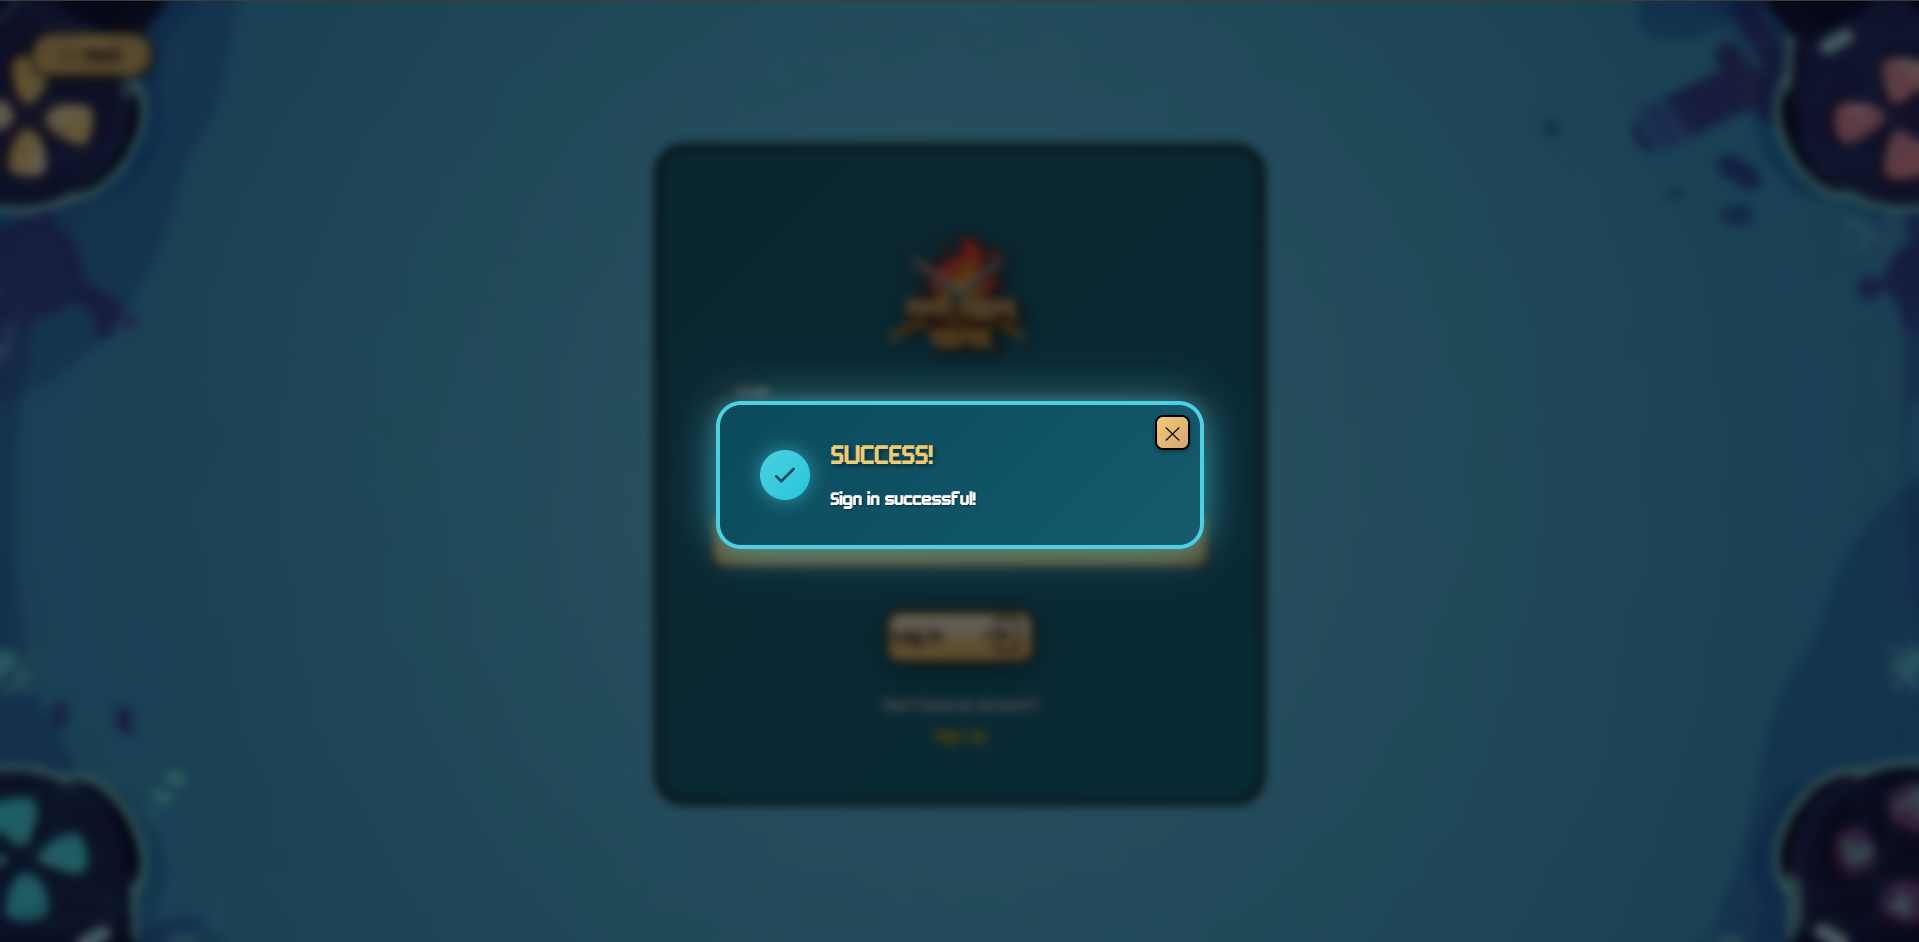
\includegraphics[width=0.9\textwidth]{login_submit.png}
\caption{Login successful - Success alert displayed}
\label{fig:login_success}
\end{figure}

\textbf{Step 4: Successful Login - Redirection}

\begin{itemize}[leftmargin=*]
\item Upon successful authentication, a green success alert appears: \textbf{"Sign in successful!"}
\item After 1.5 seconds, you are automatically redirected to the \textbf{Main Dashboard} (/main)
\item Your Codeforces handle is automatically loaded from the database and stored in browser localStorage
\item Navigation bar updates to show logged-in status with your profile information
\item Access to all platform features is now available: PvP Battles, Practice Gym, Clan Wars, Leaderboards
\end{itemize}

\begin{figure}[!htb]
\centering
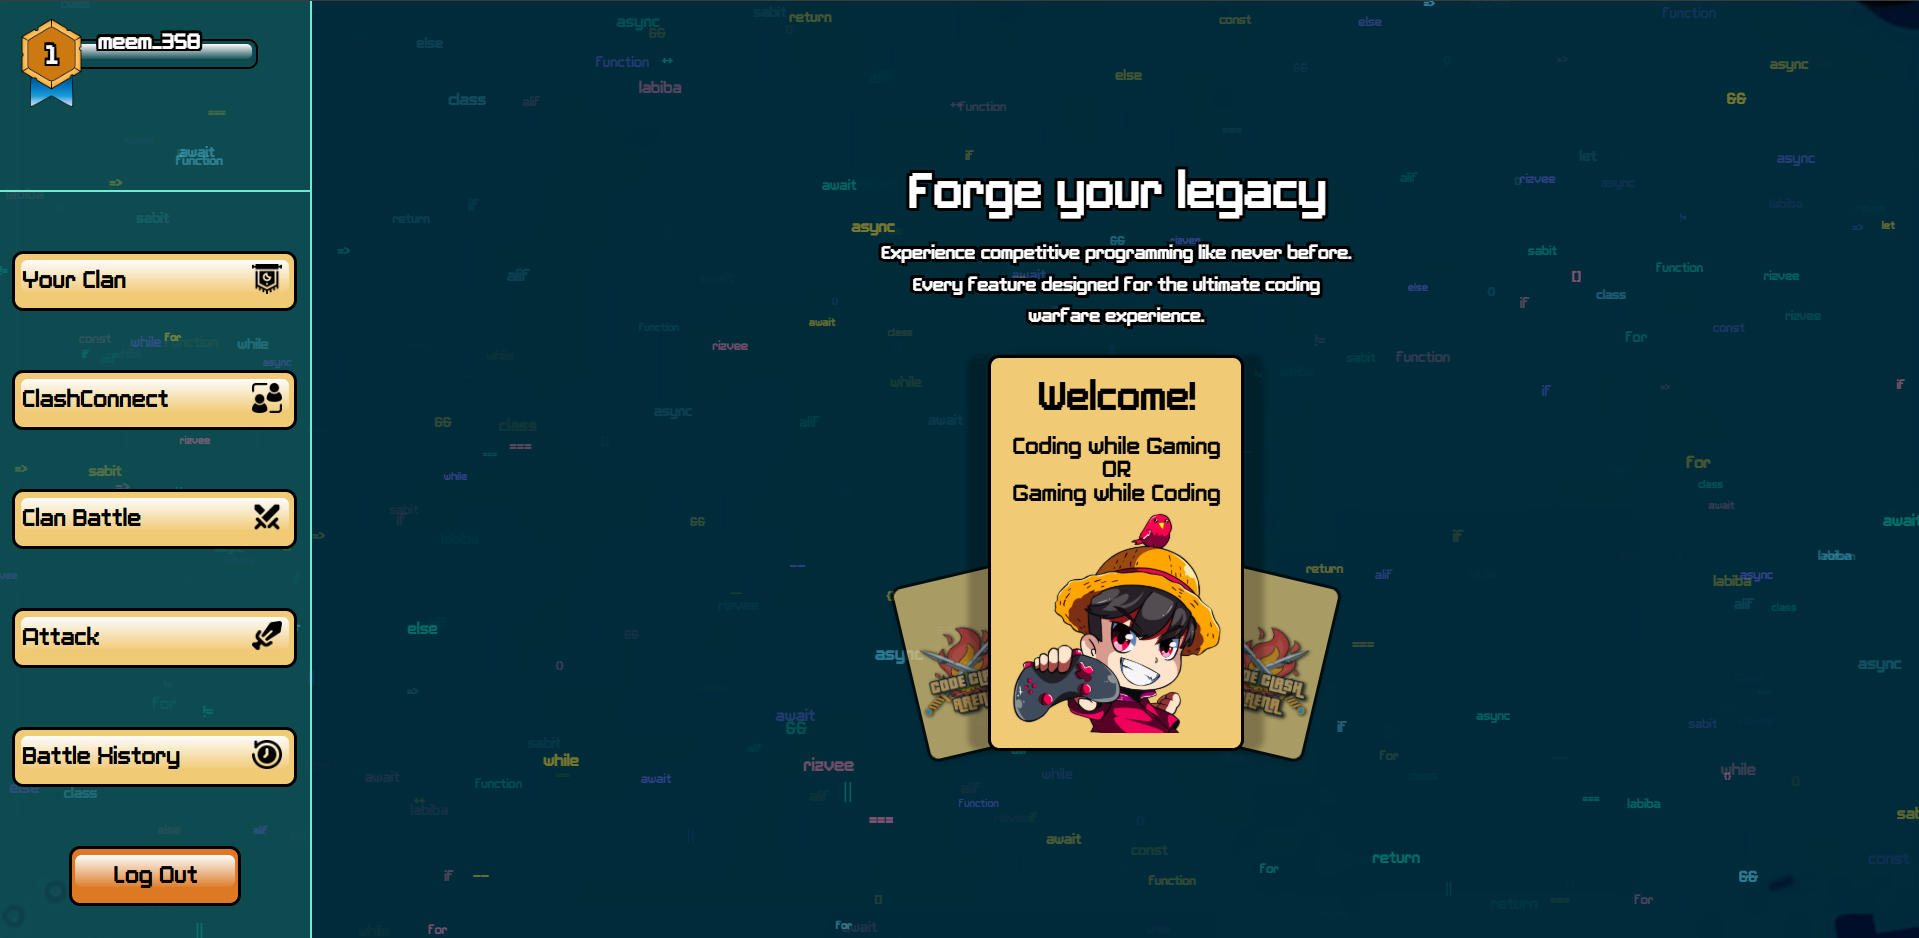
\includegraphics[width=0.95\textwidth]{maindasboard.png}
\caption{Main Dashboard - After successful login}
\label{fig:dashboard}
\end{figure}

\textbf{Common Login Errors and Solutions:}

\begin{longtable}{|p{5cm}|p{8.5cm}|}
\hline
\textbf{Error Message} & \textbf{Solution} \\
\hline
\endhead

"Invalid email or password" or authentication error & Verify email and password are correct; check for typos; ensure Caps Lock is off; verify email has been verified via link sent during signup \\
\hline

"Email not verified" & Check your email inbox for verification link; you must verify email before logging in; check spam/junk folder \\
\hline

"Account not found" & Email may not be registered; try signing up or verify correct email address \\
\hline

"Too many login attempts" & Wait 15 minutes before trying again; security measure against brute force attacks \\
\hline

"Network error" & Check internet connection; ensure stable connectivity; try refreshing page \\
\hline

\end{longtable}

\subsubsection{First-Time Login - Account Setup Complete}

After your first successful login:

\textbf{Codeforces Account Already Linked:}
\begin{itemize}[leftmargin=*]
\item Your Codeforces handle was linked during the sign-up process
\item No additional Codeforces setup is required
\item The system automatically retrieves your cf\_handle from the database upon login
\item This handle is used for all code submissions to Codeforces during battles
\item You can proceed immediately to explore the platform features
\end{itemize}

\textbf{If You Need to Update Codeforces Handle:}
\begin{enumerate}
\item Navigate to \textbf{Profile Settings} or \textbf{User Profile} section
\item Locate the \textbf{"Codeforces Handle"} field
\item Update your Codeforces username/handle if needed
\item Save changes
\item Note: Handle changes may be rate-limited to prevent abuse
\end{enumerate}


\textbf{Important}: Without a linked Codeforces account, you cannot participate in competitive battles or submit code solutions.

\FloatBarrier

\subsection{Logout Process}

Users can securely log out of their accounts at any time to end their session.

\subsubsection{Logout Steps}

\textbf{Step 1: Access User Menu}

\begin{itemize}[leftmargin=*]
\item Locate your username or profile icon in the top-right corner of the navigation bar
\item Click on the username/profile icon to open the dropdown menu
\item User menu will display with various options
\end{itemize}

\begin{figure}[!htb]
\centering
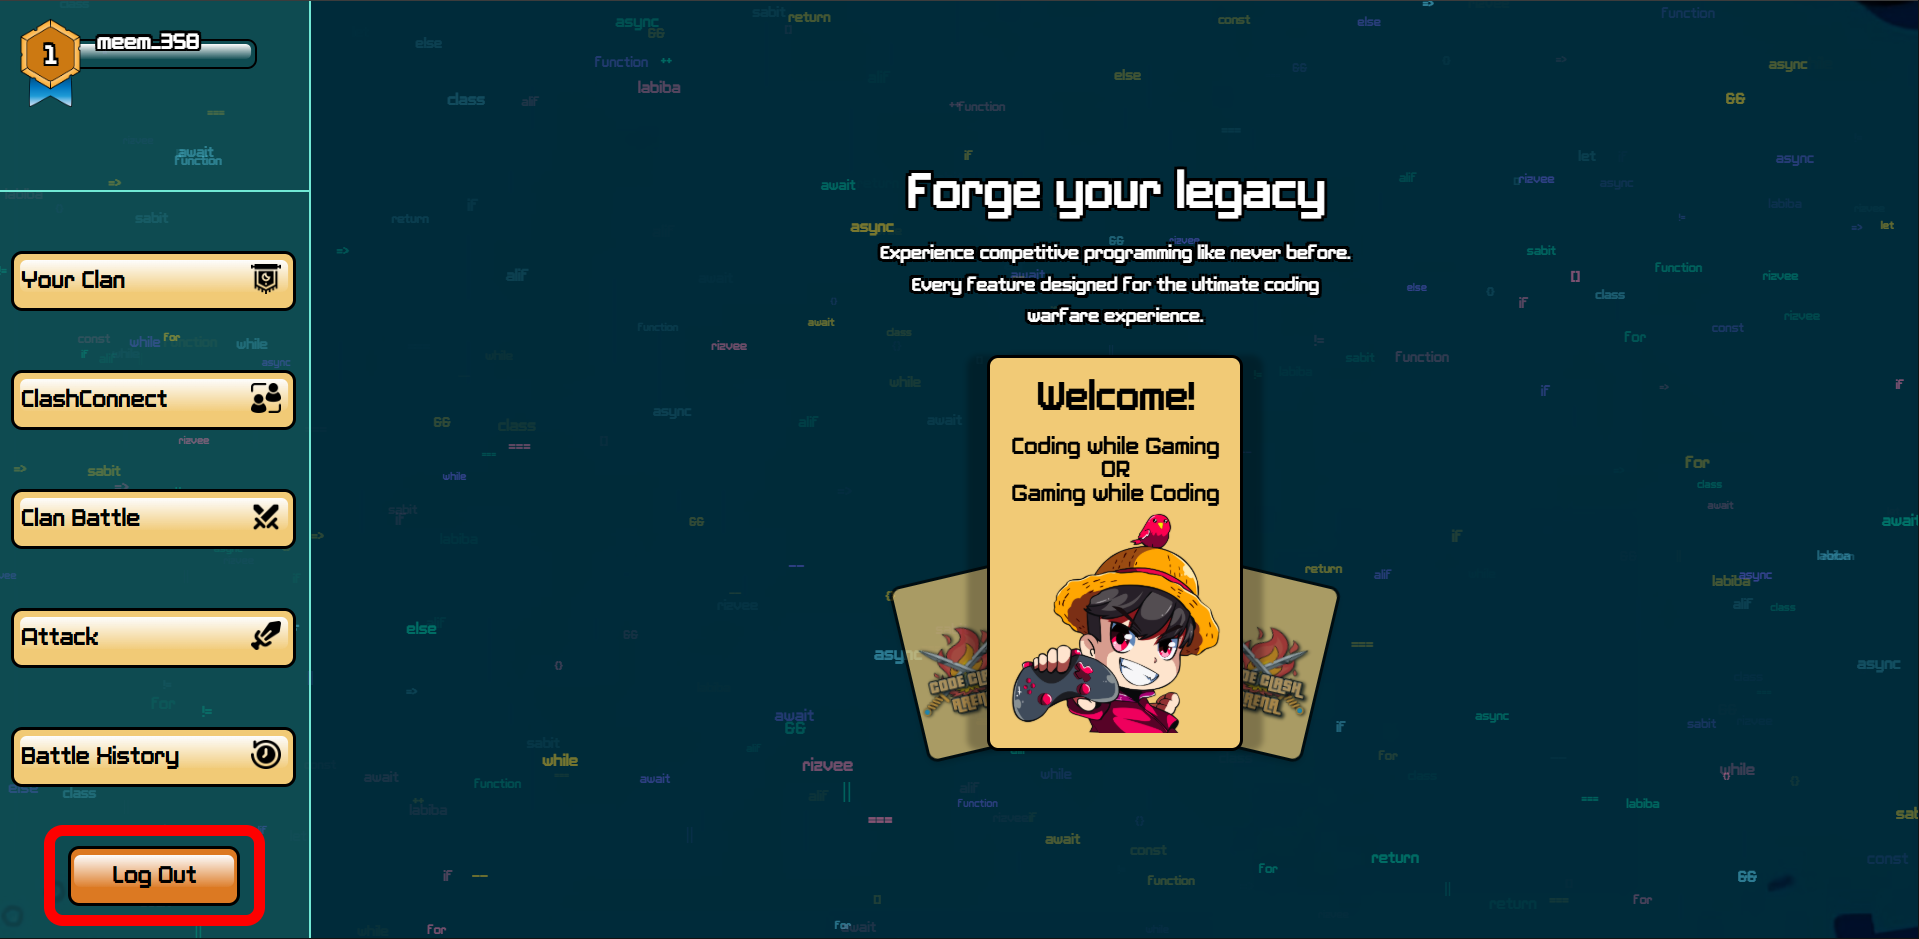
\includegraphics[width=0.9\textwidth]{logout.png}
\caption{User Menu - Access logout option}
\label{fig:user_menu}
\end{figure}

\textbf{Step 2: Select Logout Option}

\begin{itemize}[leftmargin=*]
\item From the dropdown menu, locate and click \textbf{"Logout"} or \textbf{"Sign Out"}
\item Option is typically at the bottom of the menu
\item May be represented by a logout icon (exit door or arrow)
\end{itemize}

\textbf{Step 3: Confirm Logout (if applicable)}

\begin{itemize}[leftmargin=*]
\item Confirmation dialog may appear: "Are you sure you want to logout?"
\item Click \textbf{"Yes"} or \textbf{"Confirm"} to proceed
\item Click \textbf{"Cancel"} to remain logged in
\item Some implementations may log out immediately without confirmation
\end{itemize}

\textbf{Step 4: Logout Completion}

\begin{itemize}[leftmargin=*]
\item Session is terminated on the server
\item Authentication tokens are cleared from browser
\item You are redirected to the homepage or login page
\item Confirmation message appears: "Successfully logged out"
\item All session data is cleared for security
\end{itemize}



\textbf{Important Security Notes:}
\begin{itemize}[leftmargin=*]
\item \textbf{Always logout on shared computers}: Prevent unauthorized access to your account
\item \textbf{Battle interruption}: If logged out during an active battle, it counts as forfeit
\item \textbf{Unsaved changes}: Any unsaved draft code in editor may be lost
\item \textbf{Session persistence}: "Remember Me" option keeps you logged in until explicit logout
\item \textbf{Automatic logout}: Sessions may expire after extended inactivity (typically 24-48 hours)
\end{itemize}

\FloatBarrier

\subsection{Troubleshooting Common Issues}

\subsubsection{Cannot Receive Verification/Reset Emails}

\textbf{Solutions:}
\begin{itemize}[leftmargin=*]
\item Check spam/junk folder for emails from Supabase
\item Verify email address was entered correctly during signup
\item Wait 5-10 minutes (email delivery may be delayed)
\item Whitelist emails from your authentication provider
\item Check email provider's filtering settings
\item Contact platform support if verification email is never received
\end{itemize}

\subsubsection{Account Locked After Multiple Failed Login Attempts}

\textbf{Solutions:}
\begin{itemize}[leftmargin=*]
\item Wait 15-30 minutes before attempting to login again
\item Ensure correct email and password are being used
\item Use password reset if password is forgotten
\item Contact support if issue persists after waiting period
\end{itemize}

\subsubsection{Browser Compatibility Issues}

\textbf{Solutions:}
\begin{itemize}[leftmargin=*]
\item Update browser to minimum required version (Chrome 84+, Firefox 103+, Safari 15+)
\item Enable JavaScript in browser settings
\item Clear browser cache and cookies
\item Disable browser extensions that may interfere
\item Try using a different supported browser
\end{itemize}

\subsection{Next Steps After Getting Started}

Once successfully logged in, proceed to:

\begin{enumerate}
\item \textbf{Explore Main Dashboard}: Familiarize yourself with navigation menu and available features - PvP Battles, Practice Gym, Clan Wars, and more
\item \textbf{Verify Codeforces Handle}: Your Codeforces handle was linked during signup - verify it appears correctly in your profile
\item \textbf{Complete Profile}: Add additional information, avatar, or bio (if available in profile settings)
\item \textbf{Browse Practice Gym}: Start with practice problems to familiarize yourself with the code editor and problem-solving interface
\item \textbf{Join or Create a Clan}: Team up with other coders for clan battles and collaborative competitions (optional)
\item \textbf{Enter First Battle}: Once comfortable, try a 1v1 PvP battle to experience competitive real-time coding
\end{enumerate}

\textbf{Recommended First Actions:}
\begin{itemize}[leftmargin=*]
\item Visit the \textbf{Practice Gym} to try solving a problem without time pressure
\item Check the \textbf{Leaderboard} to see top-ranked players
\item Read platform tutorials or help section (if available)
\item Configure notification preferences in settings
\end{itemize}

\FloatBarrier

% ==================================================
% SECTION 4: USER ROLES
% ==================================================

\section{User Roles}

CodeClash Arena is designed exclusively for authenticated registered users to ensure fair participation in competitive coding battles. Access to the platform requires account creation, email verification, and a linked Codeforces handle. There are no guest or admin roles in the system - all users have equal access to platform features and compete on a level playing field based on their coding skills and performance.

\subsection{Registered User}

A registered user is any individual who has successfully completed the sign-up process, verified their email address, and linked a valid Codeforces handle to their account. This is the only role on the platform, and all authenticated users operate with the same base permissions.

\subsubsection{Permissions}

Registered users have access to the following platform features:

\begin{itemize}[leftmargin=*]
\item \textbf{Account Management}: Register an account with email and Codeforces handle, log in and log out securely, update profile information and preferences
\item \textbf{Real-Time 1v1 Coding Battles}: Participate in Local battles (challenge specific friends with custom settings), participate in Global battles (matchmaking with players of similar skill level), compete in time-based coding challenges with live synchronization
\item \textbf{Clan System}: Create a new clan or join existing clans, participate in clan battles when selected by clan leader, contribute to clan rankings and statistics, manage clan memberships (leaders can approve/reject join requests)
\item \textbf{Code Submission}: Submit code solutions in multiple programming languages (C++, Java, Python, JavaScript, etc.), receive automated verdicts from Codeforces judge (Accepted, Wrong Answer, Time Limit Exceeded, etc.), test code locally using integrated code editor
\item \textbf{Statistics and Rankings}: View personal battle history and performance metrics, track XP, level, and ELO-based rating progression, access global and clan leaderboards, view detailed submission verdicts and problem-solving statistics
\item \textbf{Practice Mode}: Access Practice Gym with thousands of Codeforces problems, filter problems by difficulty, tags, and rating range, receive AI-based logical hints for approach guidance (without revealing full solutions), solve problems without time pressure for skill improvement
\item \textbf{Social Features}: Send and accept friend requests, view friend profiles and statistics, receive notifications for clan join requests and battle invitations
\end{itemize}

\subsubsection{Restrictions}

Registered users are subject to the following restrictions to maintain platform integrity and fair competition:

\begin{itemize}[leftmargin=*]
\item \textbf{No System Modifications}: Users cannot modify system configurations, settings, or platform code
\item \textbf{No Ranking Manipulation}: Direct manipulation of ratings, XP, leaderboards, or battle outcomes is strictly prohibited
\item \textbf{No Private Data Access}: Users cannot access other users' private information, submission code, or system database records
\item \textbf{No Unauthorized Authentication}: Users cannot share accounts or use multiple accounts to gain unfair advantages
\item \textbf{Fair Play Requirements}: Code submissions must be original work; plagiarism or copying solutions is not permitted
\end{itemize}

\FloatBarrier

% ==================================================
% SECTION 5: FEATURES AND FUNCTIONALITY
% ==================================================

\section{Features and Functionality}

This section provides detailed explanations of all major features available in CodeClash Arena, including step-by-step usage instructions, input/output descriptions, and visual guidance through UI screenshots.

% ==================================================
\subsection{PvP Battle System}

The Player vs Player (PvP) battle system is the core competitive feature of CodeClash Arena, allowing users to engage in real-time coding competitions. The system offers two distinct battle modes: Global Battle Mode for matchmaking with similarly skilled opponents, and Local Battle Mode for challenging specific friends with customizable settings.

\subsubsection{Global Battle Mode}

\textbf{Purpose:} Global Battle Mode provides an automated matchmaking system that pairs you with opponents of similar skill level for fair and competitive 1v1 coding battles. Your rating changes based on battle outcomes and opponent strength using an ELO-based ranking system.

\textbf{Step-by-Step Usage:}

\textbf{Step 1: Access Global Battle Mode}
\begin{enumerate}
\item From the Main Dashboard, locate the \textbf{"Attack"} button on the left navigation menu
\item Click the \textbf{"Attack"} button to open the battle mode selection overlay
\item The overlay menu displays two modes: \textbf{1v1} and \textbf{Practice}
\item Click on \textbf{"1v1"} mode
\item A submenu appears with two options: \textbf{Global} and \textbf{Local}
\item Click on \textbf{"Global"} option (for matchmaking with similar-rated opponents)
\item The Global Battle interface loads
\end{enumerate}

\begin{figure}[!htb]
\centering
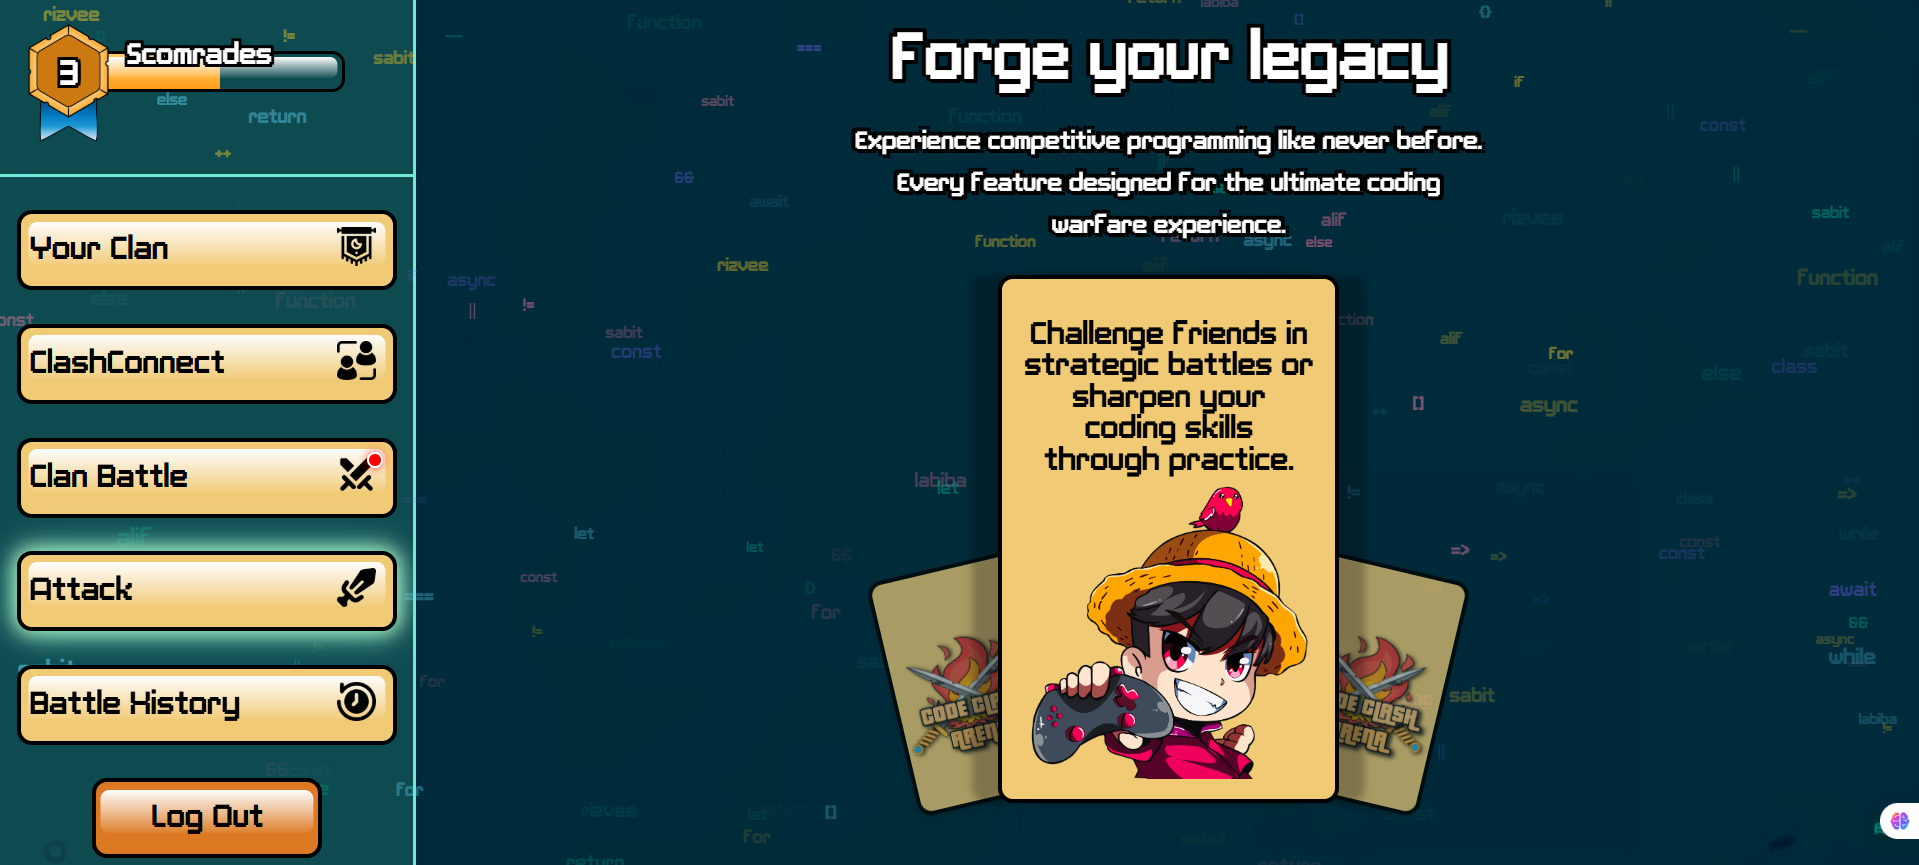
\includegraphics[width=0.9\textwidth]{Homepage_attack_highlighted.png}
\caption{Main Dashboard - Click Attack button to access battle modes}
\label{fig:attack_button}
\end{figure}

\textbf{Step 2: Enter Matchmaking Queue}
\begin{enumerate}
\item On the Global Battle page, you will see your current rating, level, and matchmaking options
\item Click the \textbf{"Find Match"} or \textbf{"Start Matchmaking"} button
\item The system searches for an available opponent with similar rating (±200 rating range)
\item A loading/searching animation displays with message: "Searching for opponent..."
\item Queue time varies based on available players (typically 10-60 seconds)
\item You can cancel matchmaking by clicking \textbf{"Cancel Search"} button
\end{enumerate}

\begin{figure}[!htb]
\centering
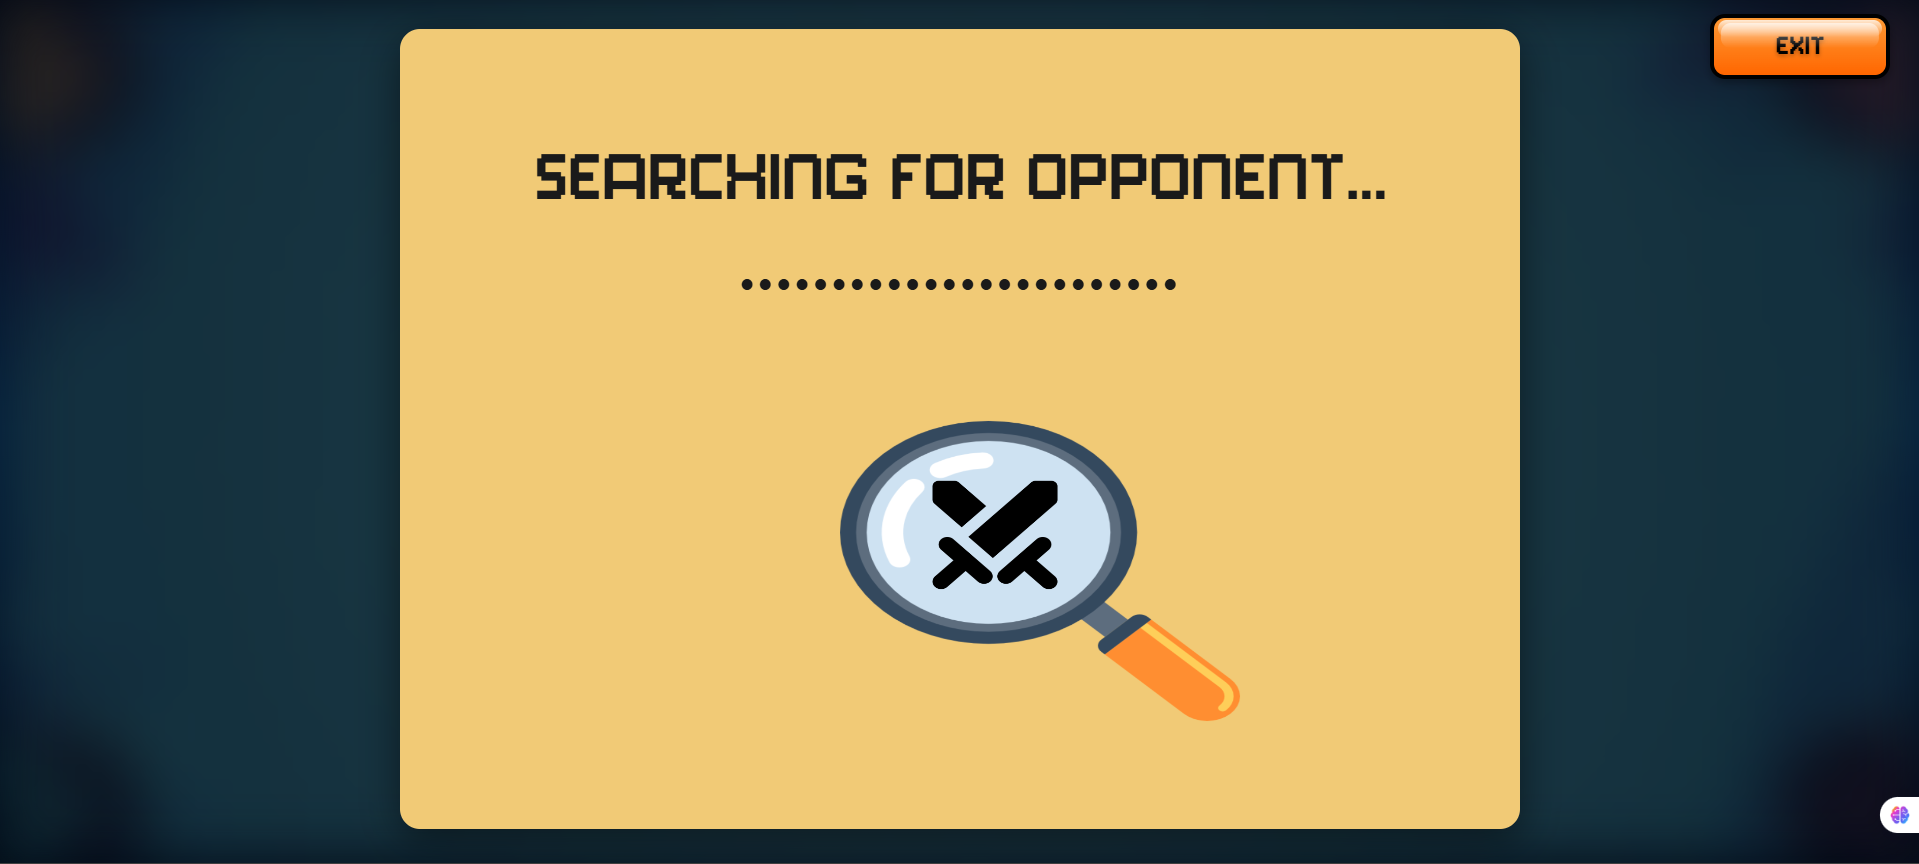
\includegraphics[width=0.9\textwidth]{global_mode_searching.png}
\caption{Global Battle - Enter matchmaking queue}
\label{fig:global_matchmaking}
\end{figure}

\textbf{Step 3: Match Found - Battle Initialization}
\begin{enumerate}
\item When an opponent is found, a notification appears: "Opponent Found!"
\item Opponent's username, rating, and level are displayed
\item Battle settings are shown:
  \begin{itemize}
    \item Problem difficulty (automatically selected based on average rating)
    \item Battle duration (standard time limit, typically 30-45 minutes)
    \item Programming languages allowed
  \end{itemize}
\item Countdown timer begins (3-5 seconds) before battle starts
\item Both players are synchronized and enter the battle arena simultaneously
\end{enumerate}

\begin{figure}[!htb]
\centering
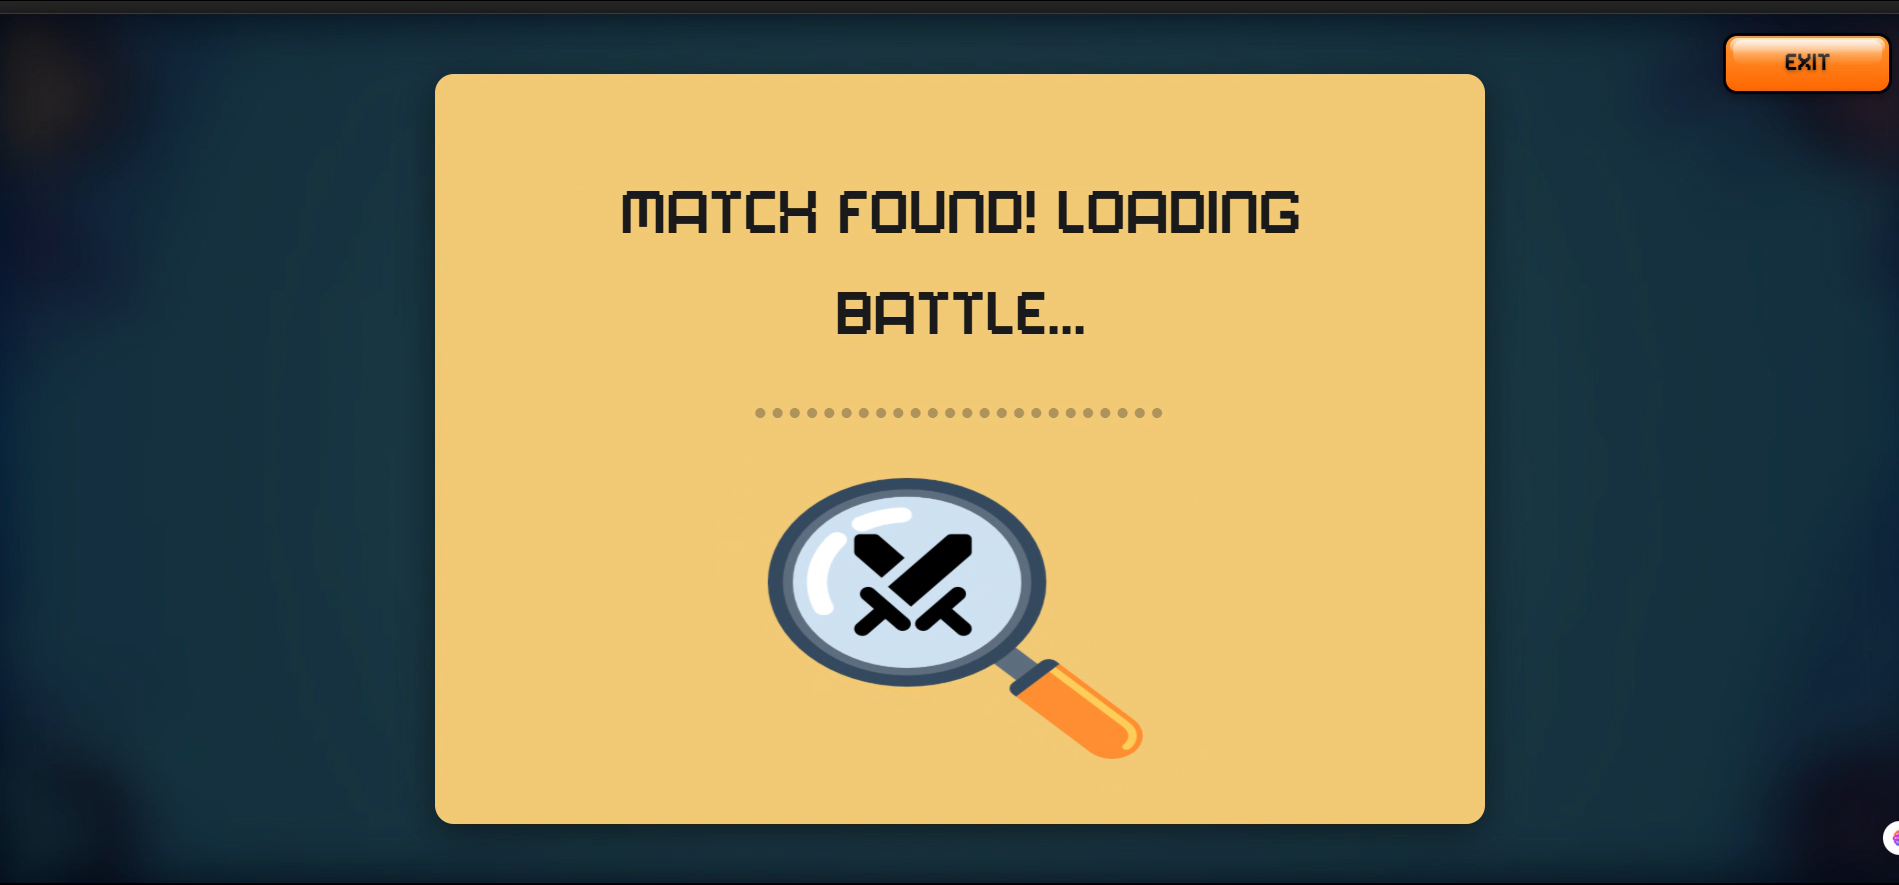
\includegraphics[width=0.9\textwidth]{global_match_found.png}
\caption{Match Found - Opponent details and battle initialization}
\label{fig:match_found}
\end{figure}

\textbf{Step 4: Battle Arena Interface}
\begin{enumerate}
\item Battle arena loads with split-screen layout:
  \begin{itemize}
    \item \textbf{Left Panel}: Problem statement (Codeforces problem embedded in iframe)
    \item \textbf{Right Panel}: Code editor with syntax highlighting
    \item \textbf{Top Bar}: Battle timer, your username, opponent username, submission status indicators
  \end{itemize}
\item Battle timer starts counting down from the allocated time
\item Read the problem statement carefully
\item Opponent's submission status is visible in real-time (e.g., "Opponent is coding...", "Opponent submitted")
\end{enumerate}

\begin{figure}[!htb]
\centering
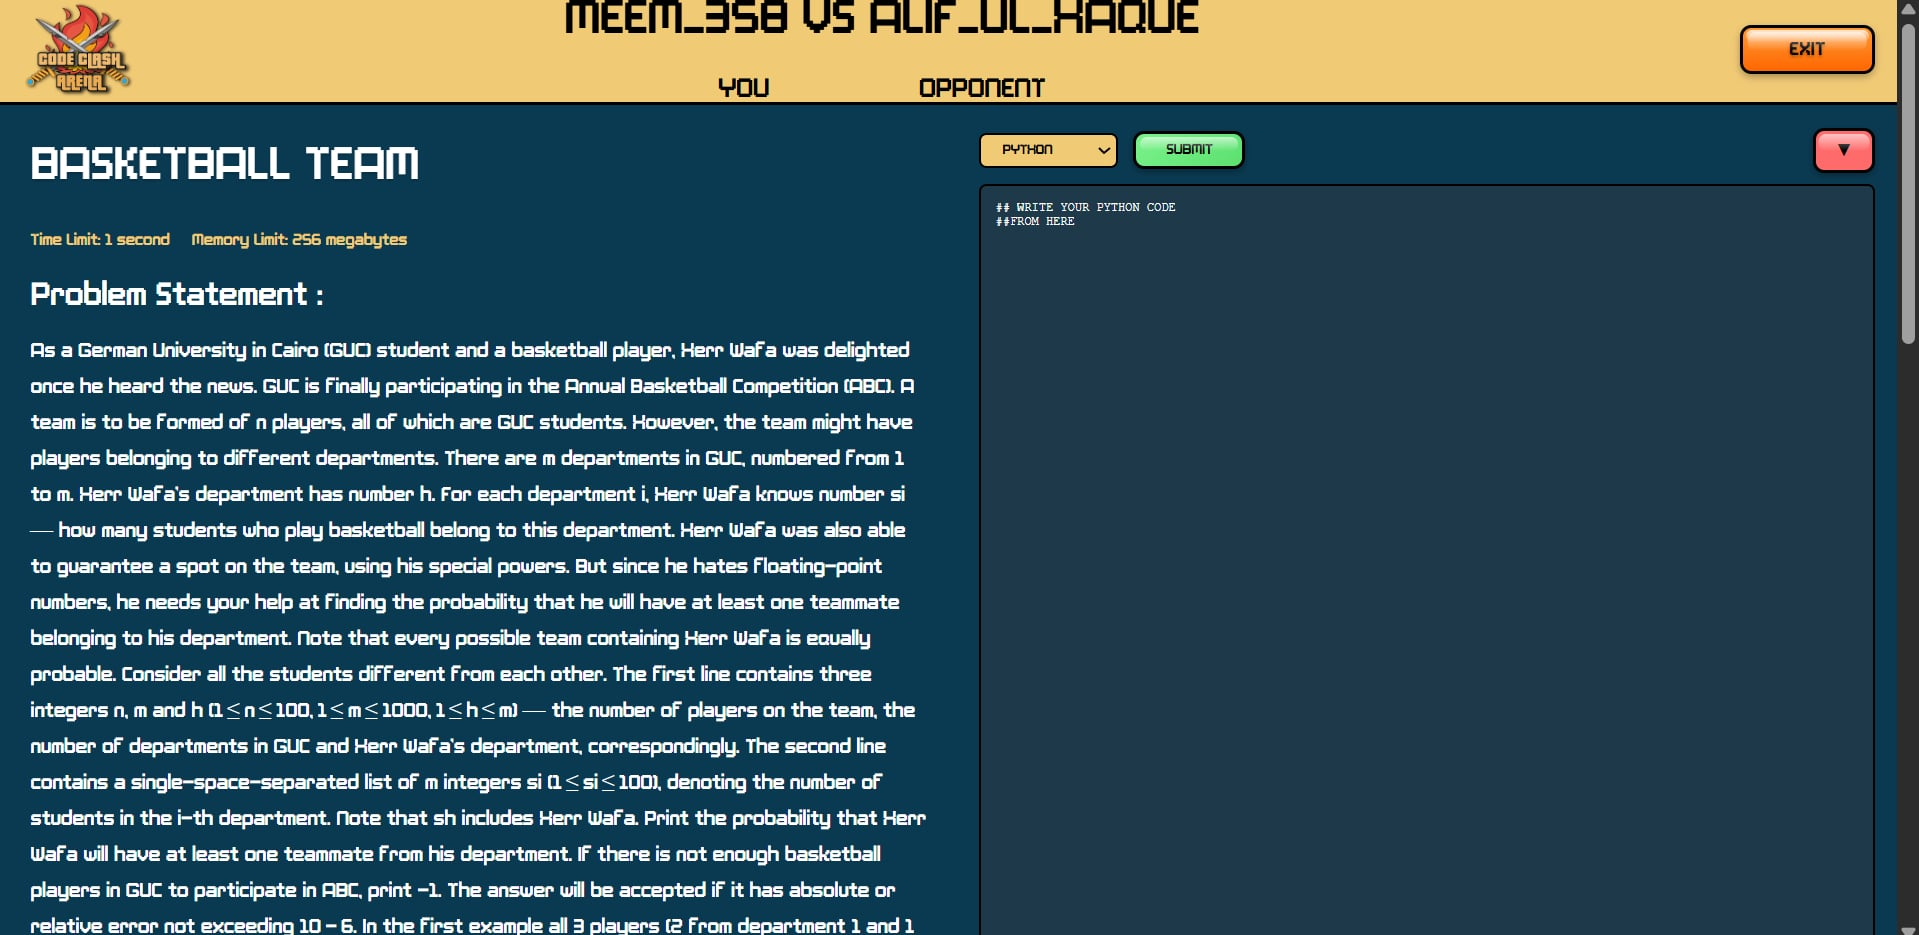
\includegraphics[width=0.9\textwidth]{battle_arena.png}
\caption{Battle Arena - Split-screen interface with problem and editor}
\label{fig:battle_arena}
\end{figure}

\textbf{Step 5: Writing and Testing Code}
\begin{enumerate}
\item Select your preferred programming language from the language dropdown menu (C++, Java, Python, JavaScript, etc.)
\item Write your solution code in the integrated editor
\item Use the \textbf{"Run Code"} or \textbf{"Test"} button to test your code locally:
  \begin{itemize}
    \item Input sample test cases manually
    \item View output and execution time
    \item Debugging assistance through local testing (uses Piston API)
  \end{itemize}
\item Fix any errors or logic issues identified during testing
\item Refine your solution for edge cases
\end{enumerate}

\textbf{Step 6: Submitting Solution}
\begin{enumerate}
\item Once confident in your solution, click the \textbf{"Submit"} button
\item Code is sent to Codeforces judge for official evaluation
\item Submission status appears: "Submitting..." → "In Queue" → "Running on Test X"
\item Wait for verdict (typically 5-15 seconds, depending on Codeforces server load)
\item Verdict is displayed:
  \begin{itemize}
    \item \textbf{Accepted (AC)}: All test cases passed - you win the battle!
    \item \textbf{Wrong Answer (WA)}: Failed test case - you can resubmit
    \item \textbf{Time Limit Exceeded (TLE)}: Code too slow - optimize and resubmit
    \item \textbf{Runtime Error (RE)}: Code crashed - fix bugs and resubmit
    \item \textbf{Compilation Error (CE)}: Syntax errors - fix and resubmit
  \end{itemize}
\item You can submit multiple times until you get Accepted or time runs out
\end{enumerate}

\begin{figure}[!htb]
\centering
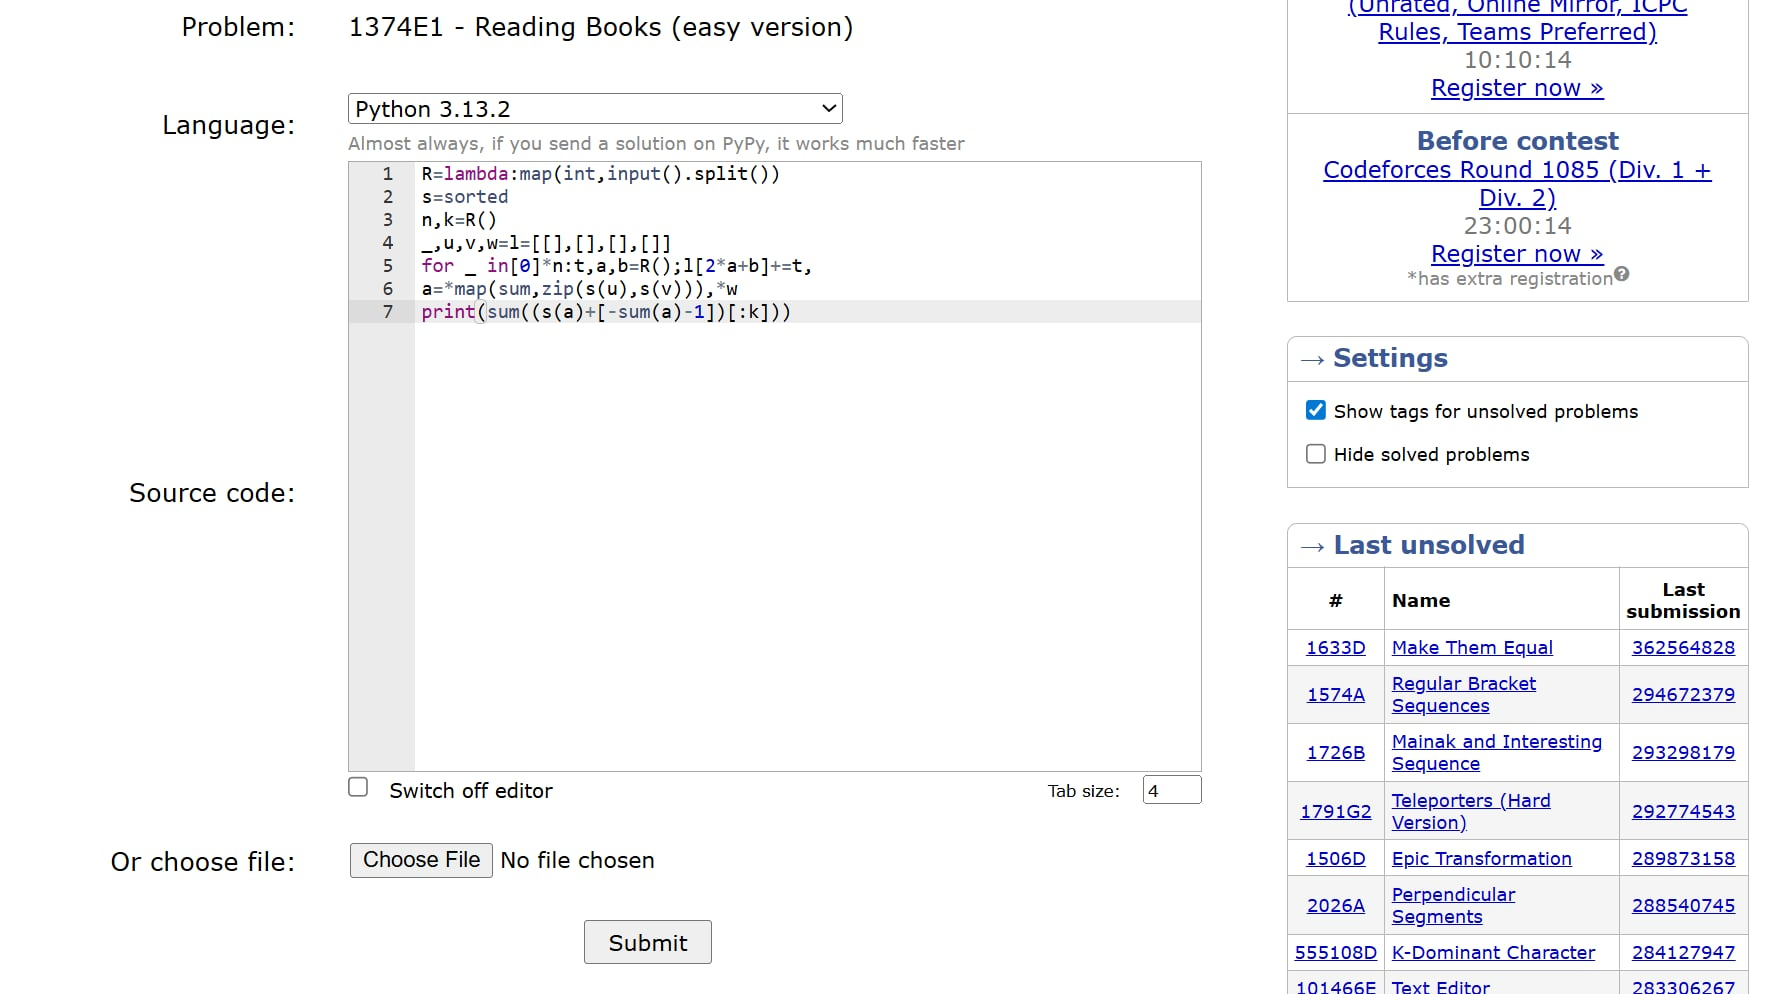
\includegraphics[width=0.9\textwidth]{cf_interface.png}
\caption{Code Submission - Submit button and verdict display}
\label{fig:code_submit}
\end{figure}

\textbf{Step 7: Battle Conclusion}
\begin{enumerate}
\item Battle ends when:
  \begin{itemize}
    \item One player gets Accepted verdict (winner determined)
    \item Battle timer reaches zero (player with most progress wins, or draw if equal)
    \item Both players get Accepted (first to submit wins)
  \end{itemize}
\item Battle result screen displays:
  \begin{itemize}
    \item Winner/Loser announcement
    \item Final submission status for both players
    \item Time taken by each player
    \item Rating change (e.g., "+15 rating" for winner, "-12 rating" for loser)
    \item XP earned (winners earn more XP)
  \end{itemize}
\item Battle summary is added to Battle History
\item Click \textbf{"Return to Dashboard"} to exit battle arena
\end{enumerate}

\begin{figure}[!htb]
\centering
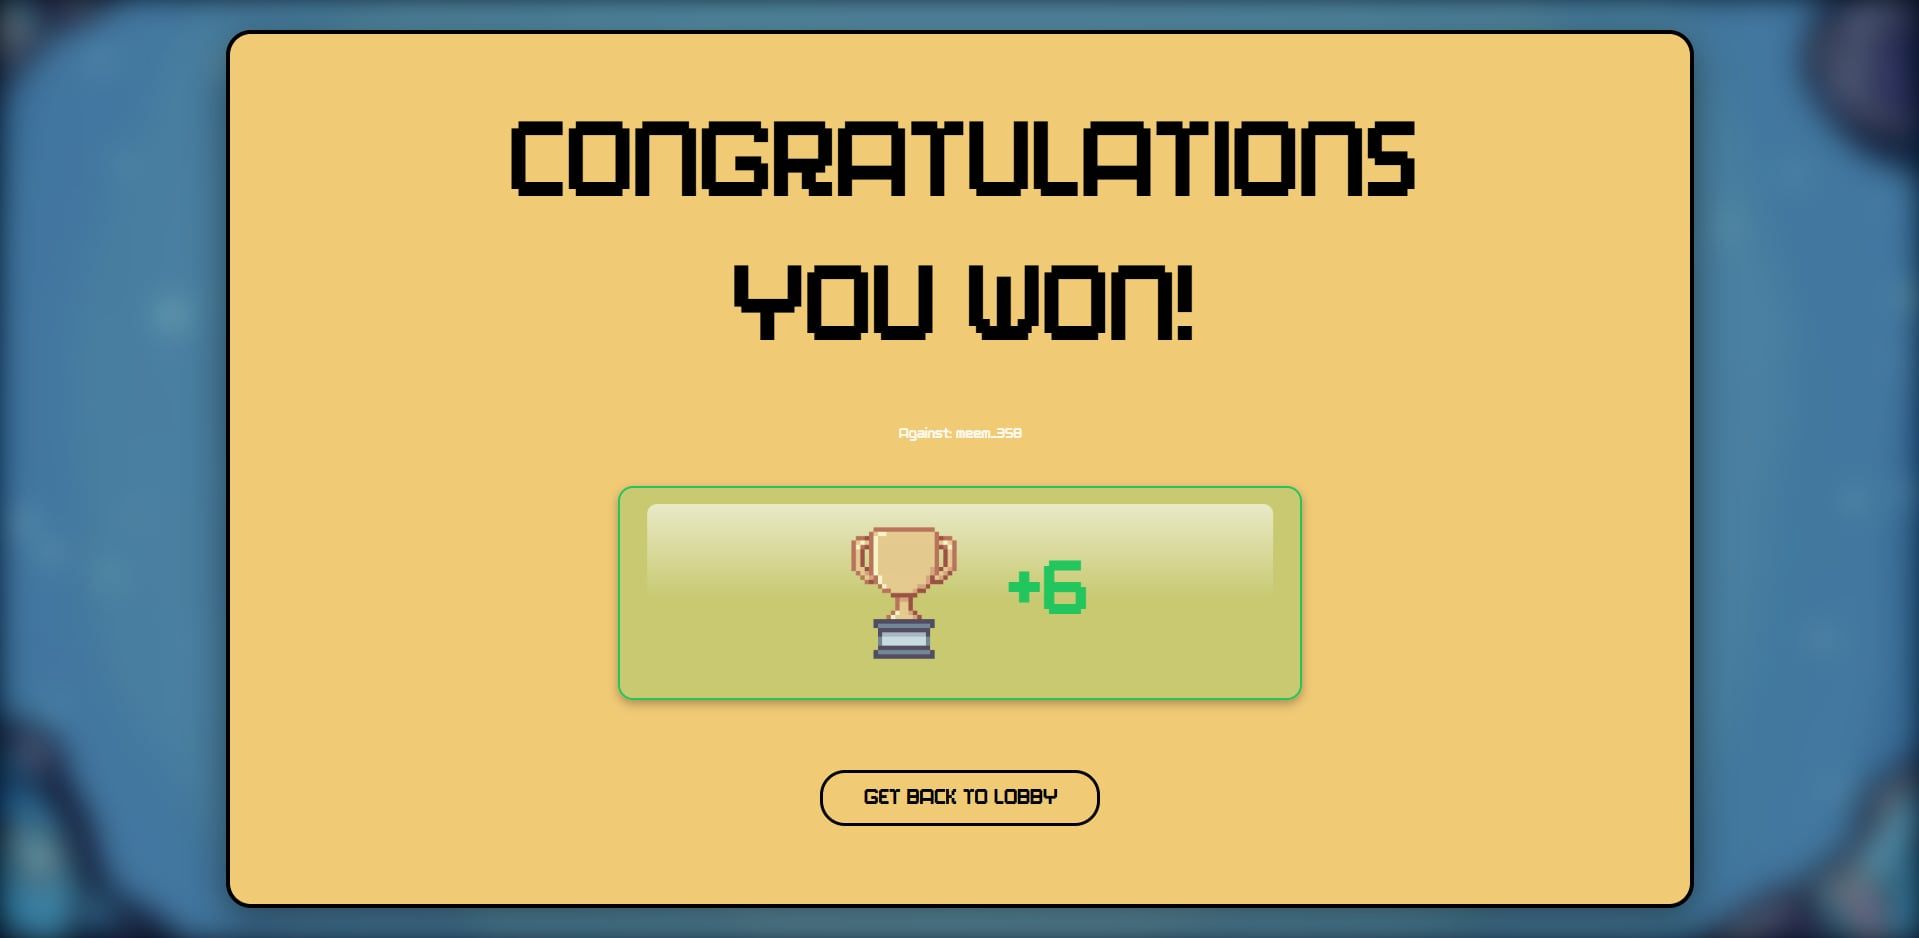
\includegraphics[width=0.9\textwidth]{local_battle_ended.png}
\caption{Battle Result - Winner announcement and statistics}
\label{fig:battle_result}
\end{figure}

\textbf{Input Requirements:}
\begin{itemize}[leftmargin=*]
\item \textbf{Player Prerequisites}: Valid CodeClash Arena account, linked Codeforces handle, stable internet connection (5+ Mbps)
\item \textbf{Matchmaking Input}: Player rating (automatically used for matchmaking), availability in matchmaking pool
\item \textbf{Code Input}: Solution code in selected programming language, must compile without syntax errors
\end{itemize}

\textbf{Output and Results:}
\begin{itemize}[leftmargin=*]
\item \textbf{Matchmaking Output}: Opponent found with username, rating, level
\item \textbf{Battle Output}: Real-time battle interface with synchronized timer, problem statement, code editor
\item \textbf{Submission Output}: Official Codeforces verdict (AC, WA, TLE, RE, CE, etc.), test case results, execution time
\item \textbf{Battle Conclusion Output}: Win/Loss/Draw result, rating change (ELO-based calculation), XP earned, updated statistics in profile, battle record in history
\end{itemize}

\textbf{Special Features:}
\begin{itemize}[leftmargin=*]
\item \textbf{Real-Time Synchronization}: See opponent's submission status live ("Opponent submitted", "Opponent got Accepted")
\item \textbf{Automatic Forfeiture}: Disconnection for >30 seconds results in automatic loss
\item \textbf{Fair Matchmaking}: Rating-based pairing ensures competitive balance
\item \textbf{Multiple Submissions}: Unlimited submission attempts during battle time
\end{itemize}

\FloatBarrier

\subsubsection{Local Battle Mode}

\textbf{Purpose:} Local Battle Mode allows you to challenge specific friends or users directly, with customizable battle settings including problem difficulty, time limits, and problem selection. This mode is ideal for practice with friends or organizing custom competitions.

\textbf{Step-by-Step Usage:}

\textbf{Step 1: Access Local Battle Mode}
\begin{enumerate}
\item From the Main Dashboard, click the \textbf{"Attack"} button on the left navigation menu
\item The battle mode selection overlay displays two modes: \textbf{1v1} and \textbf{Practice}
\item Click on \textbf{"1v1"} mode
\item A submenu appears with two options: \textbf{Global} and \textbf{Local}
\item Click on \textbf{"Local"} option (for challenging specific friends)
\item The Local Battle configuration page loads
\end{enumerate}

\begin{figure}[!htb]
\centering
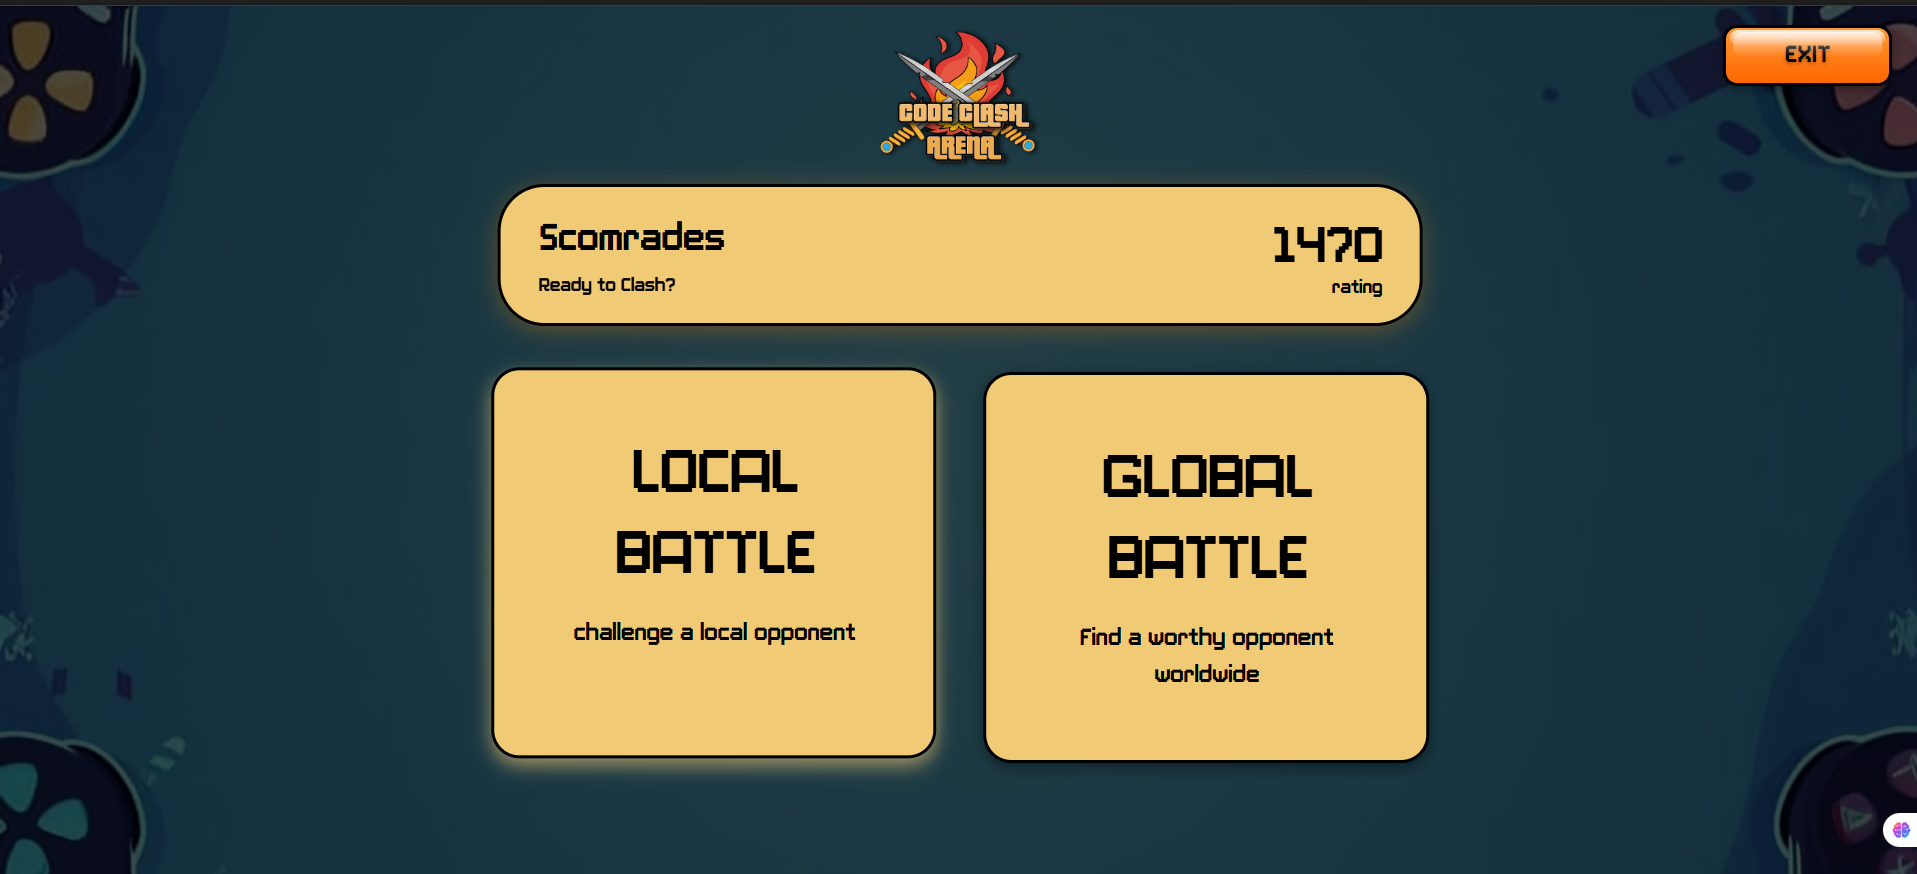
\includegraphics[width=0.9\textwidth]{select_local_battle.png}
\caption{Battle Mode Selection - Local Battle option}
\label{fig:local_battle_select}
\end{figure}

\textbf{Step 2: Configure Battle Settings}
\begin{enumerate}
\item On the Local Battle setup page, configure the following settings:
  \begin{itemize}
    \item \textbf{Opponent Selection}:
      \begin{itemize}
        \item Enter opponent's username/handle in the search field
        \item System validates that user exists
        \item Friend list may be displayed for quick selection
      \end{itemize}
    \item \textbf{Problem Difficulty}:
      \begin{itemize}
        \item Select from difficulty levels: Easy (800-1200 rating), Medium (1200-1800 rating), Hard (1800-2400 rating), Expert (2400+)
        \item Or specify exact Codeforces rating range
      \end{itemize}
    \item \textbf{Time Limit}:
      \begin{itemize}
        \item Choose battle duration: 15 minutes, 30 minutes, 45 minutes, 60 minutes, or custom
      \end{itemize}
    \item \textbf{Problem Selection} (Optional):
      \begin{itemize}
        \item Let system auto-select from difficulty range
        \item Or manually specify a Codeforces problem by contest ID and problem letter
      \end{itemize}
  \end{itemize}
\item Review all settings before proceeding
\end{enumerate}

\begin{figure}[!htb]
\centering
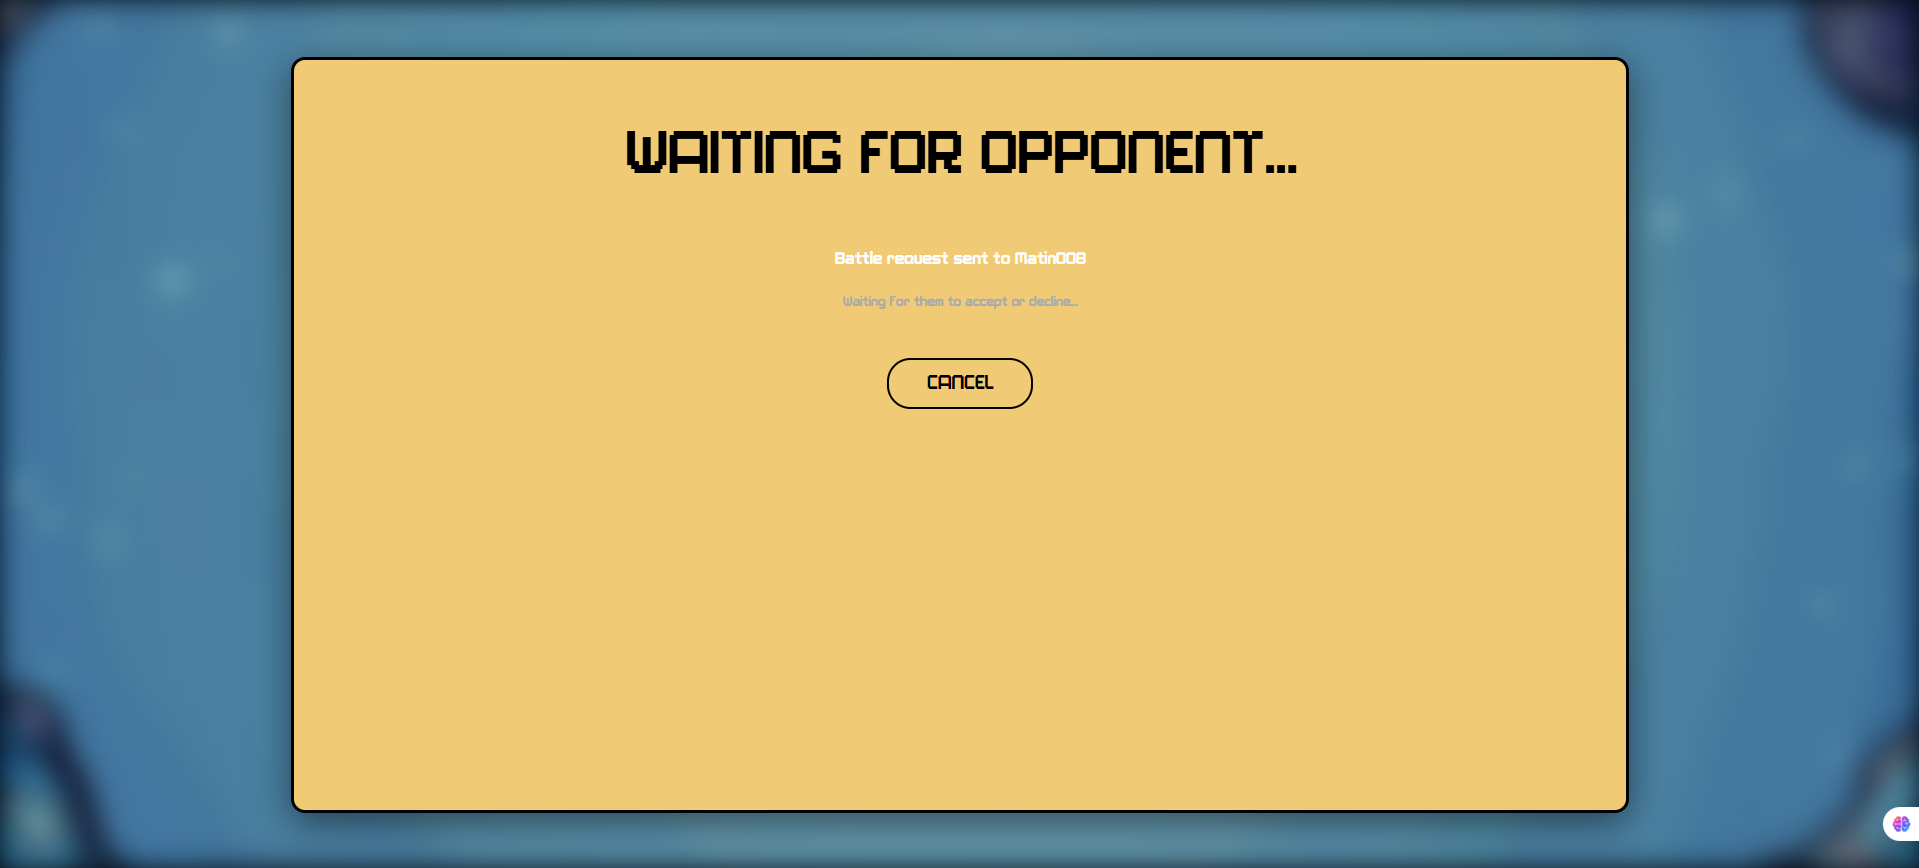
\includegraphics[width=0.9\textwidth]{send_battle_request.png}
\caption{Local Battle Configuration - Battle settings customization}
\label{fig:local_battle_config}
\end{figure}

\textbf{Step 3: Send Battle Invitation}
\begin{enumerate}
\item After configuring settings, click the \textbf{"Send Challenge"} or \textbf{"Invite to Battle"} button
\item System validates that opponent is online and available
\item Battle invitation is sent to the opponent with configured settings displayed
\item You see a waiting screen: "Waiting for [opponent name] to accept..."
\item Invitation includes:
  \begin{itemize}
    \item Your username as challenger
    \item Selected difficulty and time limit
    \item Option to accept or decline
  \end{itemize}
\item You can cancel the invitation while waiting by clicking \textbf{"Cancel Invitation"}
\end{enumerate}

\begin{figure}[!htb]
\centering
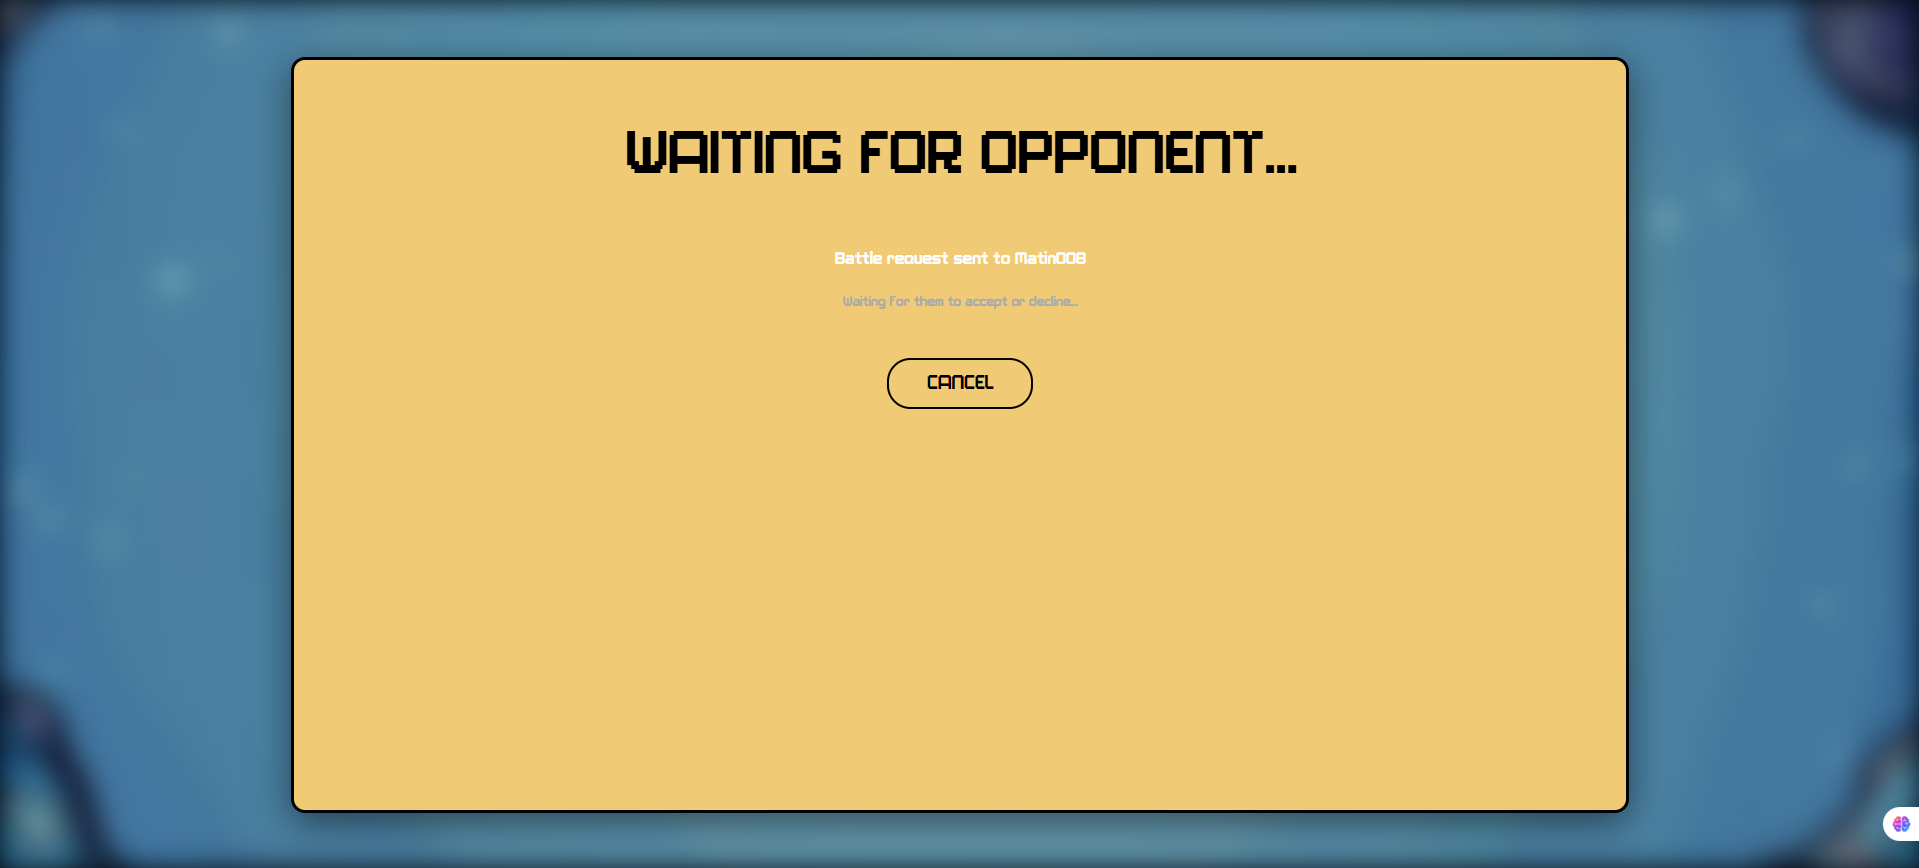
\includegraphics[width=0.9\textwidth]{send_battle_request.png}
\caption{Battle Invitation - Waiting for opponent acceptance}
\label{fig:battle_invitation_sent}
\end{figure}

\textbf{Step 4: Opponent Accepts - Battle Begins}
\begin{enumerate}
\item When opponent accepts, both players receive notification: "Battle Starting!"
\item Countdown timer (3-5 seconds) synchronizes both players
\item Battle arena loads with the configured problem and settings
\item Interface is identical to Global Battle mode:
  \begin{itemize}
    \item Problem statement on left
    \item Code editor on right
    \item Timer countdown from configured duration
    \item Opponent status visible in real-time
  \end{itemize}
\item Both players start coding simultaneously
\end{enumerate}

\begin{figure}[!htb]
\centering
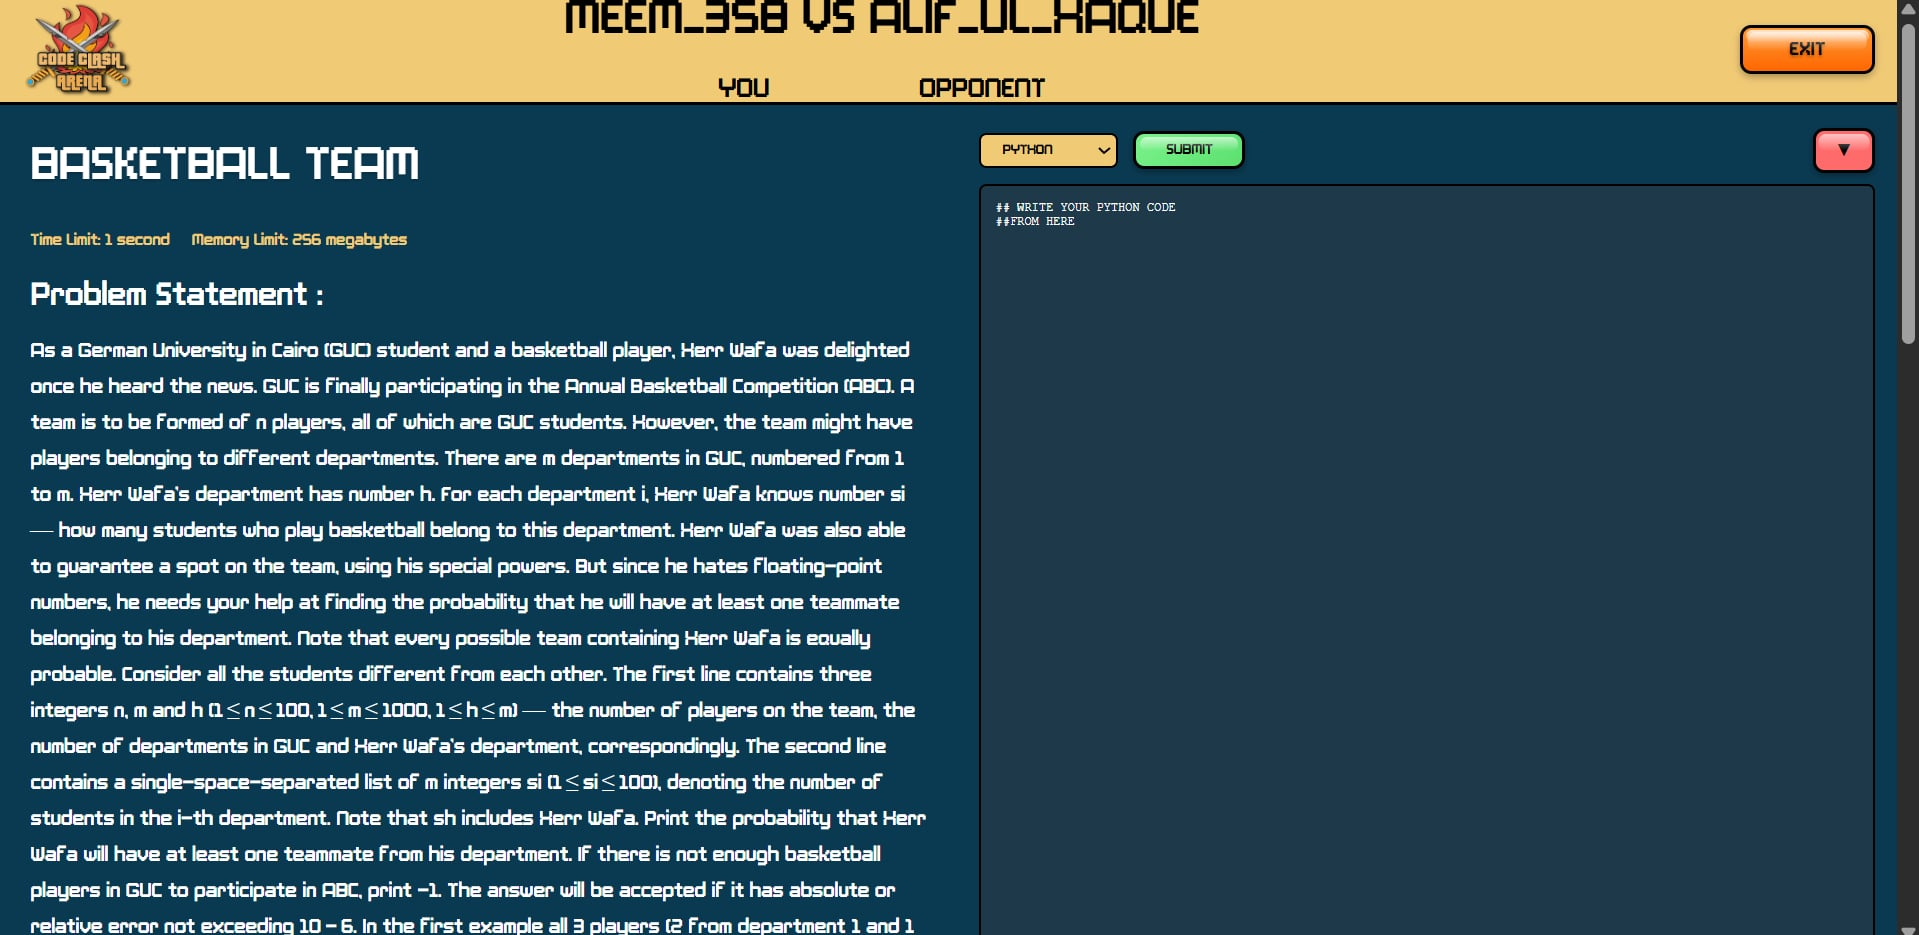
\includegraphics[width=0.9\textwidth]{battle_arena.png}
\caption{Local Battle Arena - Customized battle in progress}
\label{fig:local_battle_arena}
\end{figure}

\textbf{Step 5-7: Battle Execution}

The remaining steps (writing code, testing, submitting, and battle conclusion) follow the same process as Global Battle Mode (refer to Global Battle Mode Steps 5-7).

Key differences in Local Battle:
\begin{itemize}[leftmargin=*]
\item Battle uses your custom time limit (not standard duration)
\item Problem difficulty is as configured (not auto-selected by system)
\item Rating changes may be smaller or disabled (depending on implementation)
\item Results still recorded in Battle History
\end{itemize}

\textbf{Accepting Incoming Local Battle Invitations:}

When you receive a Local Battle invitation from another player:
\begin{enumerate}
\item Notification appears (popup or notification badge)
\item Click notification to view invitation details
\item Invitation shows: Challenger's name, difficulty level, time limit, problem (if specified)
\item Click \textbf{"Accept"} to enter battle, or \textbf{"Decline"} to reject
\item If accepted, battle arena loads immediately with countdown
\end{enumerate}

\begin{figure}[!htb]
\centering
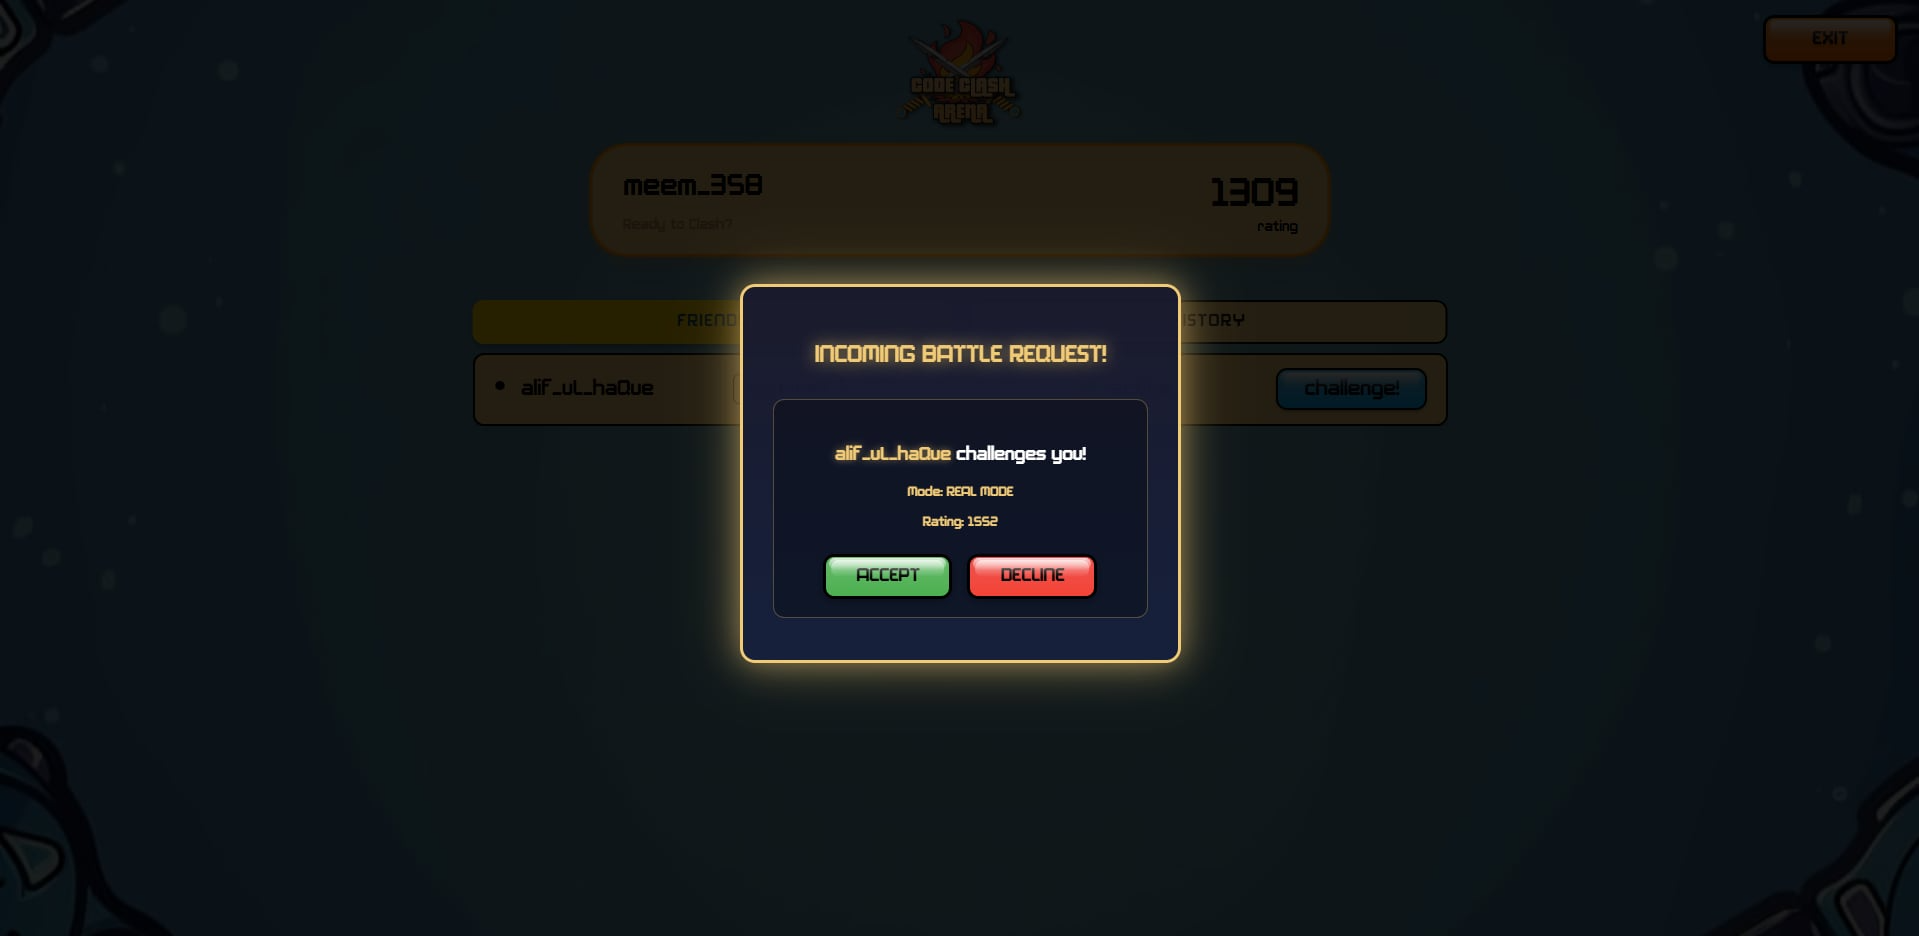
\includegraphics[width=0.9\textwidth]{incoming_battle_request.png}
\caption{Incoming Battle Invitation - Accept or Decline}
\label{fig:battle_invitation_received}
\end{figure}

\textbf{Input Requirements:}
\begin{itemize}[leftmargin=*]
\item \textbf{Challenger Input}: Opponent username (must exist and be online), difficulty selection, time limit, optional problem specification
\item \textbf{Opponent Input}: Accept or decline decision
\item \textbf{Code Input}: Solution code (same as Global Battle)
\end{itemize}

\textbf{Output and Results:}
\begin{itemize}[leftmargin=*]
\item \textbf{Invitation Output}: Invitation sent/received notification, waiting status
\item \textbf{Battle Output}: Custom battle arena with configured settings
\item \textbf{Results Output}: Battle outcome (Win/Loss/Draw), rating change (if applicable), XP earned, battle added to history
\end{itemize}

\textbf{Special Features:}
\begin{itemize}[leftmargin=*]
\item \textbf{Flexible Settings}: Complete control over difficulty and duration
\item \textbf{Friend Practice}: Practice with friends without rating pressure
\item \textbf{Custom Problems}: Specify exact problems for focused practice
\item \textbf{Invitation System}: Organized challenge workflow with accept/decline options
\end{itemize}

\FloatBarrier

% ==================================================
\subsection{Practice Gym}

\textbf{Purpose:} Practice Gym provides a solo training environment where you can solve coding problems without time pressure or competitive stress. Access thousands of Codeforces problems, filter by difficulty and tags, receive AI-based hints, and improve your skills at your own pace.

\textbf{Step-by-Step Usage:}

\textbf{Step 1: Access Practice Gym}
\begin{enumerate}
\item From the Main Dashboard, click the \textbf{"Attack"} button
\item The battle mode selection overlay displays two modes: \textbf{1v1} and \textbf{Practice}
\item Click on \textbf{"Practice"} option (for solo practice without time pressure)
\item Practice Gym interface loads showing problem browser
\end{enumerate}

\begin{figure}[!htb]
\centering
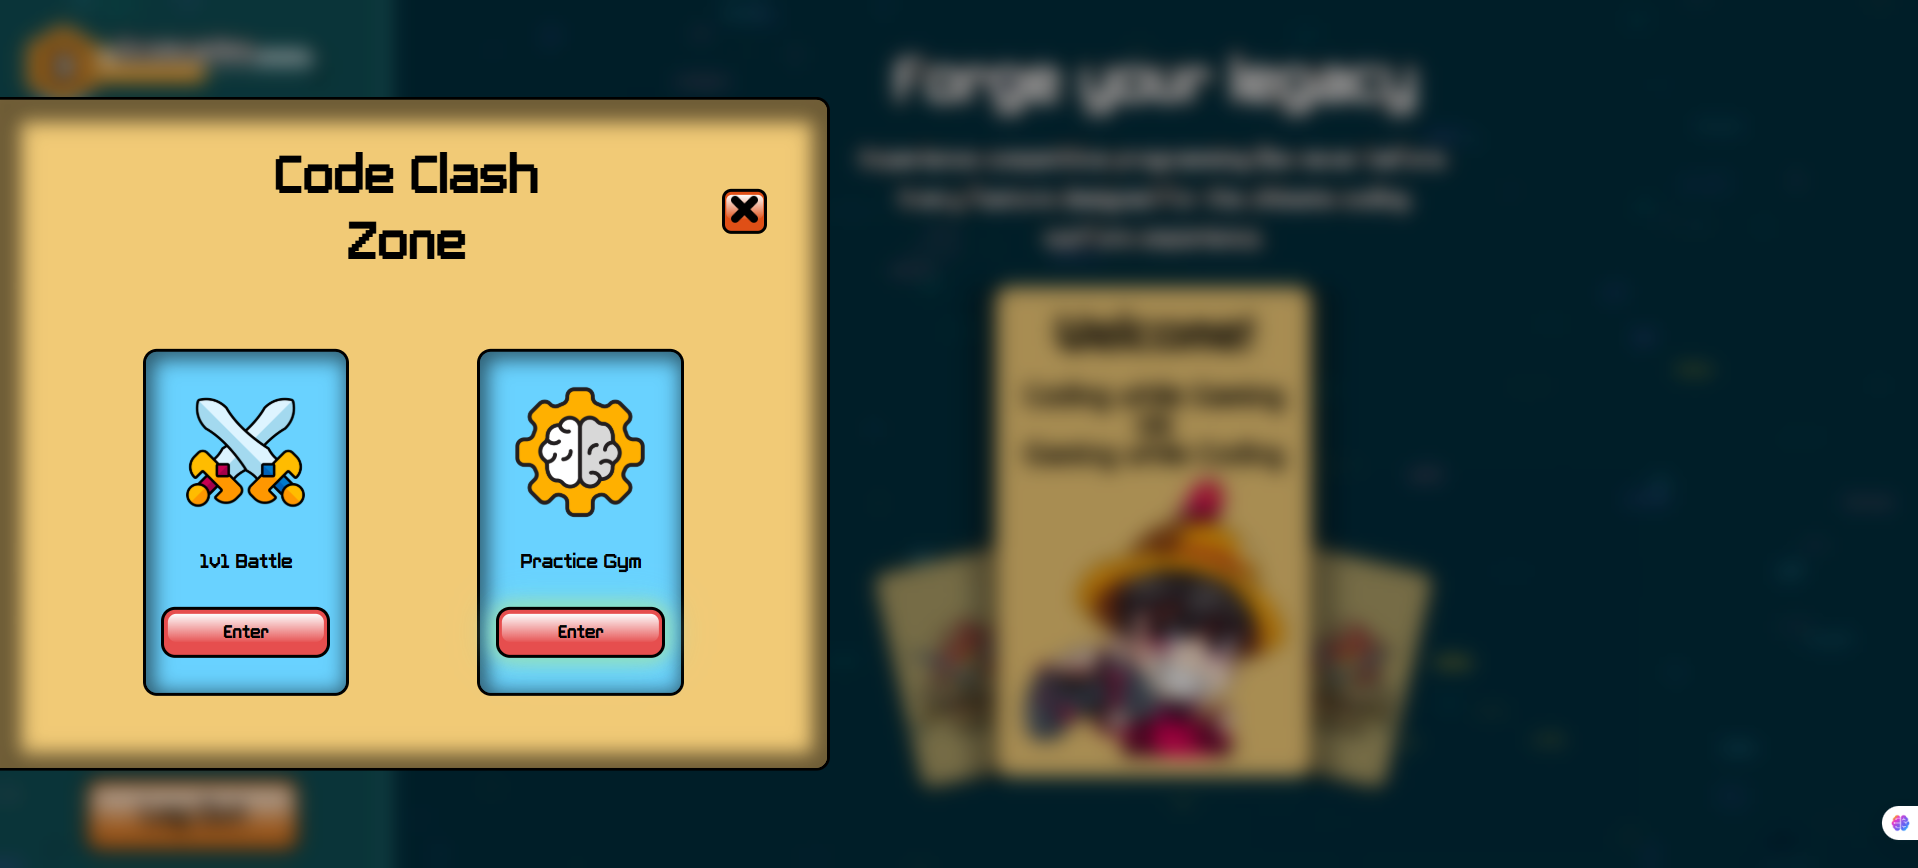
\includegraphics[width=0.9\textwidth]{select_practice_mode.png}
\caption{Battle Mode Selection - Practice Gym option}
\label{fig:practice_gym_select}
\end{figure}

\textbf{Step 2: Browse and Filter Problems}
\begin{enumerate}
\item The Practice Gym displays a list of available problems with filtering options:
  \begin{itemize}
    \item \textbf{Difficulty Filter}: Select rating range (e.g., 800-1000, 1200-1400, etc.)
    \item \textbf{Tag Filter}: Choose problem categories (e.g., Dynamic Programming, Graphs, Greedy, Math, etc.)
    \item \textbf{Search}: Search by problem name or contest ID
    \item \textbf{Solved Status}: Filter to show only unsolved problems or include solved
  \end{itemize}
\item Each problem displays:
  \begin{itemize}
    \item Problem name and ID (e.g., "1500A - Beautiful Numbers")
    \item Difficulty rating (e.g., 1200)
    \item Tags (e.g., "greedy, math")
    \item Solved status (checkmark if previously solved)
  \end{itemize}
\item Apply filters to narrow down problem selection
\item Browse through paginated problem list
\end{enumerate}

\begin{figure}[!htb]
\centering
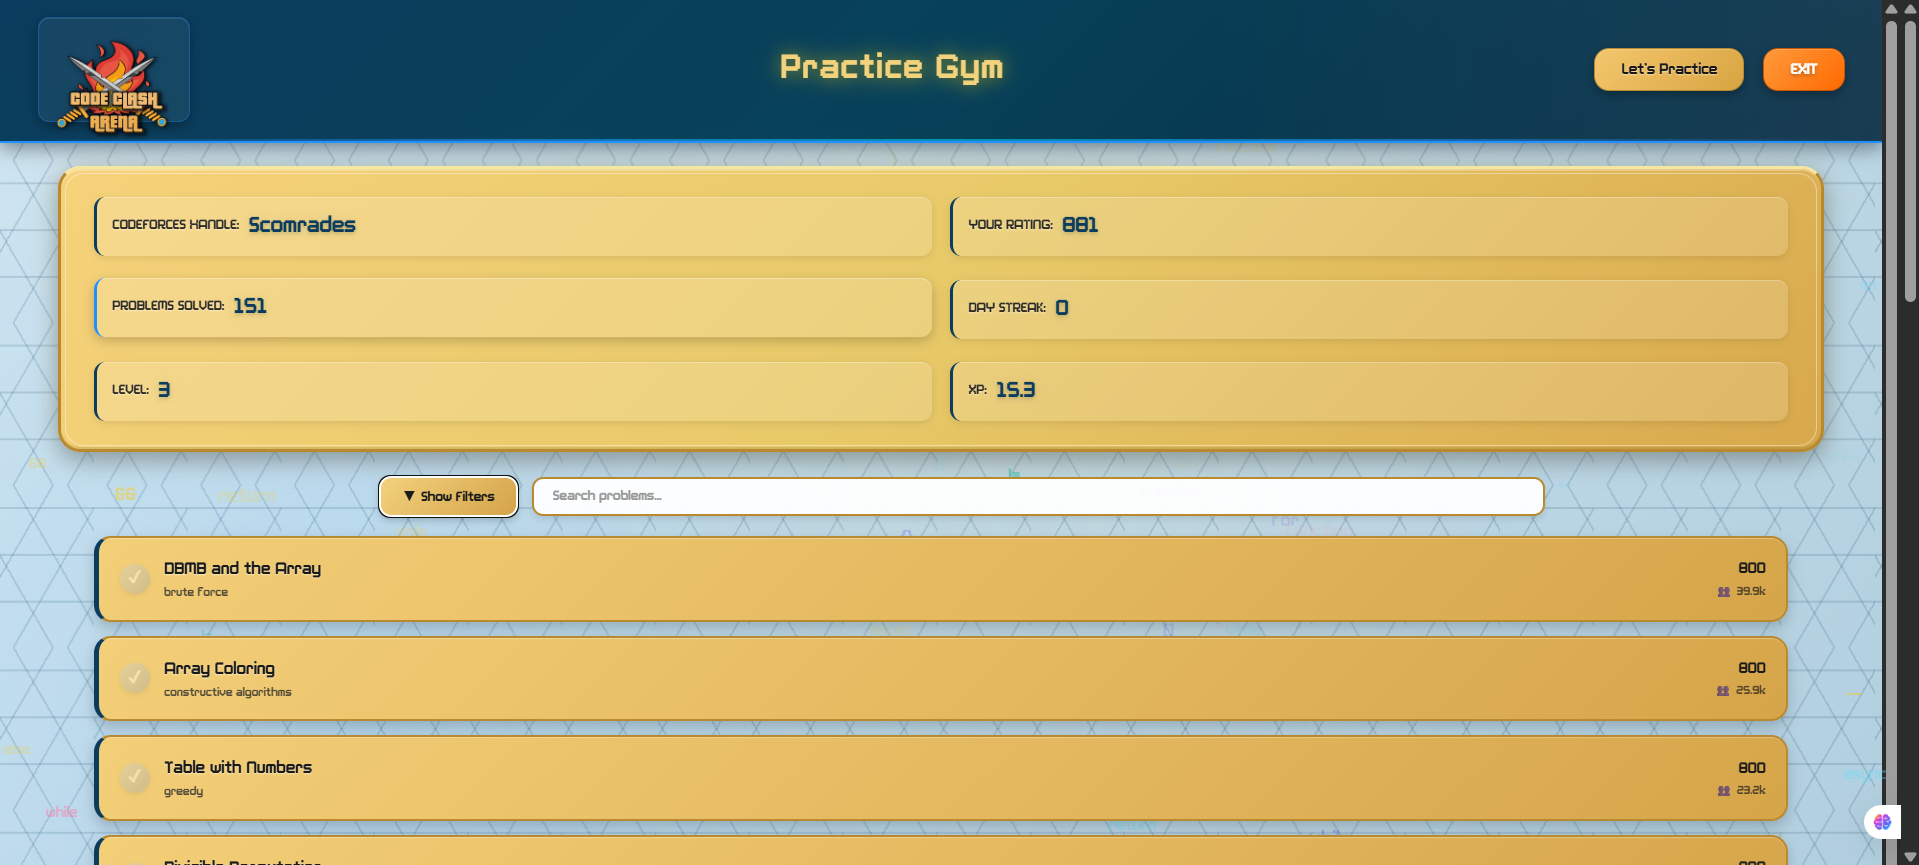
\includegraphics[width=0.9\textwidth]{practice_dashboard.png}
\caption{Practice Gym - Problem browser with filtering options}
\label{fig:practice_gym_browser}
\end{figure}

\textbf{Step 3: Select a Problem}
\begin{enumerate}
\item Click on a problem from the list to open it
\item Problem page loads with:
  \begin{itemize}
    \item Problem statement (Codeforces problem embedded in iframe or rendered text)
    \item Input/output specifications
    \item Sample test cases
    \item Constraints and notes
  \end{itemize}
\item Read the problem carefully
\item Analyze sample inputs and outputs
\item Click \textbf{"Start Solving"} or \textbf{"Open Editor"} to begin coding
\end{enumerate}

\begin{figure}[!htb]
\centering
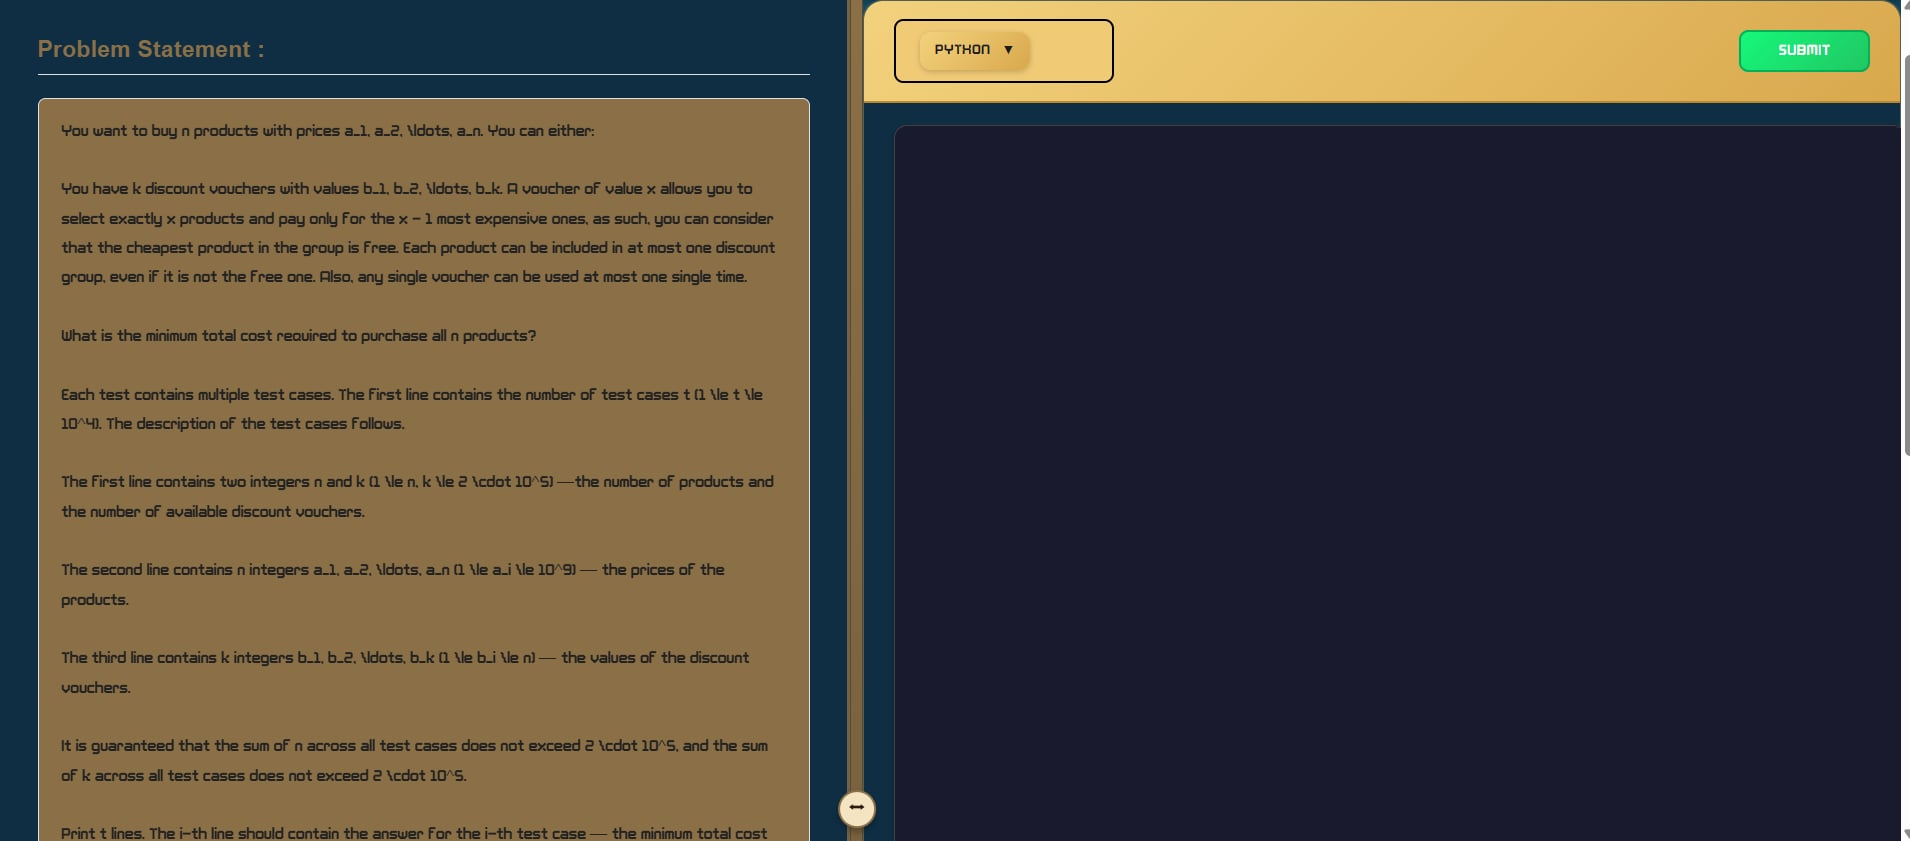
\includegraphics[width=0.9\textwidth]{practice_problem_statement.png}
\caption{Practice Gym - Problem statement display}
\label{fig:practice_problem_view}
\end{figure}

\textbf{Step 4: Solving the Problem}
\begin{enumerate}
\item Practice solving interface loads with:
  \begin{itemize}
    \item \textbf{Left Panel}: Problem statement (persistent view)
    \item \textbf{Right Panel}: Code editor
    \item \textbf{Top Bar}: Problem title, timer (optional), hint button
  \end{itemize}
\item Select programming language from dropdown
\item Write your solution code
\item No time limit - work at your own pace
\item Code editor supports syntax highlighting, auto-indentation, and basic autocomplete
\end{enumerate}

\textbf{Step 5: Local Testing}
\begin{enumerate}
\item Use the \textbf{"Run Code"} or \textbf{"Test"} button to test your solution locally
\item Input test cases:
  \begin{itemize}
    \item Use provided sample test cases (auto-populated)
    \item Or enter custom test cases manually
  \end{itemize}
\item Click \textbf{"Run"} to execute code
\item View output results:
  \begin{itemize}
    \item Expected output vs. your output
    \item Execution time
    \item Any runtime errors or compilation errors
  \end{itemize}
\item Debug and refine your solution based on test results
\item Run multiple tests with different inputs
\end{enumerate}

\textbf{Step 6: AI Hint System (Optional)}
\begin{enumerate}
\item If stuck on the problem, click the \textbf{"Get Hint"} button (lightbulb icon)
\item AI hint system provides logical guidance without revealing full solution:
  \begin{itemize}
    \item Hint Level 1: General approach or algorithm category (e.g., "Consider using a greedy approach")
    \item Hint Level 2: More specific guidance (e.g., "Sort the array first, then iterate")
    \item Hint Level 3: Detailed steps without code (e.g., "Maintain two pointers...")
  \end{itemize}
\item Hints are progressive - start with Level 1, request more if needed
\item Each hint displays in a popup or side panel
\item Use hints to learn problem-solving strategies
\end{enumerate}

\begin{figure}[!htb]
\centering
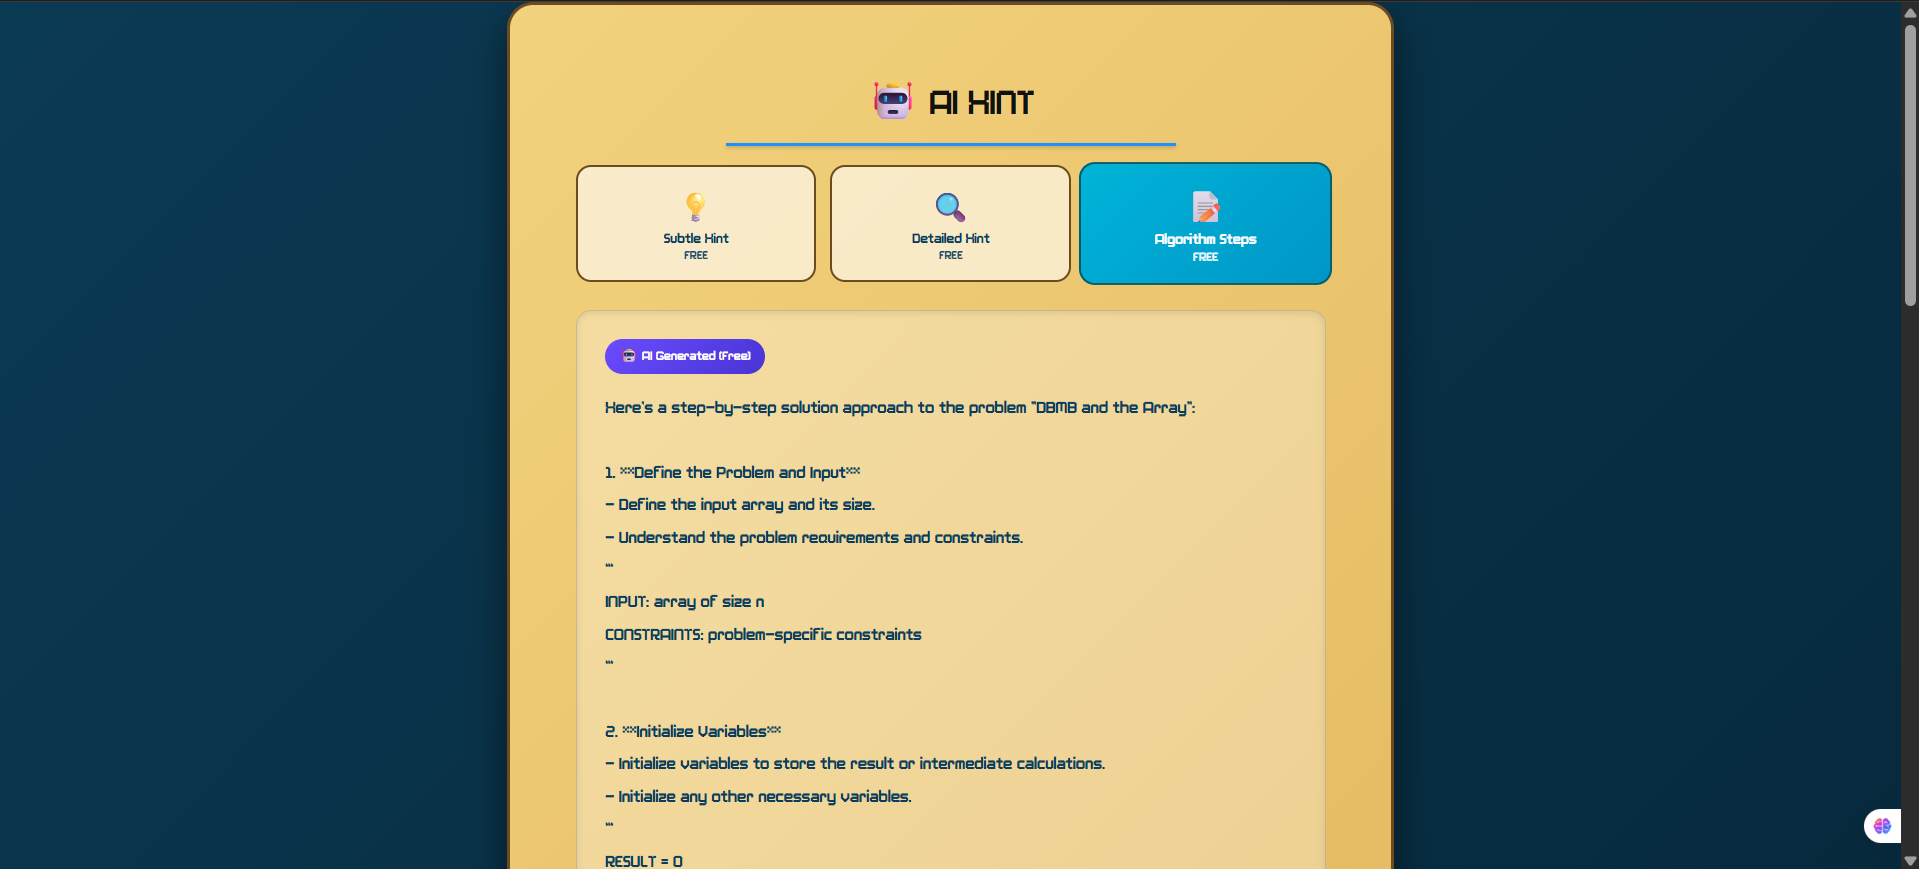
\includegraphics[width=0.9\textwidth]{AI_hint.png}
\caption{Practice Gym - AI hint system}
\label{fig:practice_hints}
\end{figure}

\textbf{Step 7: Submit Solution}
\begin{enumerate}
\item Once confident in your solution, click \textbf{"Submit"} button
\item Code is submitted to Codeforces judge for official evaluation
\item Verdict process (same as battle mode):
  \begin{itemize}
    \item "Submitting..." → "In Queue" → "Running on Test X"
    \item Final verdict: Accepted, Wrong Answer, TLE, RE, CE, etc.
  \end{itemize}
\item If Accepted:
  \begin{itemize}
    \item Success notification: "Problem Solved!"
    \item XP is awarded (less than battle mode, but still contributes to progression)
    \item Problem marked as solved in your profile
    \item Checkmark appears next to problem in problem list
  \end{itemize}
\item If not Accepted:
  \begin{itemize}
    \item Review verdict and failed test case (if available)
    \item Modify code and resubmit
    \item Unlimited submission attempts
  \end{itemize}
\end{enumerate}

\textbf{Step 8: Return to Problem Browser}
\begin{enumerate}
\item After solving (or at any time), click \textbf{"Back to Problems"} or \textbf{"Exit"} button
\item Return to Practice Gym problem browser
\item Solved problem now shows checkmark indicator
\item Statistics updated: total problems solved, difficulty distribution
\item Select another problem to continue practicing
\end{enumerate}

\textbf{Input Requirements:}
\begin{itemize}[leftmargin=*]
\item \textbf{Problem Selection}: Choose difficulty range, tags, or specific problem
\item \textbf{Code Input}: Solution code in selected language
\item \textbf{Test Input}: Sample or custom test cases for local testing
\item \textbf{Hint Request}: Optional - request AI assistance
\end{itemize}

\textbf{Output and Results:}
\begin{itemize}[leftmargin=*]
\item \textbf{Problem List Output}: Filtered problems matching criteria, difficulty ratings, tags
\item \textbf{Local Test Output}: Execution results, output comparison, runtime
\item \textbf{Hint Output}: AI-generated logical guidance (progressive levels)
\item \textbf{Submission Output}: Official Codeforces verdict, XP earned (if Accepted), solved status update
\item \textbf{Statistics Output}: Updated solve count, progress tracking
\end{itemize}

\textbf{Special Features:}
\begin{itemize}[leftmargin=*]
\item \textbf{No Time Pressure}: Learn and practice at your own pace
\item \textbf{AI Hints}: Intelligent guidance system for learning
\item \textbf{Extensive Problem Library}: Access to thousands of Codeforces problems
\item \textbf{Progress Tracking}: Monitor which problems you've solved
\item \textbf{Local Testing}: Test code before submission without penalty
\item \textbf{XP Rewards}: Earn experience points for skill progression
\end{itemize}

\FloatBarrier

% ==================================================
\subsection{Clan System}

The Clan System enables team-based competitive coding through collaborative clans. Users can create clans, recruit members, and participate in clan battles where teams compete for points and rankings.

\subsubsection{Creating and Joining Clans}

\textbf{Purpose:} Form or join coding teams to participate in clan wars, collaborate with teammates, and compete for clan rankings and glory.

\textbf{Creating a New Clan:}

\textbf{Step 1: Access Clan Interface}
\begin{enumerate}
\item From Main Dashboard, click \textbf{"Your Clan"} button on the left navigation menu
\item If you are not in a clan, the clan browsing menu appears
\item Interface shows options: \textbf{"Create Clan"}, \textbf{"Find Clan"}, and list of available clans
\end{enumerate}

\begin{figure}[!htb]
\centering
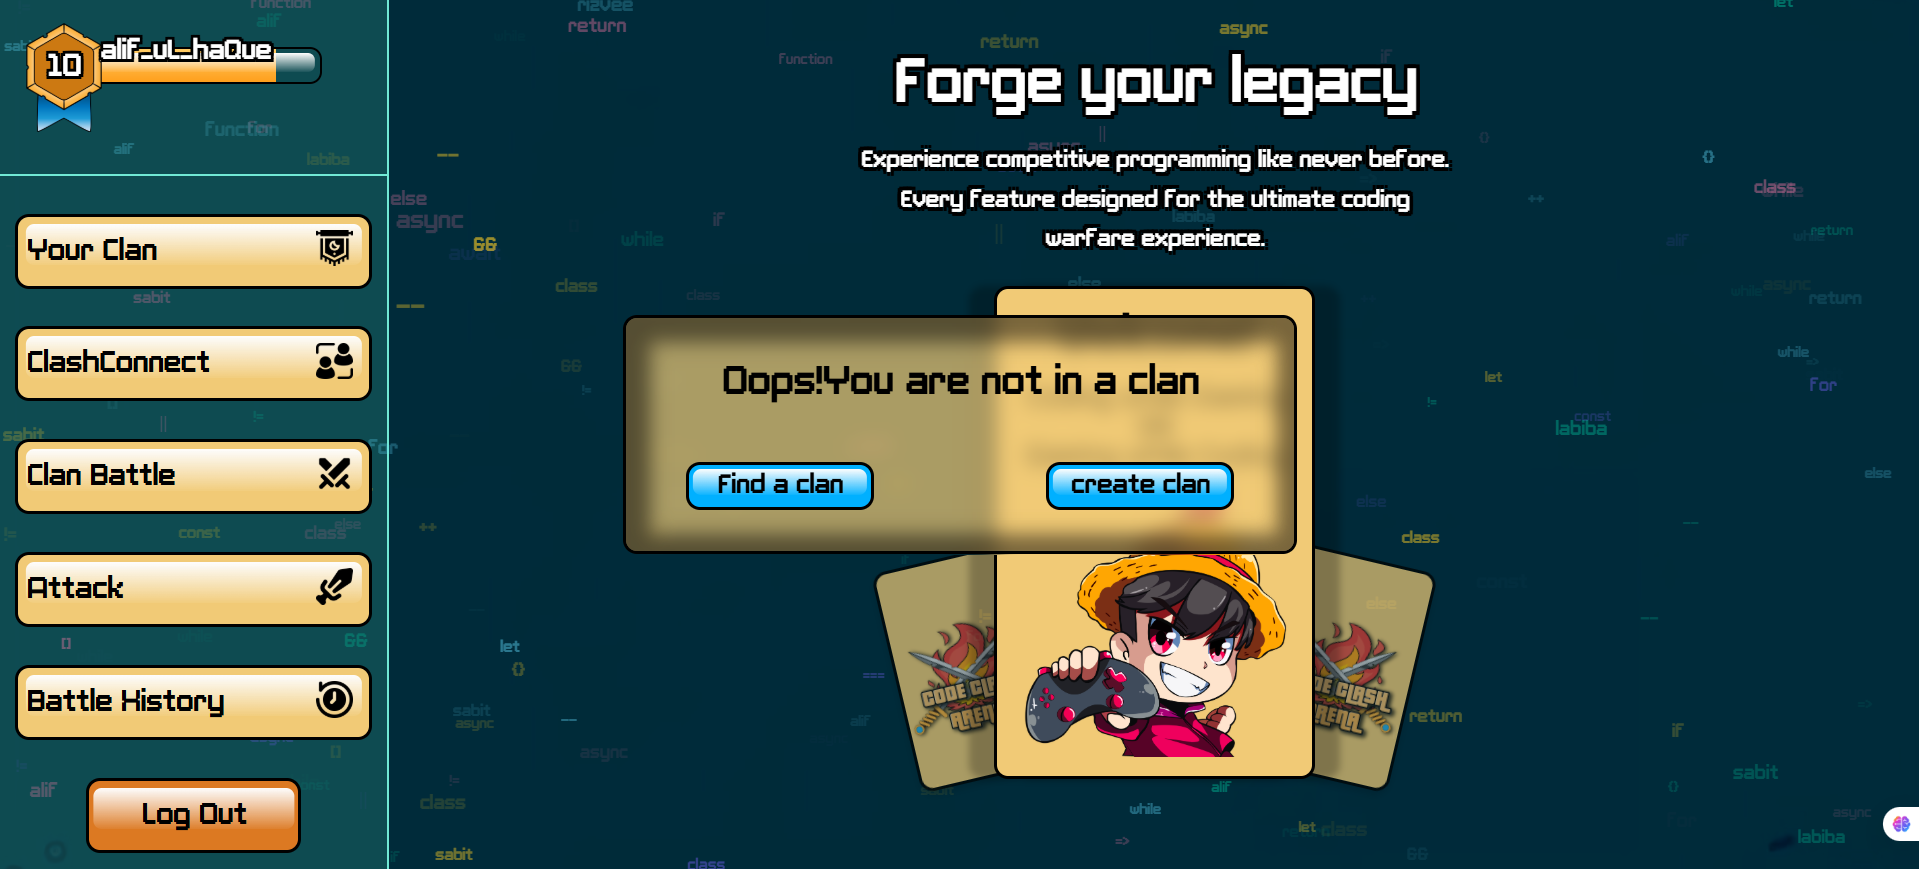
\includegraphics[width=0.9\textwidth]{create_or_join_clan.png}
\caption{Clan Menu - Create or Join options for users without clan}
\label{fig:clan_menu_no_clan}
\end{figure}

\textbf{Step 2: Initiate Clan Creation}
\begin{enumerate}
\item Click the \textbf{"Create Clan"} button
\item Clan creation form appears with required fields
\end{enumerate}

\textbf{Step 3: Fill Clan Information}
\begin{enumerate}
\item Enter clan details in the creation form:
  \begin{itemize}
    \item \textbf{Clan Name}: Unique name for your clan (3-30 characters, alphanumeric)
    \item \textbf{Clan Tag}: Short identifier (2-5 characters, appears in brackets, e.g., [TAG])
    \item \textbf{Description}: Brief description of clan (optional, up to 200 characters)
    \item \textbf{Clan Type}: Public (anyone can request to join) or Private (invite-only)
    \item \textbf{Member Limit}: Maximum members allowed (typically 10-50)
    \item \textbf{Minimum Rating}: Required rating for joining (optional filter)
  \end{itemize}
\item Review all information
\item Click \textbf{"Create Clan"} button to finalize
\end{enumerate}

\begin{figure}[!htb]
\centering
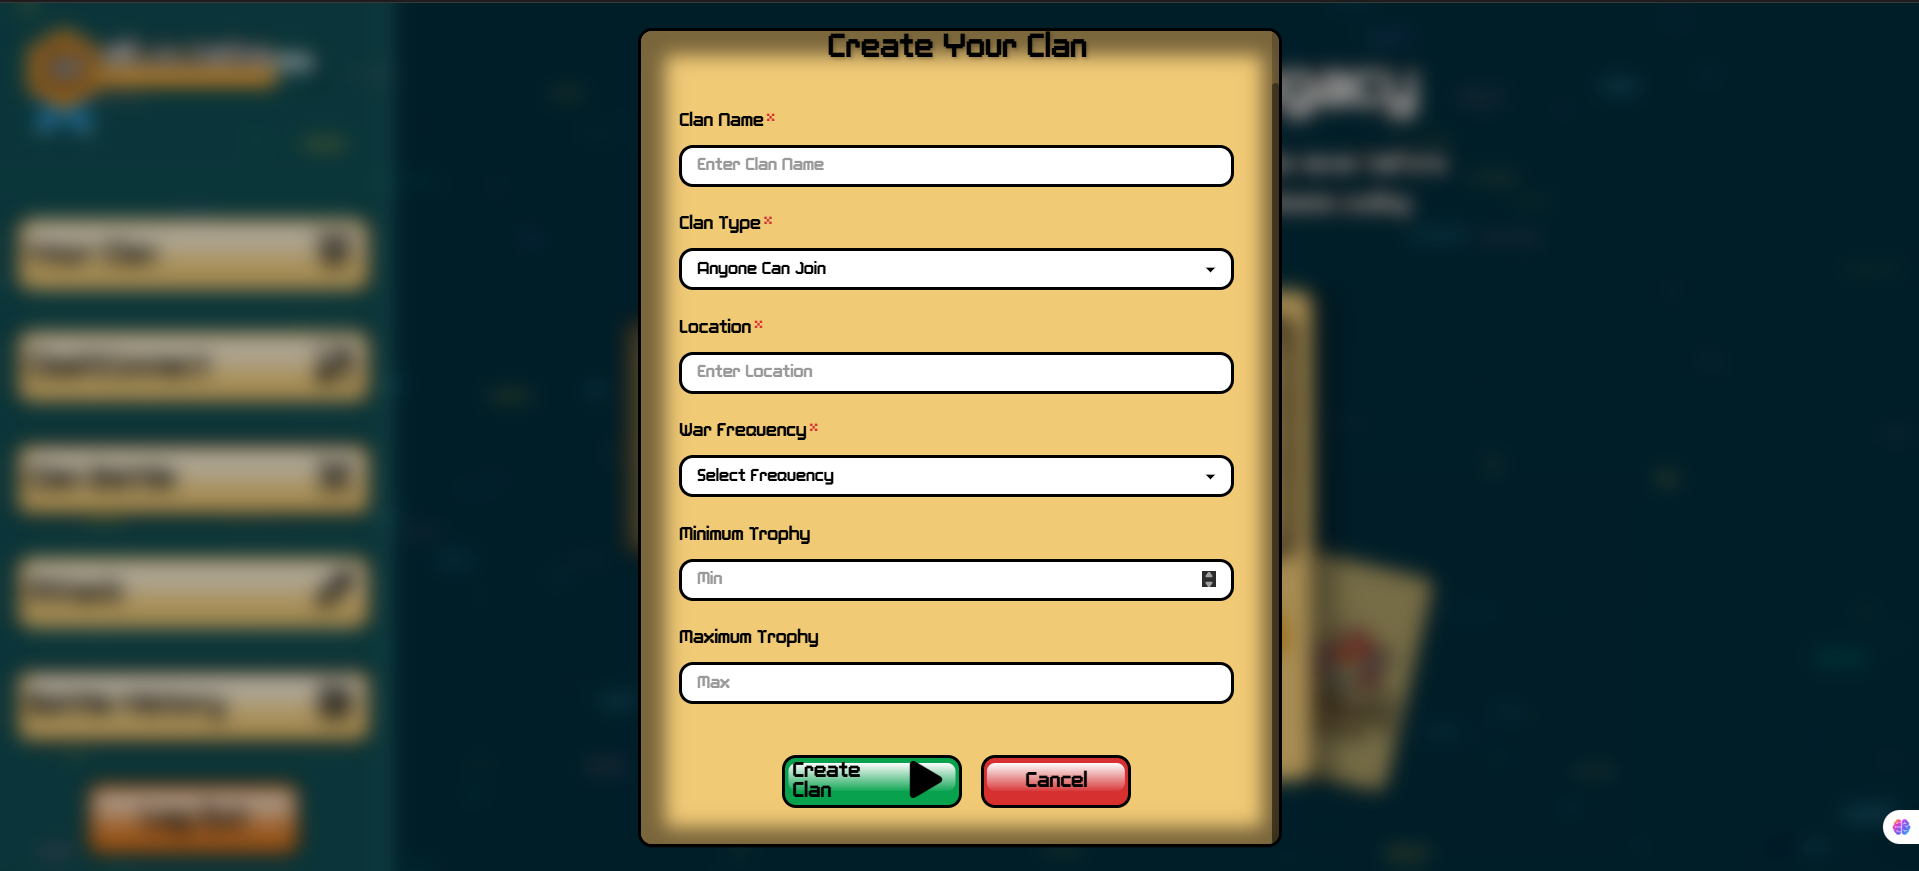
\includegraphics[width=0.9\textwidth]{clan_create_form.png}
\caption{Clan Creation - Form with all required fields}
\label{fig:clan_creation_form}
\end{figure}

\textbf{Step 4: Clan Created Successfully}
\begin{enumerate}
\item Success notification: "Clan created successfully!"
\item You are automatically set as Clan Leader
\item Redirected to your clan's main page showing:
  \begin{itemize}
    \item Clan name, tag, and description
    \item Member list (currently only you)
    \item Clan statistics: Total points (0), battles fought (0), wins/losses
    \item Join requests section (empty initially)
  \end{itemize}
\item Clan is now visible to other users in clan browsing list
\end{enumerate}

\begin{figure}[!htb]
\centering
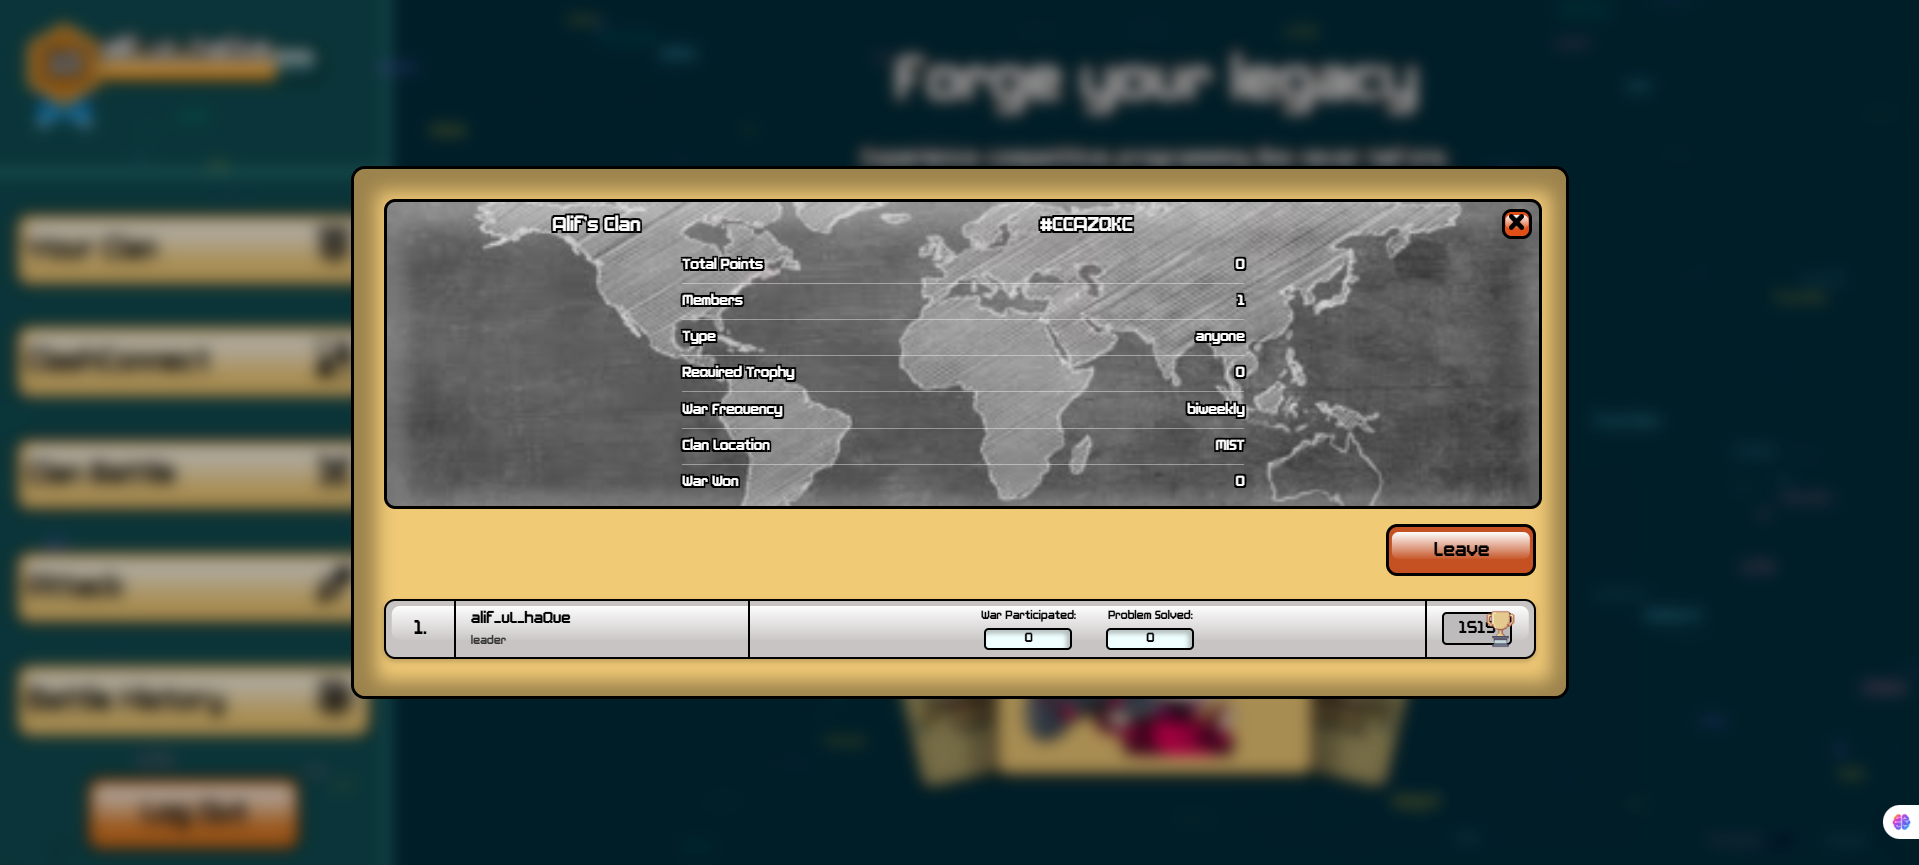
\includegraphics[width=0.9\textwidth]{newly_formed_clan.png}
\caption{New Clan Page - Clan leader view after creation}
\label{fig:new_clan_page}
\end{figure}

\textbf{Joining an Existing Clan:}

\textbf{Step 1: Browse Available Clans}
\begin{enumerate}
\item From the clan menu (accessed via "Your Clan" button), click \textbf{"Find Clan"}
\item List of public clans displays with details:
  \begin{itemize}
    \item Clan name and tag
    \item Member count (e.g., "15/30 members")
    \item Clan rating/points
    \item Description summary
    \item Minimum rating requirement
  \end{itemize}
\item Use search/filter options to find specific clans:
  \begin{itemize}
    \item Search by clan name
    \item Filter by rating requirement
    \item Sort by clan points or member count
  \end{itemize}
\end{enumerate}

\begin{figure}[!htb]
\centering
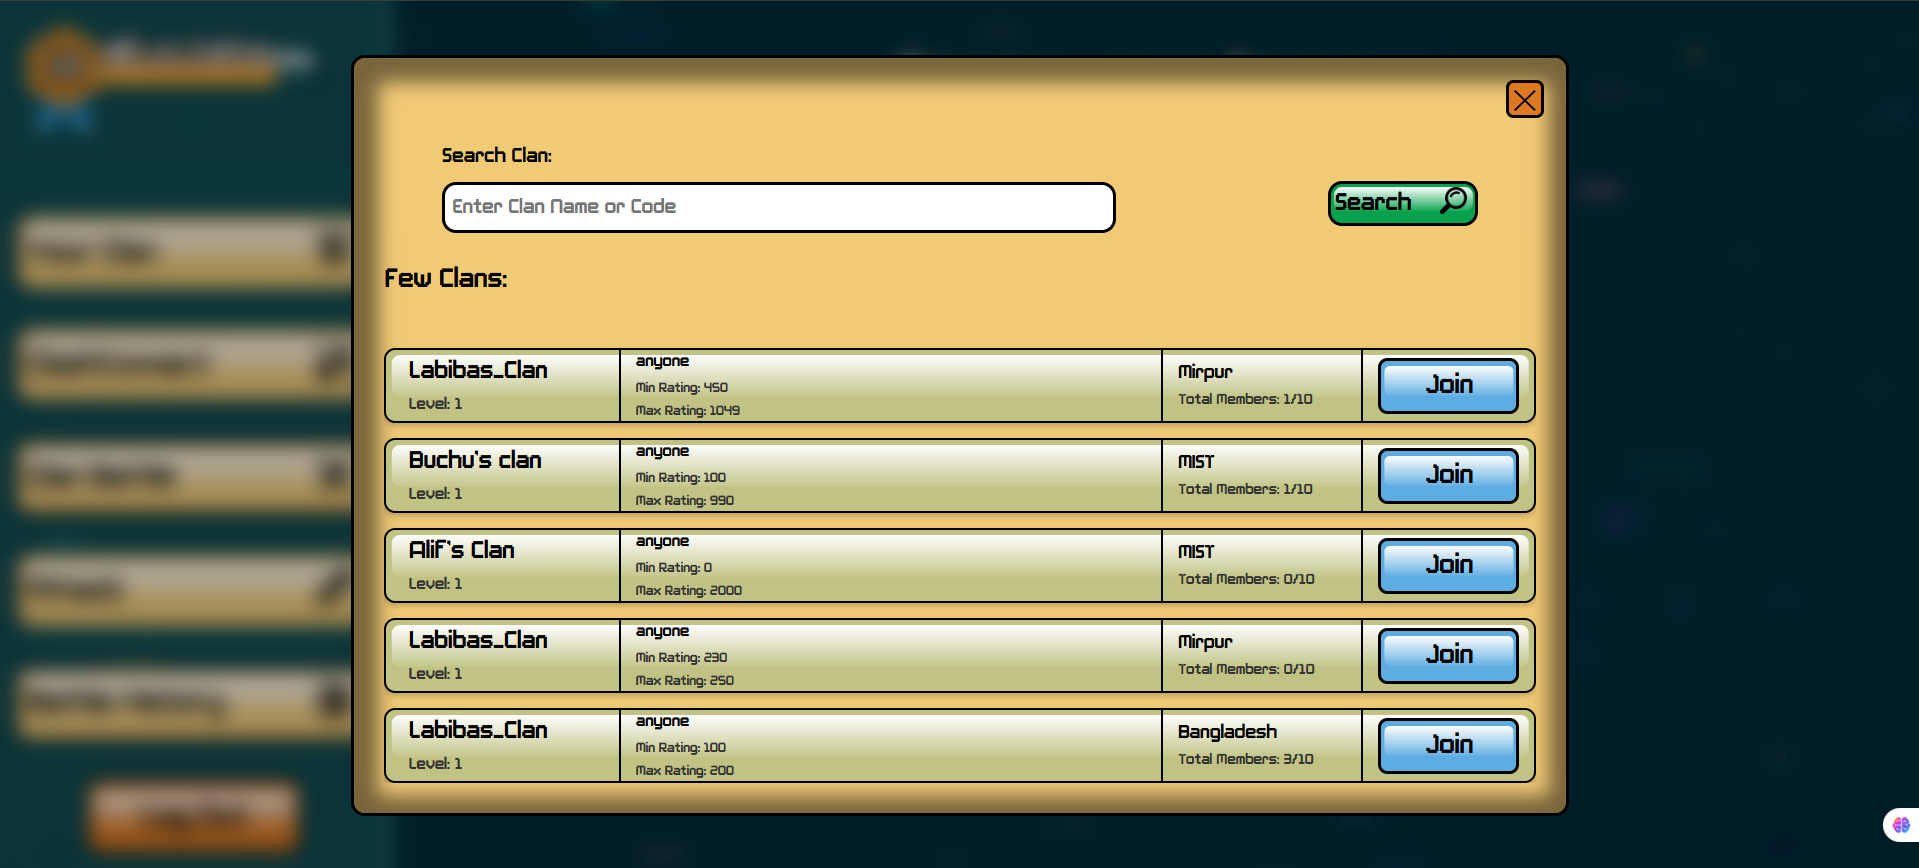
\includegraphics[width=0.9\textwidth]{join_clan.png}
\caption{Clan Browser - List of available clans to join}
\label{fig:clan_browser}
\end{figure}

\textbf{Step 2: Select and Request to Join}
\begin{enumerate}
\item Click on a clan to view full details
\item Clan detail page shows:
  \begin{itemize}
    \item Complete clan information
    \item Member list with usernames and ratings
    \item Recent battle history
    \item Clan statistics
  \end{itemize}
\item If you meet requirements, \textbf{"Request to Join"} button is enabled
\item Click \textbf{"Request to Join"} button
\item Confirmation message: "Join request sent to [Clan Name]"
\end{enumerate}

\begin{figure}[!htb]
\centering
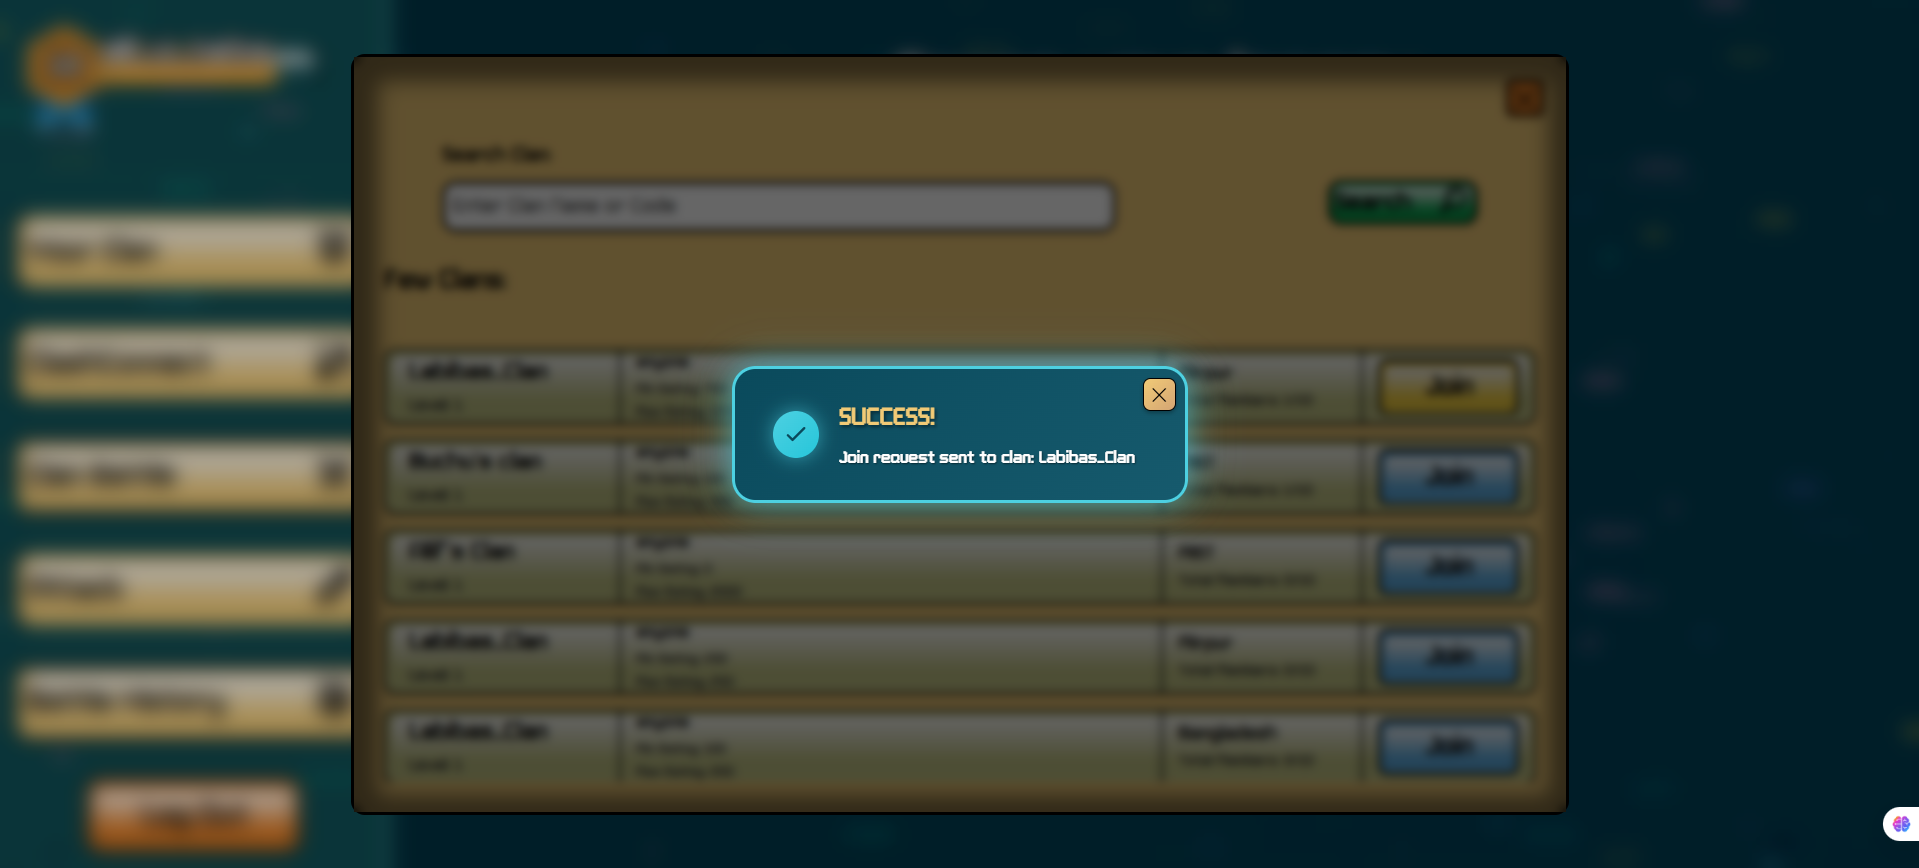
\includegraphics[width=0.9\textwidth]{clan_join_request_sent.png}
\caption{Clan Details - Request to join a clan}
\label{fig:clan_request_join}
\end{figure}

\textbf{Step 3: Wait for Approval}
\begin{enumerate}
\item Your join request is sent to the clan leader
\item Status shows: "Pending Approval"
\item Clan leader receives notification of your request
\item Leader can view your profile, rating, and statistics
\item Leader approves or rejects your request
\end{enumerate}

\textbf{Step 4: Join Request Accepted}
\begin{enumerate}
\item When leader approves, you receive notification: "You have been accepted to [Clan Name]!"
\item Click notification or navigate to "Your Clan"
\item Your clan page now displays:
  \begin{itemize}
    \item Clan information
    \item Full member list (including yourself)
    \item Clan chat/communication features
    \item Clan battle schedule
  \end{itemize}
\item You can now participate in clan battles when selected by leader
\end{enumerate}

\begin{figure}[!htb]
\centering
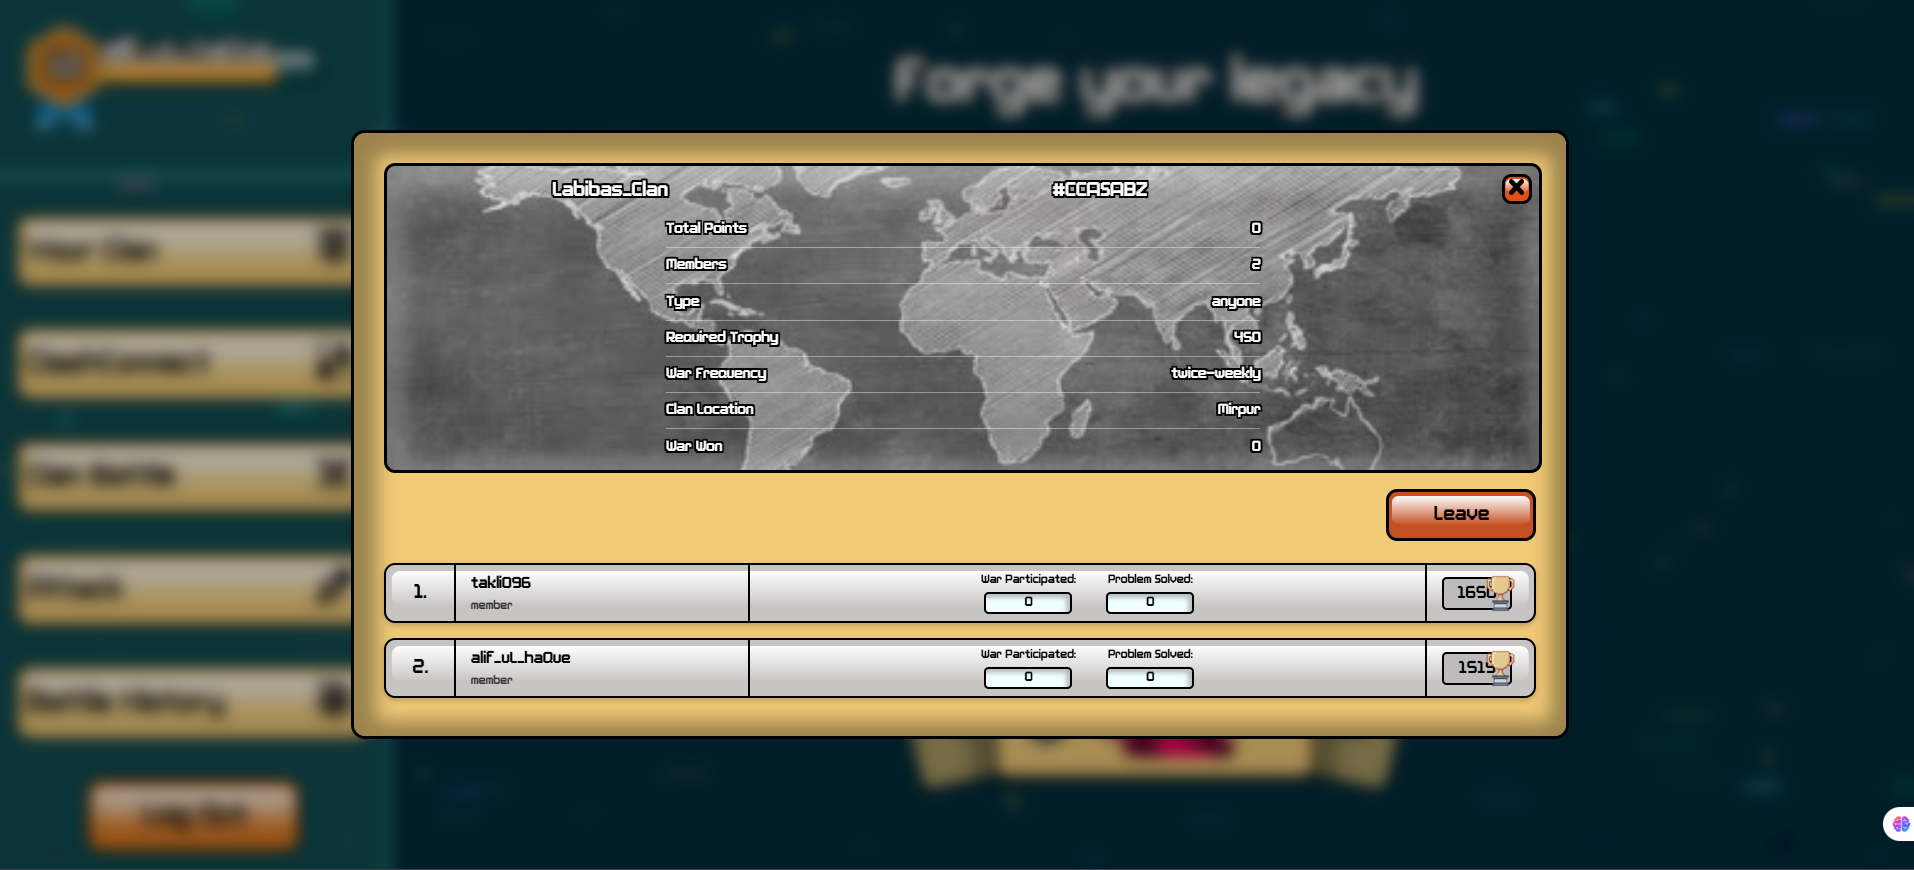
\includegraphics[width=0.9\textwidth]{clan_members.png}
\caption{Your Clan Page - Member view after joining}
\label{fig:clan_member_view}
\end{figure}

\textbf{Clan Leader Functions:}

If you are a clan leader, additional management options are available:

\begin{enumerate}
\item \textbf{Managing Join Requests}:
  \begin{itemize}
    \item Navigate to \textbf{"ClashConnect"} or check notifications
    \item View pending join requests with applicant details
    \item Click \textbf{"Accept"} to approve or \textbf{"Reject"} to deny
  \end{itemize}
\item \textbf{Managing Members}:
  \begin{itemize}
    \item View full member list in clan page
    \item Option to \textbf{"Remove Member"} (kick from clan)
    \item Promote members to co-leader (if feature available)
  \end{itemize}
\item \textbf{Initiating Clan Battles}:
  \begin{itemize}
    \item Select warriors for upcoming battles
    \item Start matchmaking for clan wars
    \item(Detailed in next subsection)
  \end{itemize}
\item \textbf{Edit Clan Settings}:
  \begin{itemize}
    \item Update description, logo, or settings
    \item Change clan type (public/private)
    \item Adjust member limit or rating requirements
  \end{itemize}
\end{enumerate}

\begin{figure}[!htb]
\centering
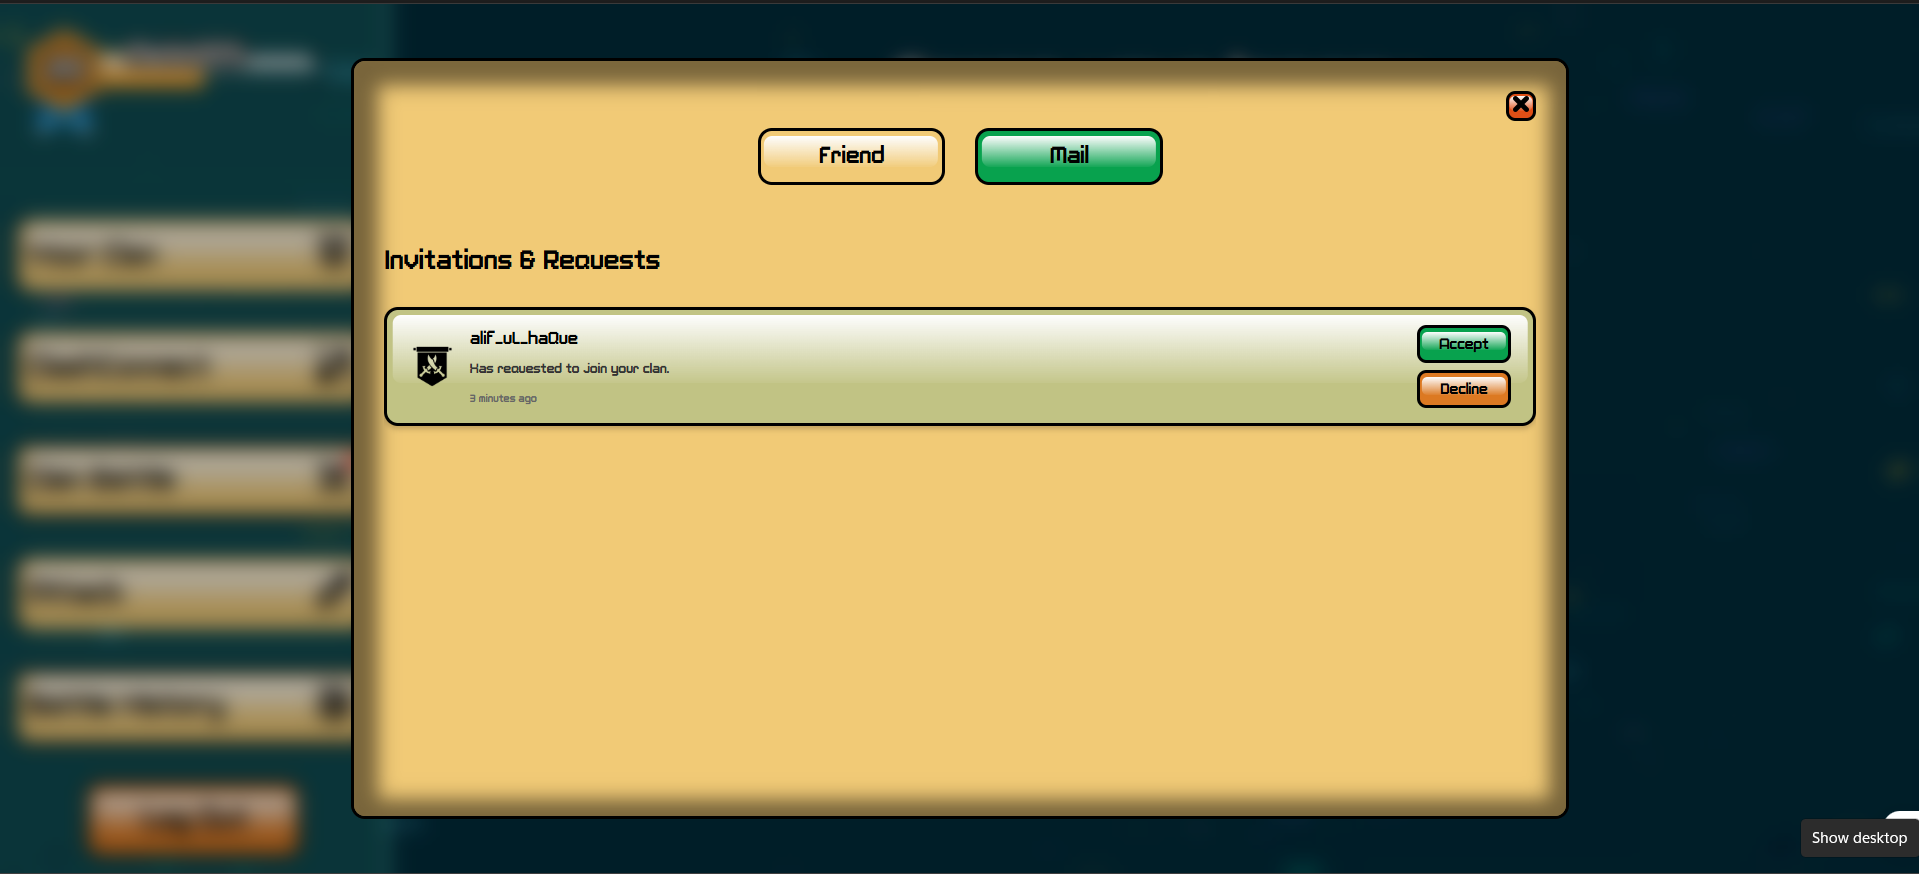
\includegraphics[width=0.9\textwidth]{incoming_clan_join_request.png}
\caption{Clan Leader Interface - Managing requests and members}
\label{fig:clan_leader_management}
\end{figure}

\textbf{Leaving a Clan:}

\begin{enumerate}
\item From your clan page, locate \textbf{"Leave Clan"} button (typically at bottom or in settings)
\item Click \textbf{"Leave Clan"}
\item Confirmation dialog: "Are you sure you want to leave [Clan Name]?"
\item Click \textbf{"Confirm"} to leave
\item Success message: "You have left the clan"
\item Redirected to clan browsing menu
\item Note: If you are the leader, you must transfer leadership or disband clan first
\end{enumerate}

\textbf{Input Requirements:}
\begin{itemize}[leftmargin=*]
\item \textbf{Creating Clan}: Clan name (unique), tag, description, type, member limit, minimum rating
\item \textbf{Joining Clan}: Must meet clan's rating requirement (if any), cannot be in another clan
\item \textbf{Leader Actions}: Select members for battles, approve/reject requests
\end{itemize}

\textbf{Output and Results:}
\begin{itemize}[leftmargin=*]
\item \textbf{Clan Creation Output}: New clan created with you as leader, clan visible in browser
\item \textbf{Join Request Output}: Request sent to leader, pending status
\item \textbf{Membership Output}: Access to clan page, chat, battles, statistics
\item \textbf{Management Output}: Notifications for join requests, member updates
\end{itemize}

\FloatBarrier

\subsubsection{Clan Battles}

\textbf{Purpose:} Participate in team-based coding competitions where clans compete against each other. Selected clan members solve problems to earn points for their clan, with cumulative scores determining the winning team.

\textbf{Step-by-Step Usage (Clan Leader):}

\textbf{Step 1: Access Clan Battle Interface}
\begin{enumerate}
\item From Main Dashboard, click \textbf{"Clan Battle"} button on left navigation
\item As clan leader, you are taken to the warrior selection page
\item Page displays list of all clan members with their ratings and availability
\end{enumerate}

\begin{figure}[!htb]
\centering
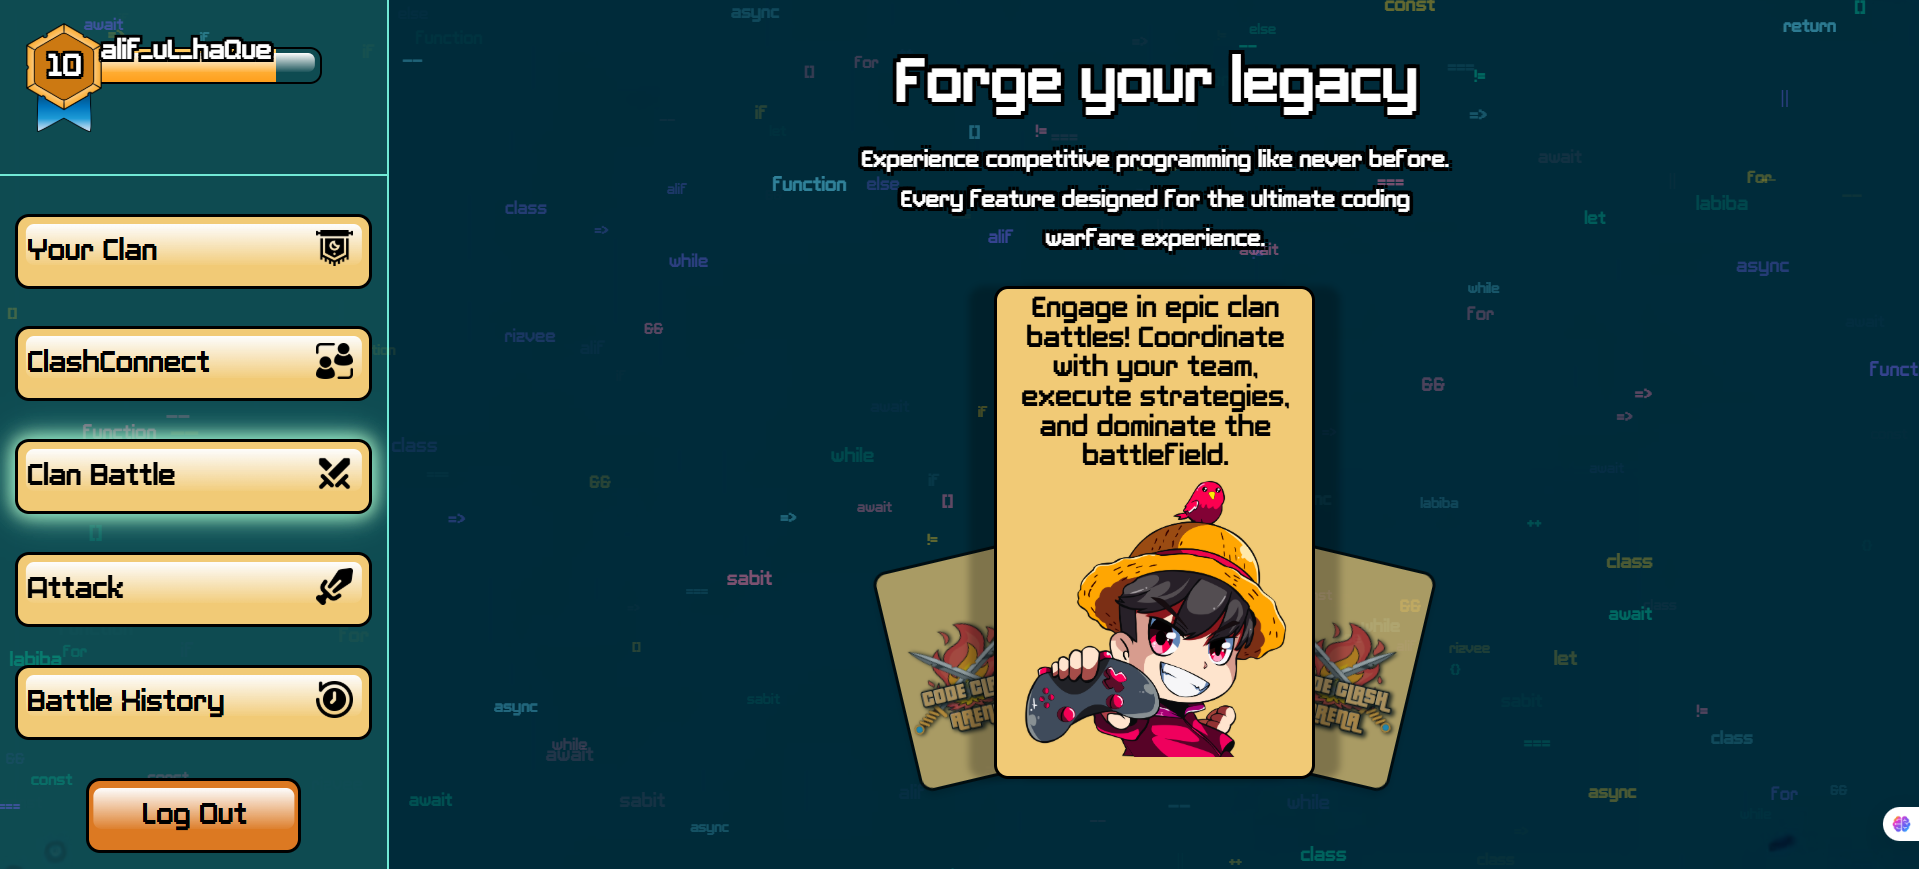
\includegraphics[width=0.9\textwidth]{select_clan_battle.png}
\caption{Main Dashboard - Clan Battle access}
\label{fig:clan_battle_access}
\end{figure}

\textbf{Step 2: Select Warriors}
\begin{enumerate}
\item Choose members to participate in the clan battle:
  \begin{itemize}
    \item Typically 3-5 warriors per battle (varies by system configuration)
    \item Click on member names to select/deselect
    \item Selected members are highlighted
    \item Member ratings displayed to help make strategic selections
  \end{itemize}
\item Review selected warriors
\item Click \textbf{"Confirm Selection"} or \textbf{"Ready for Battle"} button
\end{enumerate}

\begin{figure}[!htb]
\centering
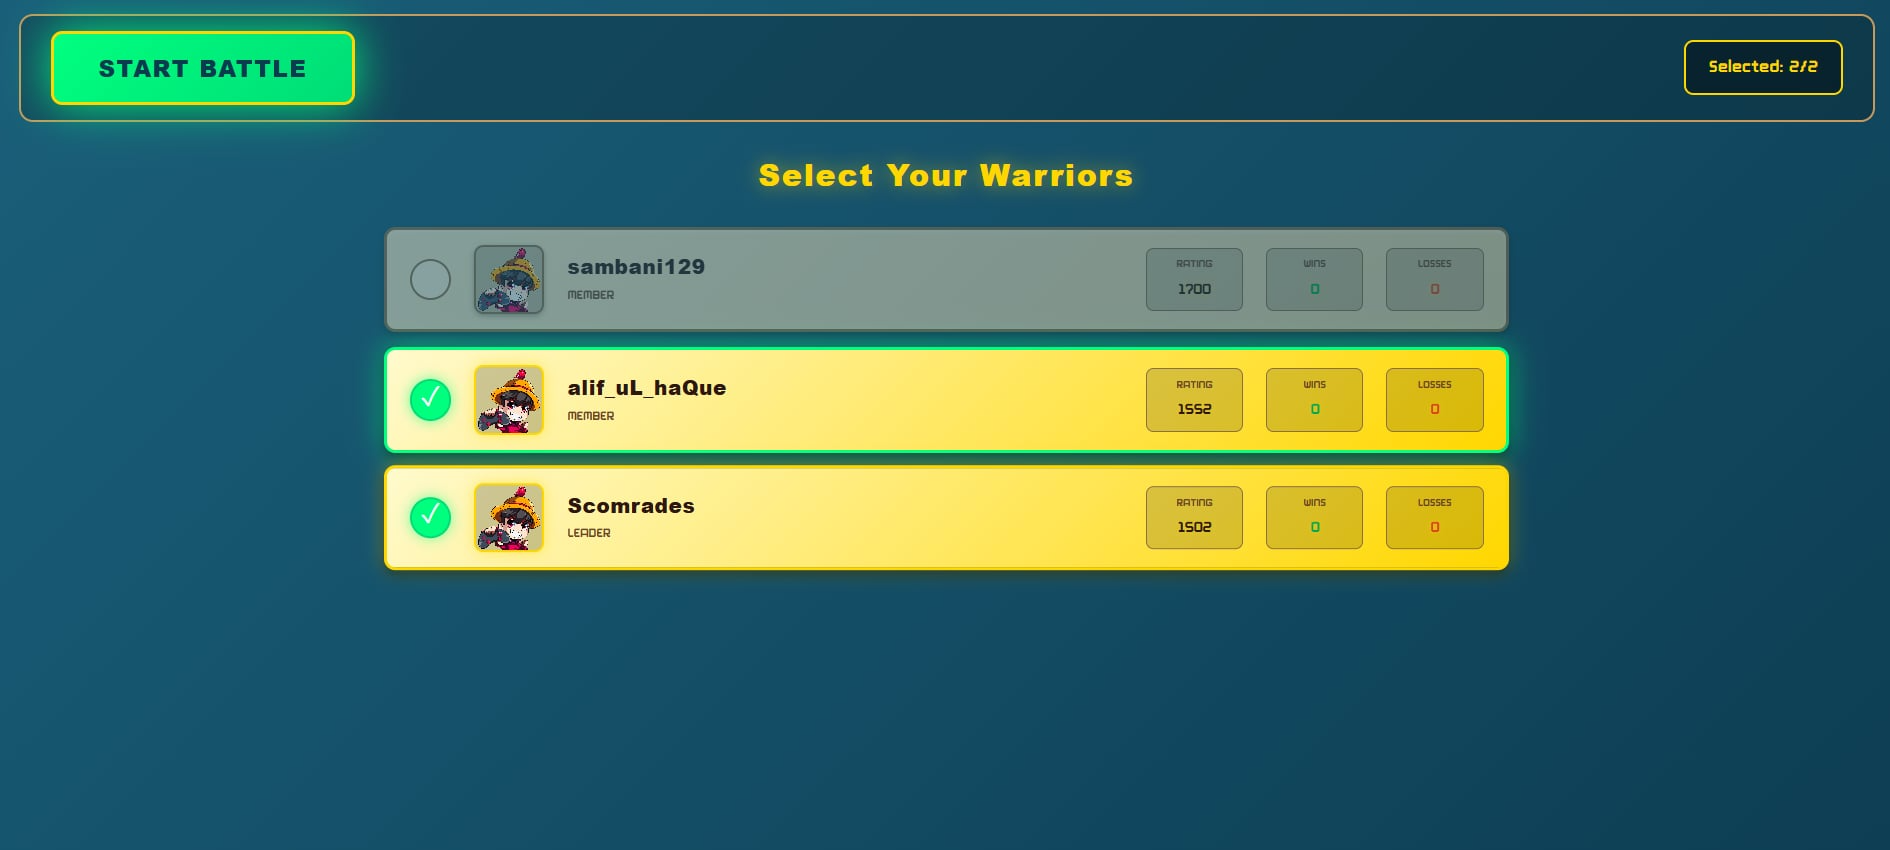
\includegraphics[width=0.9\textwidth]{warrior_selection.png}
\caption{Clan Battle - Warrior selection by leader}
\label{fig:warrior_selection}
\end{figure}

\textbf{Step 3: Initiate Matchmaking}
\begin{enumerate}
\item After confirming warrior selection, click \textbf{"Find Opponent Clan"} or \textbf{"Start Matchmaking"}
\item System searches for another clan ready for battle with similar:
  \begin{itemize}
    \item Clan rating
    \item Number of warriors
    \item Battle tier
  \end{itemize}
\item Searching status displays: "Searching for opponent clan..."
\item Matchmaking may take 30 seconds to several minutes depending on availability
\item You can cancel matchmaking by clicking \textbf{"Cancel Search"}
\end{enumerate}

\begin{figure}[!htb]
\centering
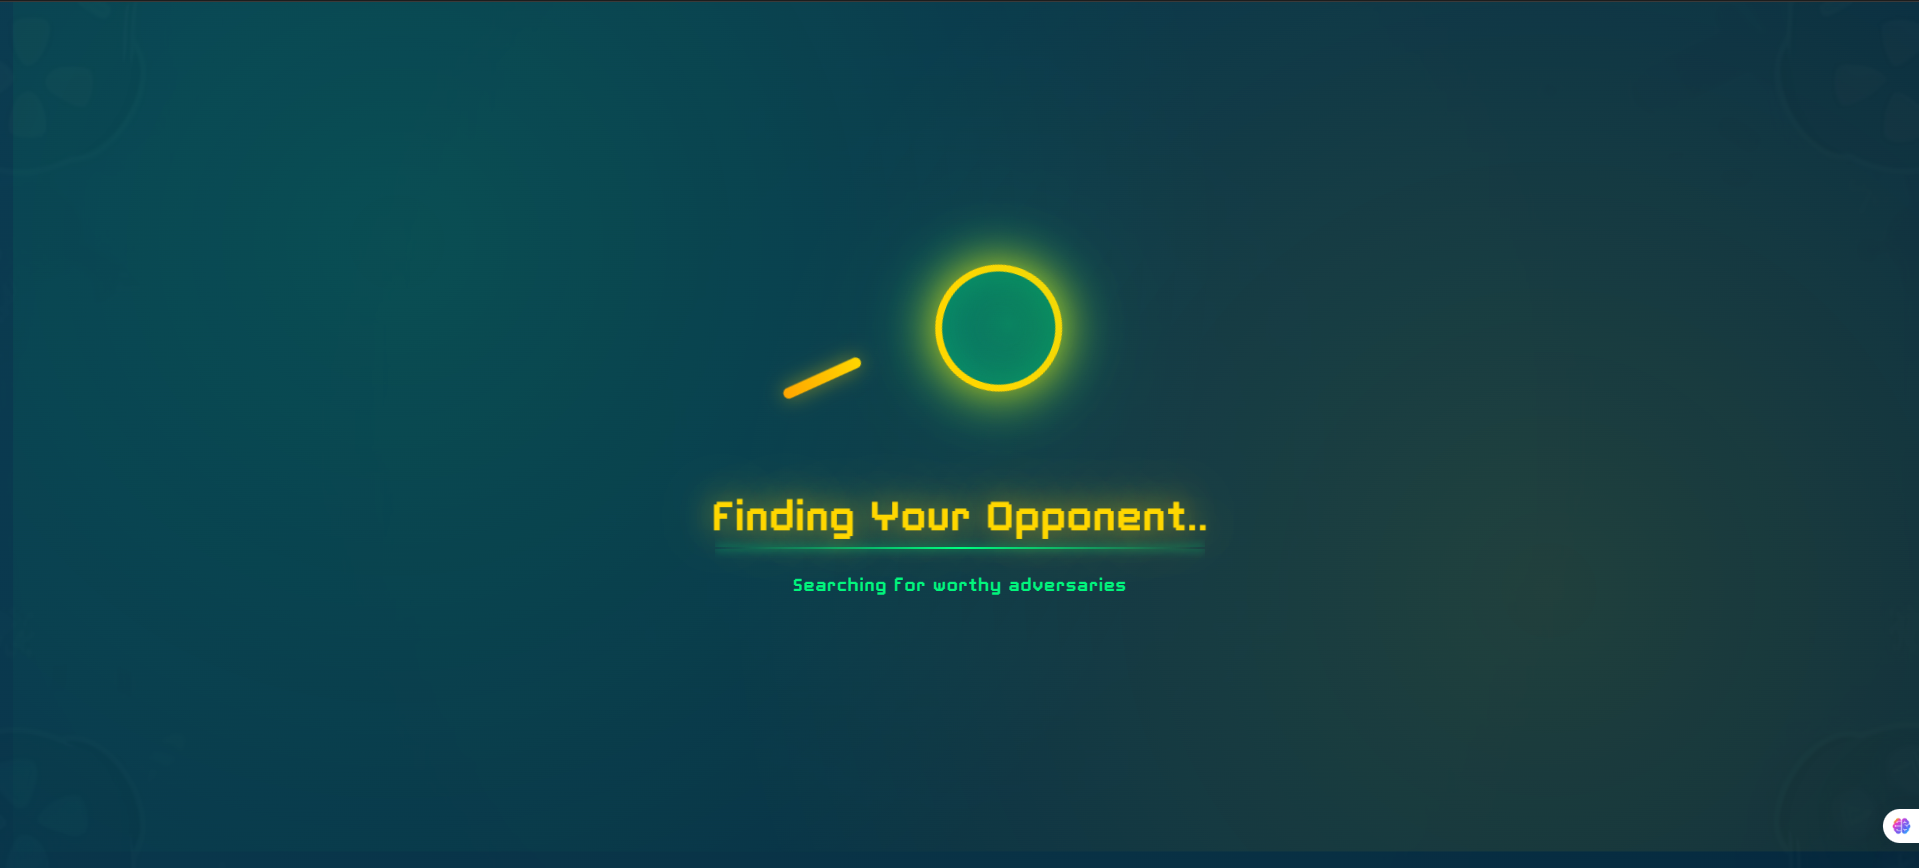
\includegraphics[width=0.9\textwidth]{loading_clan_battle.png}
\caption{Clan Battle - Matchmaking in progress}
\label{fig:clan_matchmaking}
\end{figure}

\textbf{Step 4: Opponent Clan Found - Battle Setup}
\begin{enumerate}
\item When match found, notification appears: "Opponent Clan Found!"
\item Battle details displayed:
  \begin{itemize}
    \item Opponent clan name and tag
    \item Opponent warrior list with ratings
    \item Battle format (e.g., "Best of 5 problems", "30 minutes duration")
    \item Problem difficulty range
  \end{itemize}
\item Countdown timer (5-10 seconds) before battle begins
\item All selected warriors from both clans receive notification to enter battle
\end{enumerate}

\begin{figure}[!htb]
\centering
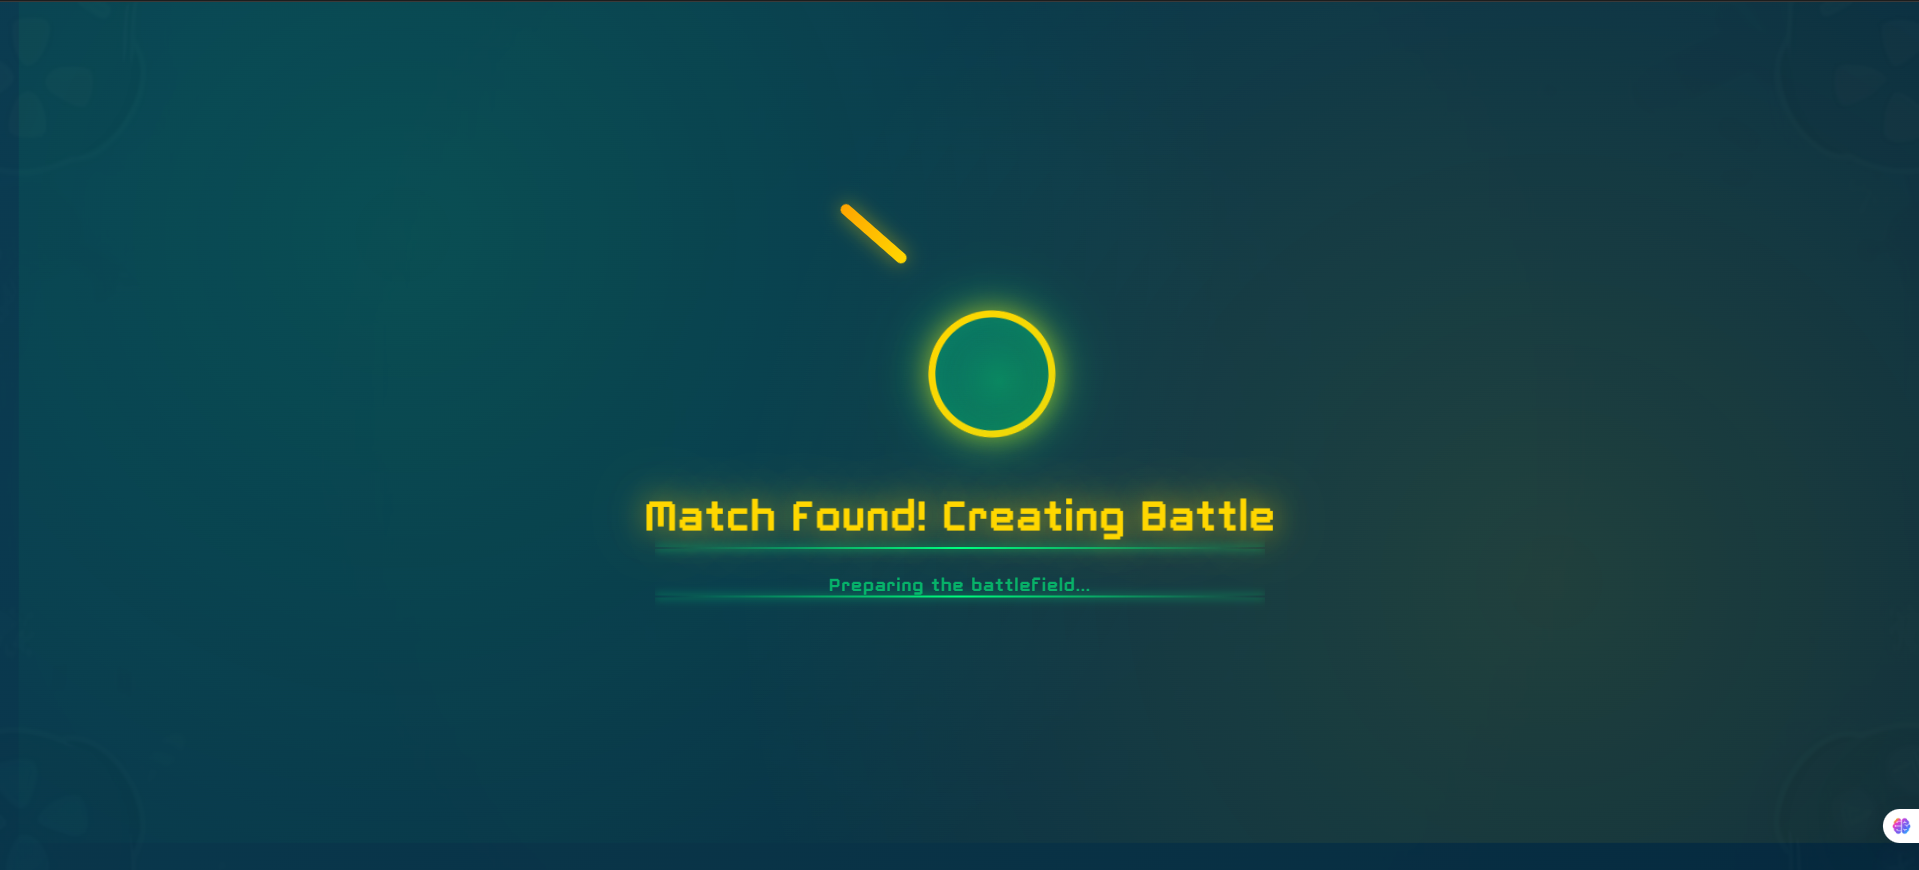
\includegraphics[width=0.9\textwidth]{clan_battle_found.png}
\caption{Clan Battle - Opponent found and battle initialization}
\label{fig:clan_opponent_found}
\end{figure}

\textbf{Step 5: Clan Battle Arena (Warrior Perspective)}

For selected warriors (regular members):

\begin{enumerate}
\item Notification received: "You have been selected for Clan Battle!"
\item Click notification or navigate to \textbf{"Clan Battle"} button
\item Battle arena loads showing:
  \begin{itemize}
    \item \textbf{Top Bar}: Your clan vs opponent clan, current score (e.g., "3-2"), battle timer
    \item \textbf{Problem Panel}: List of problems (e.g., Problem 1, Problem 2, Problem 3)
    \item \textbf{Teammate Status}: Which teammates are solving which problems
    \item \textbf{Opponent Status}: How many problems opponent clan has solved
  \end{itemize}
\item Select a problem to solve by clicking on it
\item Problem statement and code editor load (similar to PvP battle interface)
\end{enumerate}

\begin{figure}[!htb]
\centering
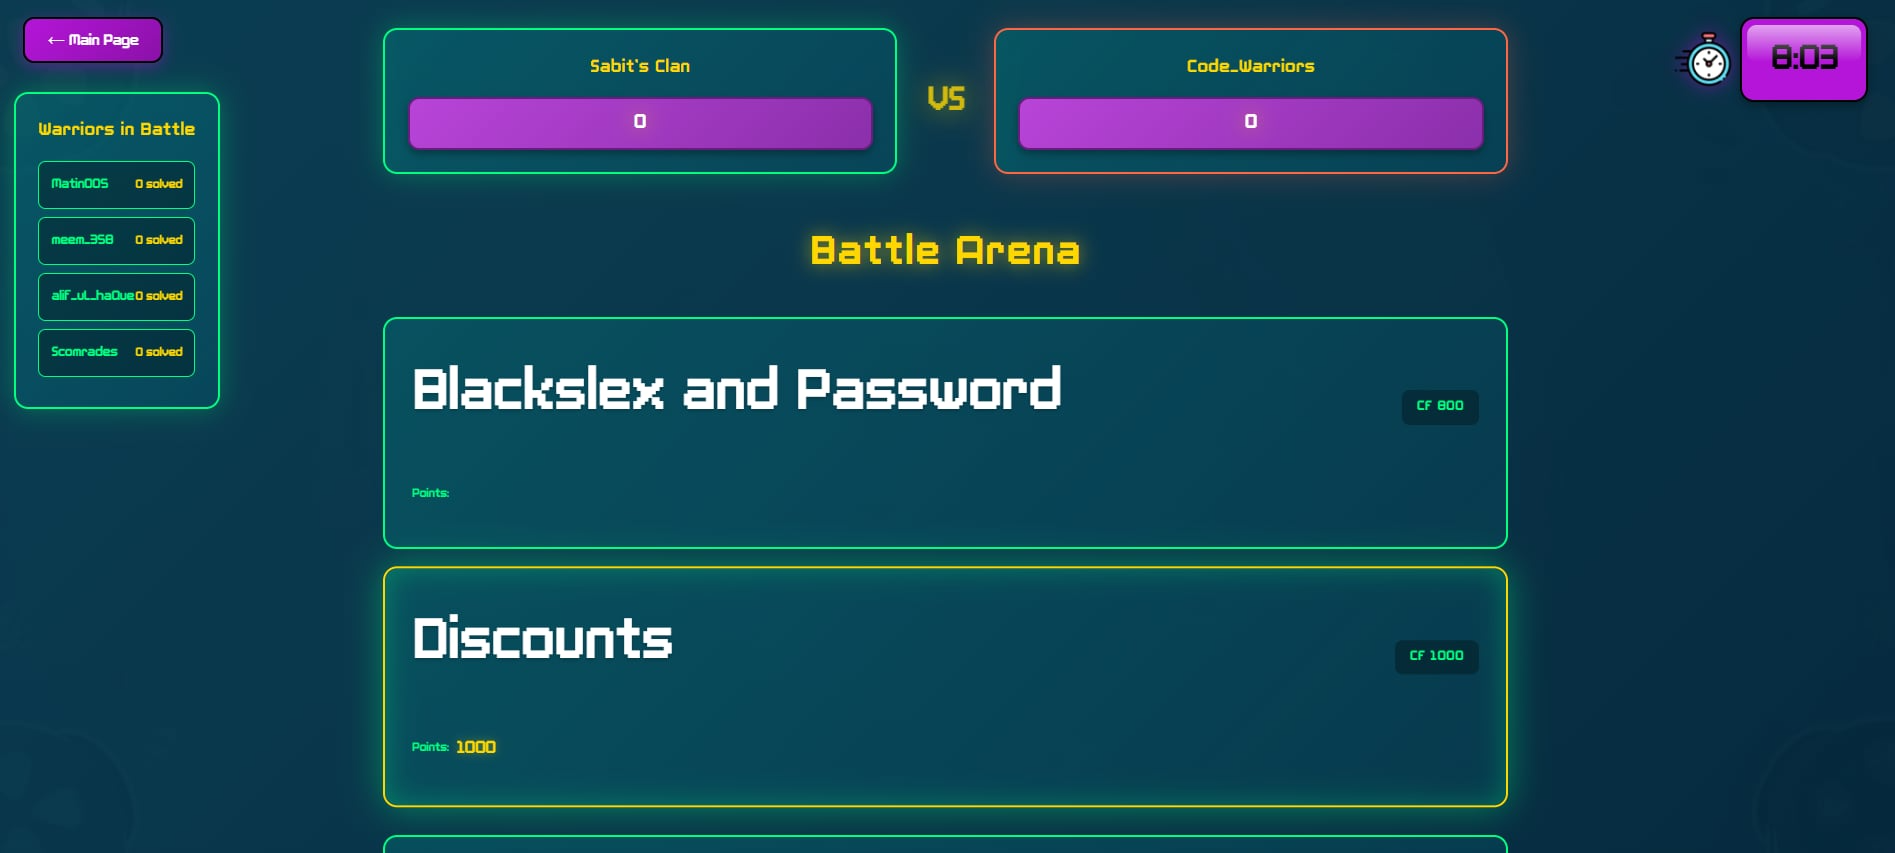
\includegraphics[width=0.9\textwidth]{clan_war_battle_arena.png}
\caption{Clan Battle Arena - Warrior view with problem selection}
\label{fig:clan_battle_arena}
\end{figure}

\textbf{Step 6: Solving Problems as Team}
\begin{enumerate}
\item Warriors can solve any available problem:
  \begin{itemize}
    \item Multiple warriors can attempt the same problem
    \item Or distribute problems strategically (coordination via clan chat)
  \end{itemize}
\item Solve problems using standard code editor:
  \begin{itemize}
    \item Write code
    \item Test locally
    \item Submit solution
  \end{itemize}
\item When any warrior gets Accepted verdict:
  \begin{itemize}
    \item Point awarded to your clan for that problem
    \item Problem marked as solved (checkmark appears)
    \item Notification sent to all clan members: "[Warrior Name] solved Problem X!"
    \item Clan score increments
  \end{itemize}
\item Continue solving remaining problems
\item Real-time score updates: "Your Clan: 4 - Opponent Clan: 3"
\end{enumerate}

\textbf{Step 7: Clan Battle Conclusion}
\begin{enumerate}
\item Battle ends when:
  \begin{itemize}
    \item Time limit reached (e.g., 30 minutes)
    \item One clan solves all problems
    \item Predetermined winning score reached
  \end{itemize}
\item Result screen displays:
  \begin{itemize}
    \item \textbf{Winner Announcement}: "Victory!" or "Defeat!"
    \item \textbf{Final Score}: Your Clan vs Opponent Clan (e.g., "5-4")
    \item \textbf{Warrior Contributions}: Which warriors solved which problems
    \item \textbf{Clan Points Earned}: Points added to clan rating
    \item \textbf{Individual XP}: Each warrior earns XP based on contribution
  \end{itemize}
\item Battle summary added to clan battle history
\item Clan leaderboards updated with new points
\item Click \textbf{"Return to Clan Page"} or \textbf{"Back to Dashboard"}
\end{enumerate}

\textbf{Non-Selected Members During Battle:}

If you are a clan member but not selected for current battle:
\begin{enumerate}
\item Clicking "Clan Battle" button shows: "No Battle Ongoing" or "Battle in progress - You are not participating"
\item You can spectate (if feature available):
  \begin{itemize}
    \item View live scores
    \item See which warriors are solving problems
    \item Cannot interact with battle
  \end{itemize}
\item Wait for next battle to potentially be selected
\end{enumerate}

\textbf{Input Requirements:}
\begin{itemize}[leftmargin=*]
\item \textbf{Leader Input}: Select 3-5 warriors from clan members, initiate matchmaking
\item \textbf{Warrior Input}: Accept battle notification, select problems to solve, submit code solutions
\item \textbf{Team Strategy}: Optional coordination via clan chat
\end{itemize}

\textbf{Output and Results:}
\begin{itemize}[leftmargin=*]
\item \textbf{Matchmaking Output}: Opponent clan found with details
\item \textbf{Battle Output}: Real-time battle arena with problems, scores, teammate status
\item \textbf{Verdicts}: Individual submission results for each warrior
\item \textbf{Battle Result}: Win/Loss/Draw, final score, clan points earned/lost, individual XP rewards
\item \textbf{Clan Statistics}: Updated clan rating, battle history, win/loss record
\end{itemize}

\textbf{Special Features:}
\begin{itemize}[leftmargin=*]
\item \textbf{Team Collaboration}: Multiple warriors working together
\item \textbf{Strategic Selection}: Leaders choose best warriors for battles
\item \textbf{Real-Time Coordination}: Live updates on teammate progress
\item \textbf{Clan Ranking}: Compete for top clan positions
\item \textbf{Collective Victory}: Team success benefits all members
\end{itemize}

\FloatBarrier

% ==================================================
\subsection{Social Features}

\subsubsection{ClashConnect - Friend and Clan Management Hub}

\textbf{Purpose:} ClashConnect serves as the central social hub for managing friend connections, viewing and responding to clan join requests (for leaders), sending battle invitations, and browsing other players' profiles.

\textbf{Step-by-Step Usage:}

\textbf{Step 1: Access ClashConnect}
\begin{enumerate}
\item From Main Dashboard, click \textbf{"ClashConnect"} button on the left navigation menu
\item If you have pending notifications (friend requests, clan join requests), a red notification badge appears on the button
\item ClashConnect interface opens showing multiple tabs or sections
\end{enumerate}

\begin{figure}[!htb]
\centering
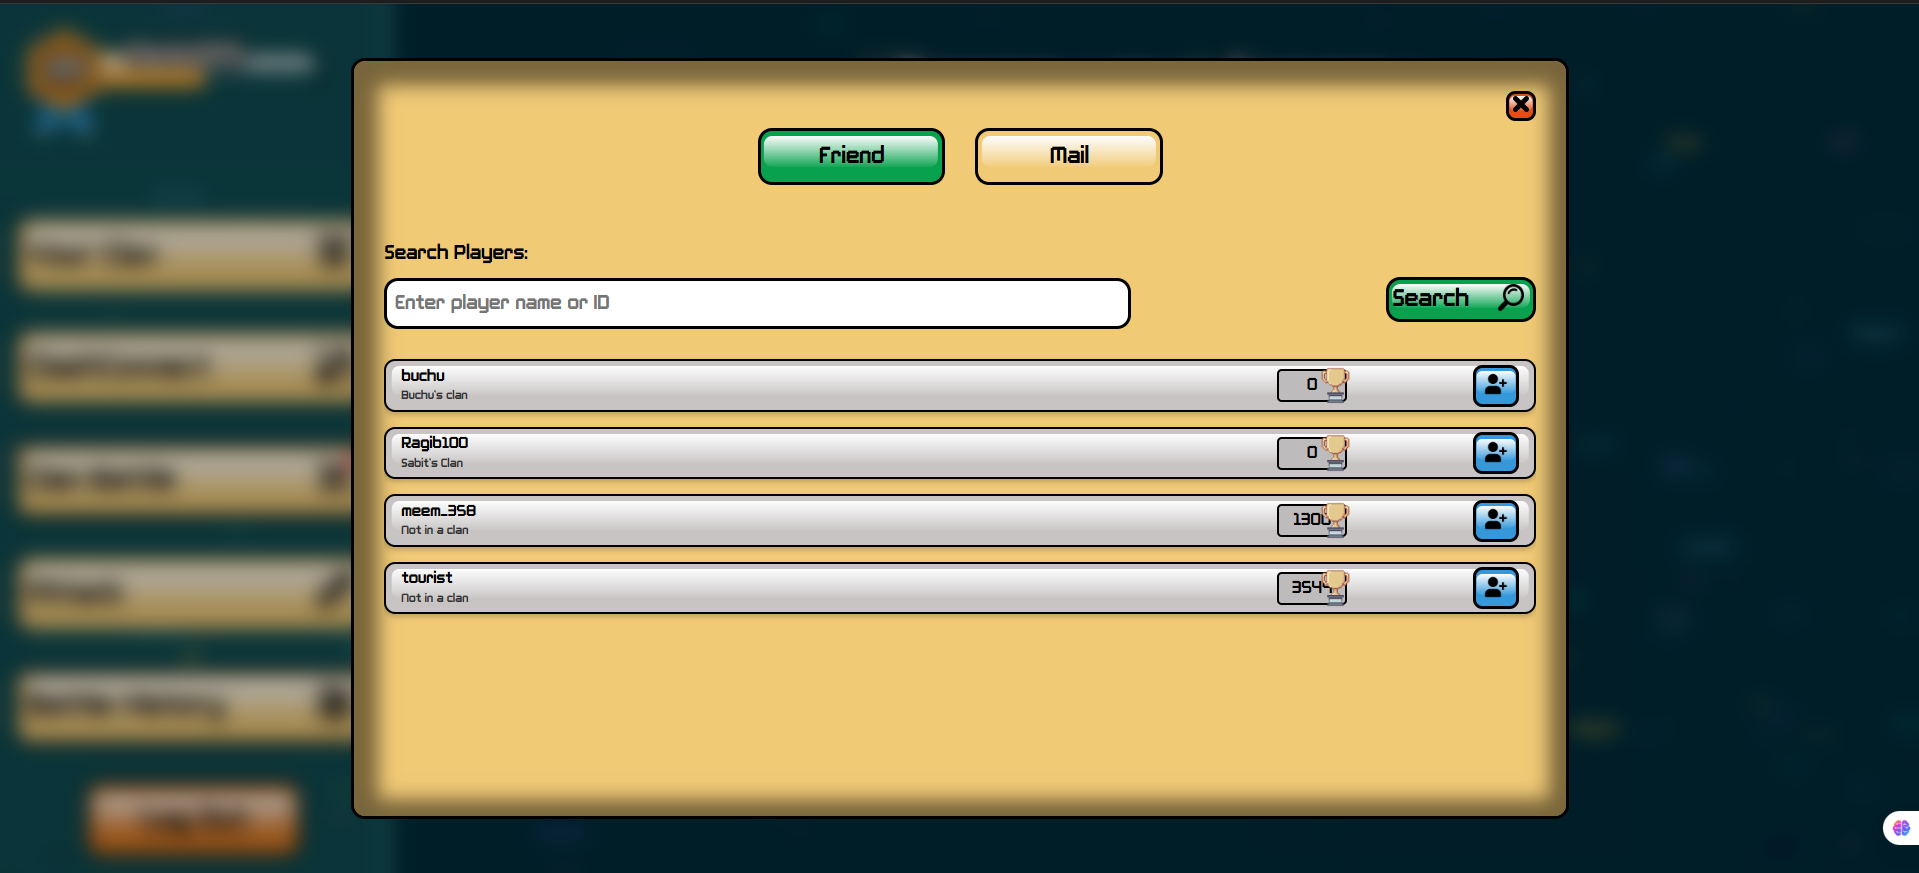
\includegraphics[width=0.9\textwidth]{clash_connect_dashboard.png}
\caption{Main Dashboard - ClashConnect access with notifications}
\label{fig:clashconnect_access}
\end{figure}

\textbf{Step 2: Browse Friend List}
\begin{enumerate}
\item ClashConnect displays your current friend list showing:
  \begin{itemize}
    \item Friend's username
    \item Current online status (green dot = online, gray = offline)
    \item Rating and level
    \item Quick action buttons: View Profile, Challenge to Battle, Remove Friend
  \end{itemize}
\item Click on a friend to view detailed profile
\item Use \textbf{"Challenge to Battle"} button to send Local Battle invitation
\end{enumerate}

\begin{figure}[!htb]
\centering
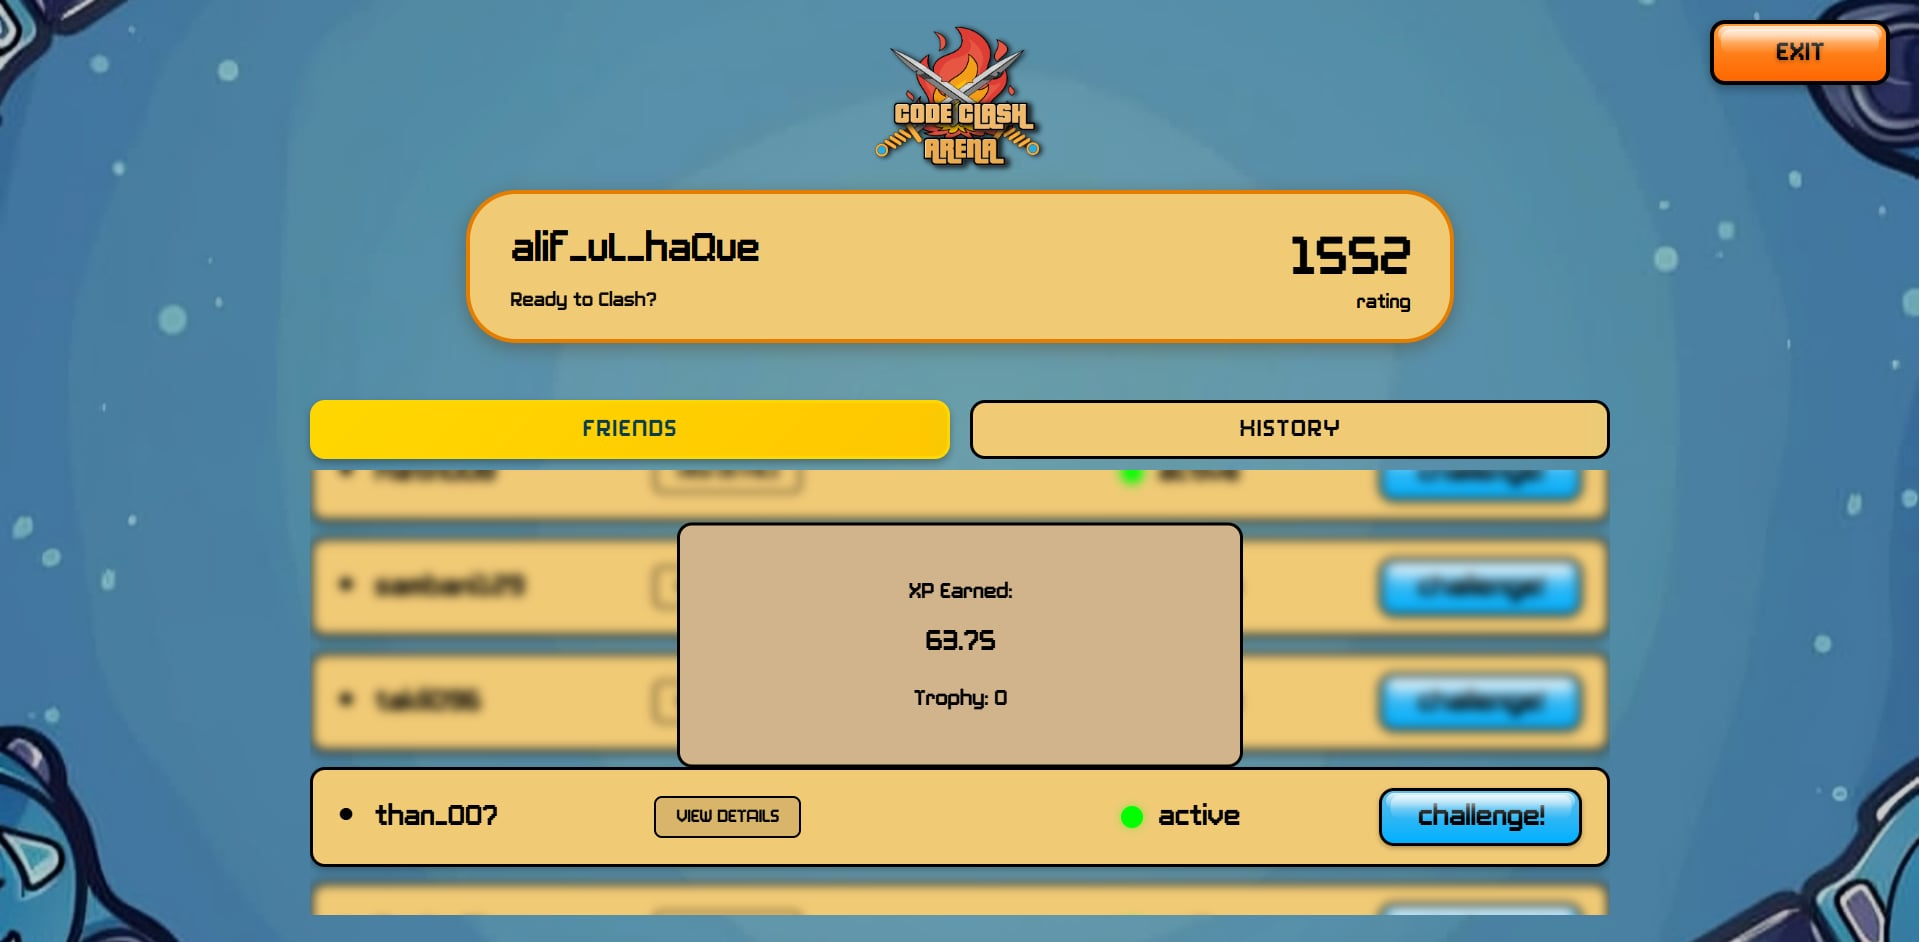
\includegraphics[width=0.9\textwidth]{local_friend.png}
\caption{ClashConnect - Friend list with online status}
\label{fig:friend_list}
\end{figure}

\textbf{Step 3: Search for New Friends}
\begin{enumerate}
\item Navigate to \textbf{"Find Friends"} or \textbf{"Search Users"} tab/section
\item Enter username in search field
\item Search results display matching users with:
  \begin{itemize}
    \item Username
    \item Rating and level
    \item Clan affiliation (if any)
    \item Current relationship status (Not Friends, Request Sent, Request Received)
  \end{itemize}
\item Click \textbf{"Add Friend"} button next to desired user
\item Confirmation: "Friend request sent to [username]"
\end{enumerate}

\textbf{Step 4: Manage Friend Requests}
\begin{enumerate}
\item Navigate to \textbf{"Pending Requests"} or \textbf{"Notifications"} section
\item View incoming friend requests showing:
  \begin{itemize}
    \item Requester's username
    \item Rating and level
    \item Time of request
  \end{itemize}
\item For each request:
  \begin{itemize}
    \item Click \textbf{"Accept"} to add as friend → Success: "[Username] is now your friend"
    \item Click \textbf{"Reject"} to decline → Request removed
    \item Click username to view full profile before deciding
  \end{itemize}
\item Accepted friends immediately appear in your friend list
\end{enumerate}

\begin{figure}[!htb]
\centering
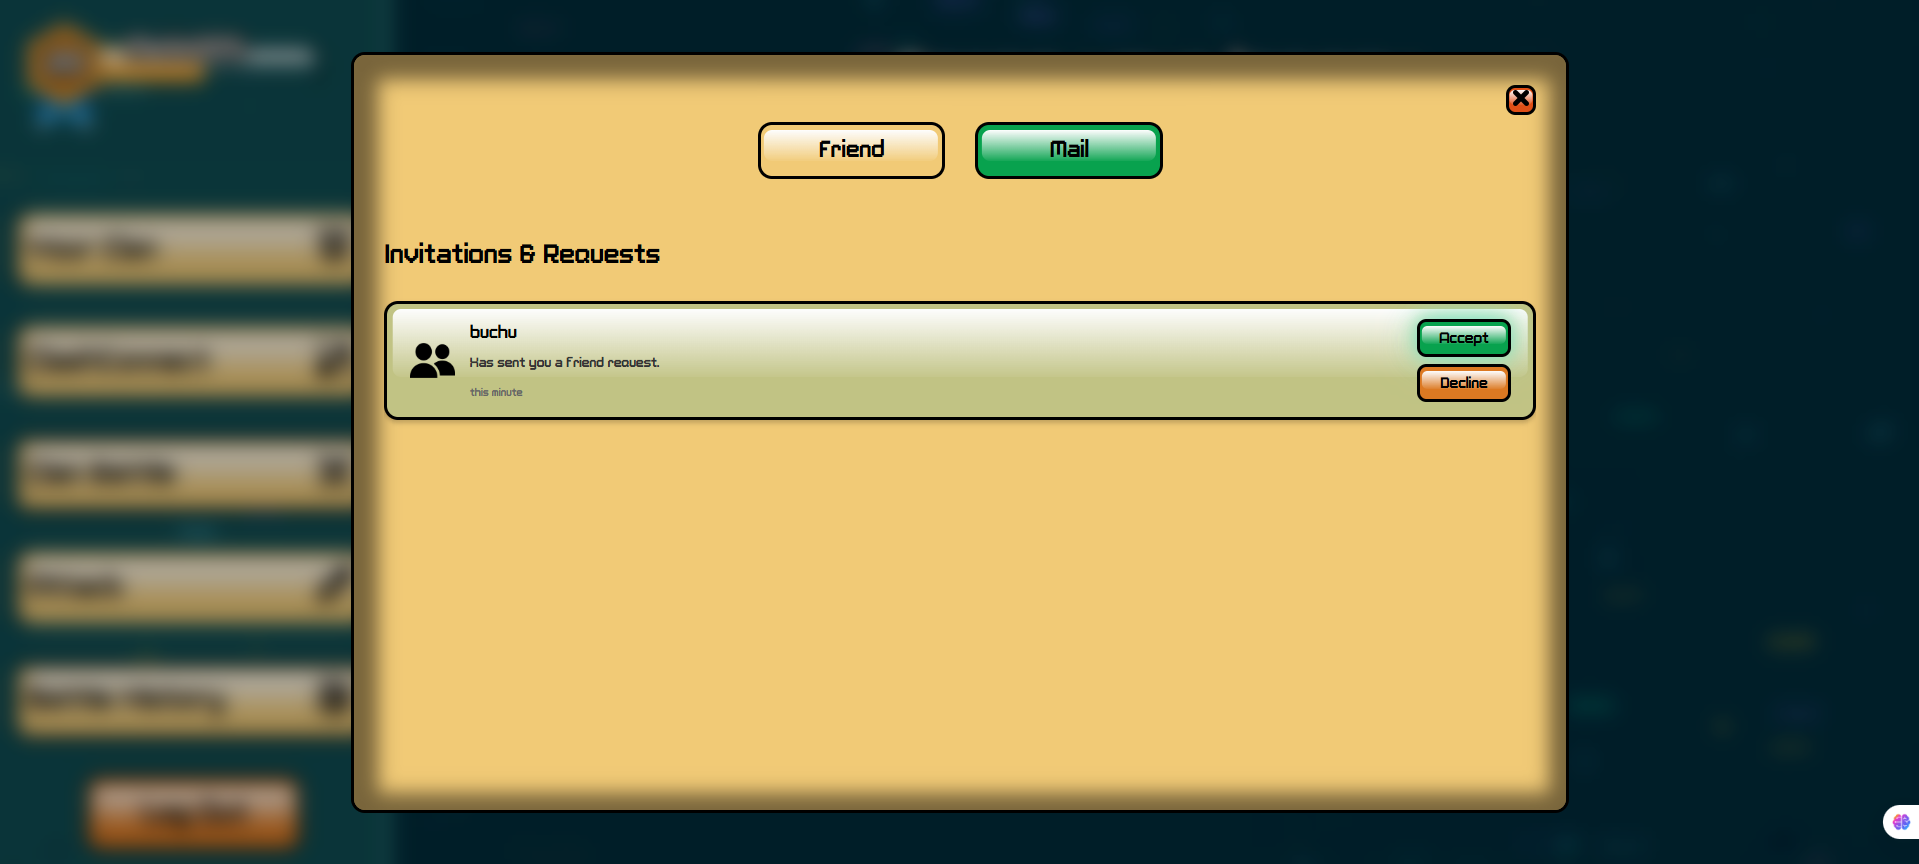
\includegraphics[width=0.9\textwidth]{manage_clash_connect.png}
\caption{ClashConnect - Managing incoming friend requests}
\label{fig:friend_requests}
\end{figure}

\textbf{Step 5: Clan Join Requests (Clan Leaders Only)}

If you are a clan leader, ClashConnect also displays clan join requests:

\begin{enumerate}
\item Navigate to \textbf{"Clan Requests"} tab (only visible to leaders)
\item View users who requested to join your clan:
  \begin{itemize}
    \item Applicant username
    \item Rating and level
    \item Current clan status (not in clan / left previous clan)
    \item Application time
  \end{itemize}
\item Click on applicant to view detailed profile and statistics
\item Decision options:
  \begin{itemize}
    \item \textbf{"Accept"}: User joins your clan immediately, receives notification
    \item \textbf{"Reject"}: Request denied, user can apply again or join other clans
  \end{itemize}
\item Clan member list updates automatically when requests are accepted
\end{enumerate}

\begin{figure}[!htb]
\centering
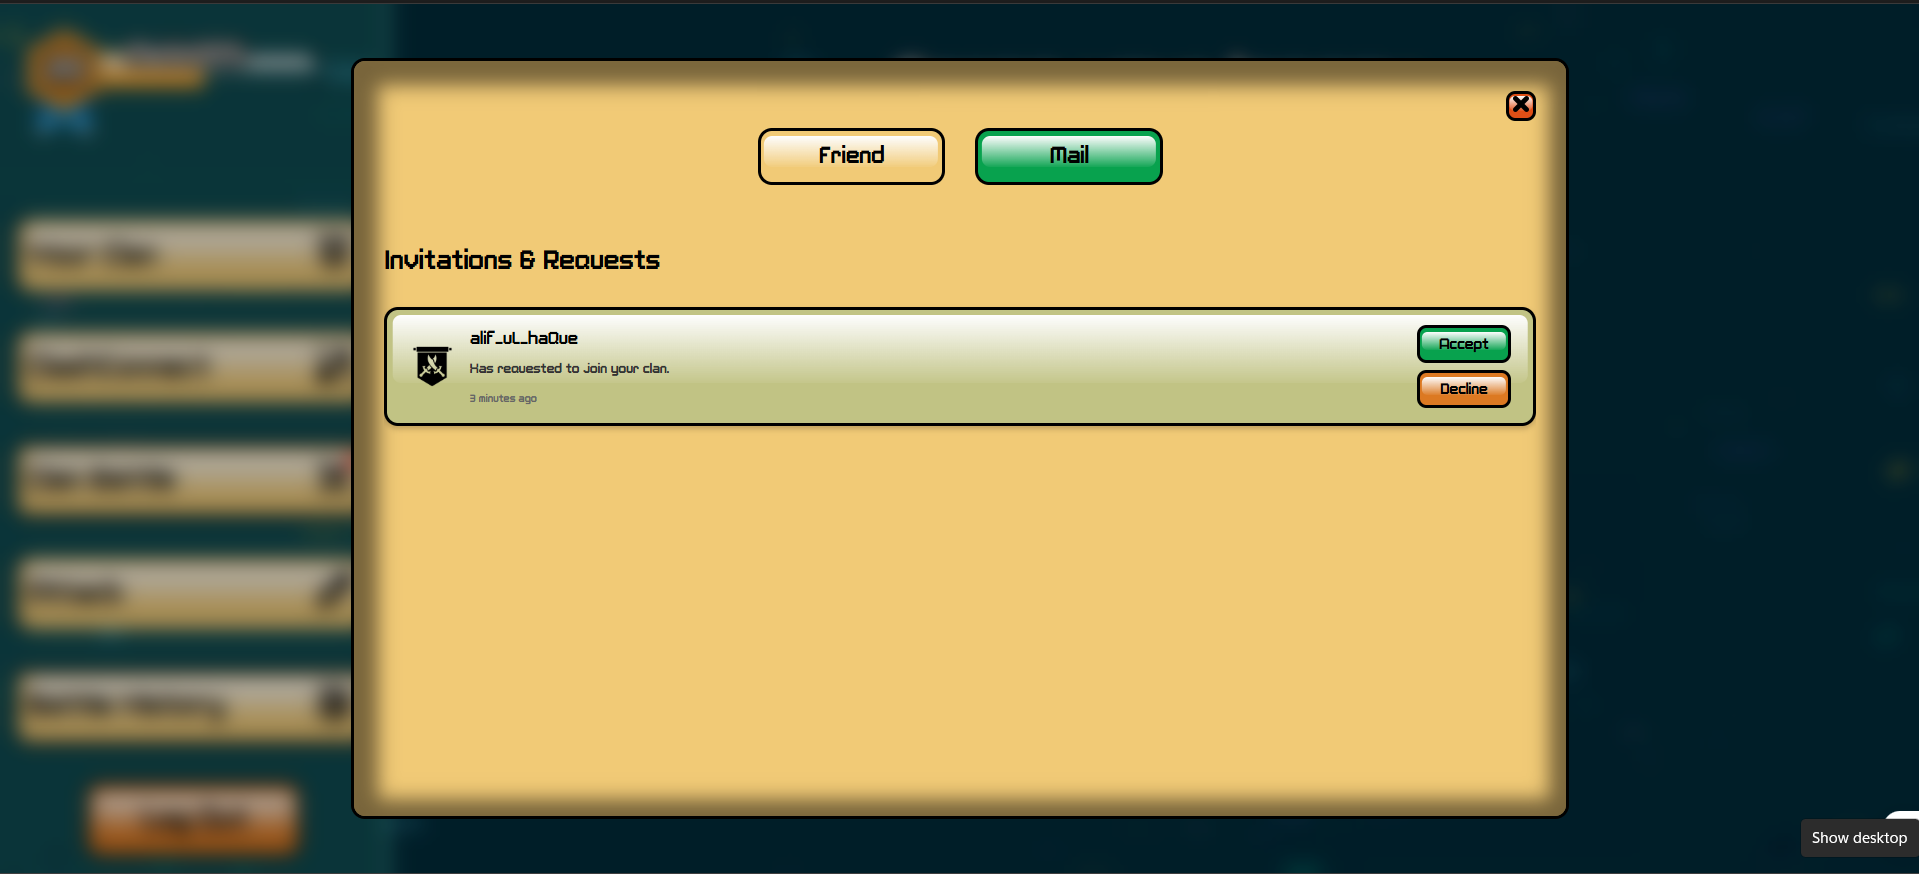
\includegraphics[width=0.9\textwidth]{incoming_clan_join_request.png}
\caption{ClashConnect - Clan join requests (leader view)}
\label{fig:clan_requests_leader}
\end{figure}

\textbf{Step 6: View Player Profiles}
\begin{enumerate}
\item Click on any username (from friend list, search results, or leaderboards)
\item Player profile page displays:
  \begin{itemize}
    \item Username and avatar
    \item Rating, level, and XP progress
    \item Clan affiliation and tag
    \item Battle statistics: Win/Loss record, total battles, win rate percentage
    \item Recent battle history
    \item Problems solved count
    \item Join date
  \end{itemize}
\item Action buttons available:
  \begin{itemize}
    \item \textbf{"Add Friend"} (if not friends)
    \item \textbf{"Challenge to Battle"} (if friends or available)
    \item \textbf{"View Clan"} (if player is in a clan)
    \item \textbf{"Remove Friend"} (if already friends)
  \end{itemize}
\item Click \textbf{"Back"} to return to ClashConnect
\end{enumerate}

\textbf{Input Requirements:}
\begin{itemize}[leftmargin=*]
\item \textbf{Friend Search}: Username or partial username
\item \textbf{Friend Request}: Target user must exist and not already be friend
\item \textbf{Clan Request Management (Leaders)}: Decision to accept or reject applicants
\end{itemize}

\textbf{Output and Results:}
\begin{itemize}[leftmargin=*]
\item \textbf{Friend List Output}: Display of all friends with online status
\item \textbf{Search Output}: List of users matching search query
\item \textbf{Request Output}: Notifications for pending friend/clan requests
\item \textbf{Profile Output}: Detailed player information and statistics
\item \textbf{Relationship Updates}: Friend added/removed confirmations
\end{itemize}

\textbf{Special Features:}
\begin{itemize}[leftmargin=*]
\item \textbf{Centralized Hub}: All social features in one interface
\item \textbf{Real-Time Notifications}: Instant updates for new requests
\item \textbf{Online Status}: See which friends are currently active
\item \textbf{Quick Challenges}: Send battle invitations directly from friend list
\item \textbf{Clan Management Integration}: Leaders manage both friends and clan members
\end{itemize}

\FloatBarrier

% ==================================================
% SECTION 6: NAVIGATION GUIDE
% ==================================================

\section{Navigation Guide}

This section provides a comprehensive guide to navigating CodeClash Arena's interface. After logging in, you will be directed to the Main Dashboard, which serves as the central hub for accessing all platform features.

\subsection{Main Dashboard Overview}

The Main Dashboard features an animated background with coding-themed particles and a vertical menu bar on the left side. At the top of the menu, you will see your XP bar displaying your current level, experience points, and username. Below the XP bar are five main navigation buttons and a logout option.

\subsection{Navigation Options}

\subsubsection{Your Clan}

Access your clan management interface and view clan details. If you are not currently in a clan, clicking this button opens the clan browsing menu where you can search for clans to join or create your own clan. If you are already a clan member, this opens your clan's information page showing member list, clan statistics, total points, and war history.

\subsubsection{ClashConnect}

Open the social hub to manage your connections and invitations. This feature allows you to search for other players, send and accept friend requests, view incoming clan join requests (if you are a clan leader), and manage your friend list. A notification badge appears on this button when you have pending friend requests or clan join requests.

\subsubsection{Clan Battle}

Navigate to the clan battle interface for team-based competitions. If you are a clan leader, clicking this button takes you to the team selection page where you can choose warriors and initiate matchmaking for clan battles. If you are a regular clan member and a battle is ongoing, you will be directed to the battle arena; otherwise, you will see a "No Battle Ongoing" message. A notification badge appears when there is an active clan battle.

\subsubsection{Attack}

Launch the PvP battle menu to compete in 1v1 coding challenges. This button opens an overlay menu with multiple battle mode options: Global Battle Mode (matchmaking with players of similar rating), Local Battle Mode (challenge specific friends), and Practice Gym (solo practice without competition). Select your preferred mode to begin competitive coding.

\subsubsection{Battle History}

View your complete battle record and performance statistics. This section displays all your past 1v1 battles and clan battles, showing opponents faced, problems solved, battle outcomes (win/loss), time taken, and rating changes. Use this feature to analyze your performance trends and track your improvement over time.

\subsubsection{Log Out}

Securely end your current session and return to the homepage. Clicking this button clears your authentication tokens and logs you out of the platform. Always use this option when accessing CodeClash Arena from shared or public computers to protect your account security.

\FloatBarrier

% ==================================================
% SECTION 7: ERROR HANDLING AND MESSAGES
% ==================================================

\section{Error Handling and Messages}

CodeClash Arena displays color-coded alerts to communicate system status: green alerts for successful actions (e.g., "Sign in successful!") and red alerts for errors. Alerts disappear automatically after a few seconds or can be manually closed.

\subsection{Authentication Errors}

\textbf{Invalid Login Credentials}

\textit{Error Message:} "Invalid login credentials" or "Invalid email or password"

\textit{Solutions:} Verify email and password are correct; check Caps Lock is off; ensure no extra spaces; use correct email (not Codeforces handle); verify email has been confirmed after signup.

\textbf{Email Not Confirmed/Verified}

\textit{Error Message:} "Email not confirmed" or "Error fetching user data"

\textit{Solutions:} Check inbox and spam folder for verification email from Supabase; look for subject "Confirm Your Email"; click verification link; return to log in page after verification; contact support if link expired (24 hours).

\textbf{Account Locked}

\textit{Error Message:} "Too many login attempts"

\textit{Solutions:} Wait 15-30 minutes before retrying; use password reset if needed; avoid multiple attempts during lockout.

\textbf{Input Requirements:}
\begin{itemize}[leftmargin=*]
\item \textbf{No Direct Input}: Leaderboards are view-only, automatically populated
\item \textbf{Optional Filters}: Select time period or category for custom rankings
\end{itemize}

\textbf{Output and Results:}
\begin{itemize}[leftmargin=*]
\item \textbf{Player Rankings}: Sorted list of players by rating, XP, or other criteria
\item \textbf{Clan Rankings}: Sorted list of clans by points and performance
\item \textbf{Your Position}: Highlighted rank showing your standing
\item \textbf{Statistics}: Win rates, battle counts, and performance metrics
\item \textbf{Real-Time Updates}: Rankings update after each battle completion
\end{itemize}

\textbf{Special Features:}
\begin{itemize}[leftmargin=*]
\item \textbf{Live Rankings}: Real-time updates as battles conclude
\item \textbf{Multiple Categories}: Different ranking criteria available
\item \textbf{Top Player Recognition}: Special badges for top 3 positions
\item \textbf{Personal Tracking}: Easy identification of your own rank
\item \textbf{Competitive Motivation}: Track progress toward top positions
\end{itemize}

\FloatBarrier

% ==================================================
\subsection{Profile and Statistics}

\textbf{Purpose:} View and manage your personal profile, track your coding progress, monitor statistics, and update account settings including Codeforces handle.

\textbf{Step-by-Step Usage:}

\textbf{Step 1: Access Your Profile}
\begin{enumerate}
\item From Main Dashboard, click on your \textbf{username} or \textbf{profile icon} (typically in top-right corner or navigation menu)
\item Dropdown menu appears with options including \textbf{"View Profile"} or \textbf{"My Profile"}
\item Click \textbf{"View Profile"}
\item Your profile page loads
\end{enumerate}

\begin{figure}[!htb]
\centering
\fbox{\parbox{0.9\textwidth}{\centering\vspace{3cm}[Screenshot: User menu dropdown with "View Profile" option highlighted]\vspace{3cm}}}
\caption{Access Profile from user menu}
\label{fig:profile_access}
\end{figure}

\textbf{Step 2: Profile Overview}

Your profile displays comprehensive information:

\begin{itemize}[leftmargin=*]
\item \textbf{Personal Information}:
  \begin{itemize}
    \item Username
    \item Avatar/profile picture (if available)
    \item Join date
    \item Email address (partially hidden for privacy)
    \item Linked Codeforces handle
  \end{itemize}
\item \textbf{Progression Statistics}:
  \begin{itemize}
    \item Current Level (e.g., Level 15)
    \item XP Bar showing progress to next level (e.g., "2,450 / 3,000 XP")
    \item Total XP earned
  \end{itemize}
\item \textbf{Rating and Ranking}:
  \begin{itemize}
    \item Current ELO rating (e.g., 1,580)
    \item Global rank (e.g., "\#247 Globally")
    \item Rating progress graph (optional visual chart)
  \end{itemize}
\item \textbf{Battle Statistics}:
  \begin{itemize}
    \item Total battles fought
    \item Wins / Losses / Draws
    \item Win rate percentage (e.g., "65\% win rate")
    \item Average battle time
  \end{itemize}
\item \textbf{Problem Solving Stats}:
  \begin{itemize}
    \item Total problems solved
    \item Problems by difficulty (Easy: X, Medium: Y, Hard: Z)
    \item Favorite problem tags
  \end{itemize}
\item \textbf{Clan Information}:
  \begin{itemize}
    \item Current clan name and tag (if in a clan)
    \item Role in clan (Leader / Member)
    \item Clan contribution points
  \end{itemize}
\end{itemize}

\begin{figure}[!htb]
\centering
\fbox{\parbox{0.9\textwidth}{\centering\vspace{3cm}[Screenshot: Complete profile page showing all statistics sections (personal info, rating, battles, problems, clan)]\vspace{3cm}}}
\caption{User Profile - Complete statistics overview}
\label{fig:profile_overview}
\end{figure}

\textbf{Step 3: View Battle History}
\begin{enumerate}
\item Scroll down to \textbf{"Recent Battles"} section in profile
\item Or click \textbf{"View Full Battle History"} button
\item Battle history displays list of past battles:
  \begin{itemize}
    \item Date and time of battle
    \item Battle type (Global / Local / Clan)
    \item Opponent username (or clan name for clan battles)
    \item Problem solved (with link to Codeforces problem)
    \item Result (Win / Loss / Draw)
    \item Rating change (e.g., "+12", "-8")
    \item Time taken
  \end{itemize}
\item Click on individual battle to see detailed battle summary
\item Pagination available for viewing older battles
\end{enumerate}

\begin{figure}[!htb]
\centering
\fbox{\parbox{0.9\textwidth}{\centering\vspace{3cm}[Screenshot: Battle history section showing list of past battles with results and rating changes]\vspace{3cm}}}
\caption{Battle History - Record of all past battles}
\label{fig:battle_history_profile}
\end{figure}

\textbf{Step 4: Edit Profile Settings}
\begin{enumerate}
\item Click \textbf{"Edit Profile"} or \textbf{"Settings"} button
\item Profile settings page opens with editable fields:
  \begin{itemize}
    \item \textbf{Codeforces Handle}: Update linked Codeforces username
      \begin{itemize}
        \item Enter new handle
        \item System validates handle exists on Codeforces
        \item Note: Handle changes may be rate-limited (e.g., once per month)
      \end{itemize}
    \item \textbf{Avatar}: Upload profile picture (if feature available)
    \item \textbf{Bio}: Add personal description (optional)
    \item \textbf{Notification Preferences}: Enable/disable email notifications for:
      \begin{itemize}
        \item Friend requests
        \item Battle invitations
        \item Clan announcements
      \end{itemize}
    \item \textbf{Privacy Settings}: Control who can:
      \begin{itemize}
        \item Send you friend requests
        \item Challenge you to battles
        \item View your battle history
      \end{itemize}
  \end{itemize}
\item Make desired changes
\item Click \textbf{"Save Changes"} button
\item Success notification: "Profile updated successfully"
\end{enumerate}

\begin{figure}[!htb]
\centering
\fbox{\parbox{0.9\textwidth}{\centering\vspace{3cm}[Screenshot: Profile settings page with Codeforces handle field, notification toggles, and Save button highlighted]\vspace{3cm}}}
\caption{Profile Settings - Edit personal information and preferences}
\label{fig:profile_settings}
\end{figure}

\textbf{Step 5: View Progress Graphs (Optional)}

If analytics are available:
\begin{enumerate}
\item Navigate to \textbf{"Statistics"} or \textbf{"Analytics"} tab in profile
\item View visual representations:
  \begin{itemize}
    \item \textbf{Rating Progress Graph}: Line chart showing rating changes over time
    \item \textbf{Battle Activity}: Calendar heatmap or bar chart of battles per day/week
    \item \textbf{Problem Difficulty Distribution}: Pie chart of solved problems by difficulty
    \item \textbf{Win Rate Trend}: Graph showing win rate over time
  \end{itemize}
\item Hover over graph elements for detailed tooltips
\item Use date range selector to filter time periods
\end{enumerate}

\begin{figure}[!htb]
\centering
\fbox{\parbox{0.9\textwidth}{\centering\vspace{3cm}[Screenshot: Statistics page with rating graph and problem distribution charts]\vspace{3cm}}}
\caption{Profile Statistics - Visual analytics and progress tracking}
\label{fig:profile_analytics}
\end{figure}

\textbf{Input Requirements:}
\begin{itemize}[leftmargin=*]
\item \textbf{Profile Access}: No input required (automatic based on logged-in user)
\item \textbf{Settings Update}: New Codeforces handle (must be valid), avatar image (if uploading), preference selections
\end{itemize}

\textbf{Output and Results:}
\begin{itemize}[leftmargin=*]
\item \textbf{Profile Display}: Complete statistics, ratings, battle history
\item \textbf{Progress Tracking}: XP bar, level, rating changes
\item \textbf{Battle Record}: Detailed history of all battles
\item \textbf{Settings Confirmation}: Success messages for updates
\item \textbf{Analytics}: Visual graphs of progress (if available)
\end{itemize}

\textbf{Special Features:}
\begin{itemize}[leftmargin=*]
\item \textbf{Comprehensive Stats}: All-in-one view of your coding journey
\item \textbf{Progress Tracking}: Visual XP bar and level progression
\item \textbf{Rating History}: Track rating changes after each battle
\item \textbf{Codeforces Integration}: Update linked handle for submissions
\item \textbf{Privacy Controls}: Manage who can interact with you
\end{itemize}

\FloatBarrier

% ==================================================
\subsection{Code Editor Features}

\textbf{Purpose:} The integrated code editor provides a comprehensive coding environment within the browser, supporting multiple programming languages, syntax highlighting, local testing, and seamless submission to Codeforces judge.

\textbf{Key Features Overview:}

The code editor is accessible in all coding contexts (Global Battles, Local Battles, Clan Battles, Practice Gym) and provides consistent functionality across all modes.

\textbf{Step-by-Step Usage:}

\textbf{Step 1: Editor Interface}

When entering any battle or practice session, the code editor appears with:

\begin{itemize}[leftmargin=*]
\item \textbf{Editing Area}:
  \begin{itemize}
    \item Large text area for writing code
    \item Line numbers displayed on left margin
    \item Syntax highlighting based on selected language
    \item Auto-indentation support
    \item Code folding for functions/blocks (if available)
  \end{itemize}
\item \textbf{Top Toolbar}:
  \begin{itemize}
    \item Language selector dropdown
    \item Font size adjustment (if available)
    \item Theme toggle (light/dark mode, if available)
  \end{itemize}
\item \textbf{Bottom Action Bar}:
  \begin{itemize}
    \item \textbf{"Run Code"} button (local testing)
    \item \textbf{"Submit"} button (official submission)
    \item \textbf{"Reset"} button (clear code)
  \end{itemize}
\end{itemize}

\begin{figure}[!htb]
\centering
\fbox{\parbox{0.9\textwidth}{\centering\vspace{3cm}[Screenshot: Code editor interface showing editing area, language dropdown, line numbers, and action buttons]\vspace{3cm}}}
\caption{Code Editor - Main interface components}
\label{fig:code_editor_interface}
\end{figure}

\textbf{Step 2: Select Programming Language}
\begin{enumerate}
\item Click on the \textbf{language dropdown menu} (typically shows default like "C++")
\item Available languages include:
  \begin{itemize}
    \item C++ (multiple versions: C++11, C++14, C++17, C++20)
    \item Java (Java 8, Java 11, Java 17)
    \item Python (Python 2, Python 3)
    \item JavaScript (Node.js)
    \item C (C99, C11)
    \item Others: Go, Rust, Kotlin (depending on Codeforces support)
  \end{itemize}
\item Select your preferred language
\item Editor syntax highlighting automatically updates to match selected language
\item Template code may auto-populate (e.g., \texttt{int main()} for C++, \texttt{public class Main} for Java)
\end{enumerate}

\begin{figure}[!htb]
\centering
\fbox{\parbox{0.9\textwidth}{\centering\vspace{3cm}[Screenshot: Language dropdown expanded showing list of available programming languages]\vspace{3cm}}}
\caption{Language Selection - Choose programming language}
\label{fig:language_selection}
\end{figure}

\textbf{Step 3: Write Code}
\begin{enumerate}
\item Click in the editing area and start typing your solution
\item Editor features while typing:
  \begin{itemize}
    \item \textbf{Syntax Highlighting}: Keywords, strings, comments colored for readability
    \item \textbf{Auto-Indentation}: Automatic indentation when pressing Enter
    \item \textbf{Bracket Matching}: Matching brackets highlighted when cursor adjacent
    \item \textbf{Tab Support}: Tab key inserts spaces (typically 2 or 4 spaces)
    \item \textbf{Undo/Redo}: Ctrl+Z / Ctrl+Y for undo and redo
    \item \textbf{Copy/Paste}: Standard clipboard operations (Ctrl+C, Ctrl+V)
    \item \textbf{Find/Replace}: Ctrl+F to search within code (if available)
  \end{itemize}
\item Write your complete solution
\item Use line numbers for reference and debugging
\end{enumerate}

\begin{figure}[!htb]
\centering
\fbox{\parbox{0.9\textwidth}{\centering\vspace{3cm}[Screenshot: Code editor with sample code written, showing syntax highlighting and line numbers]\vspace{3cm}}}
\caption{Code Editor - Writing code with syntax highlighting}
\label{fig:code_writing}
\end{figure}

\textbf{Step 4: Local Testing with Piston API}
\begin{enumerate}
\item After writing code, click \textbf{"Run Code"} or \textbf{"Test"} button
\item Test input panel appears:
  \begin{itemize}
    \item \textbf{Input Field}: Text area to enter test input data
    \item Sample test cases from problem may be pre-filled
    \item You can modify or enter custom test cases
  \end{itemize}
\item Enter input data matching problem's input format
\item Click \textbf{"Run"} or \textbf{"Execute"} button
\item Code executes locally using Piston API (remote code execution service)
\item Wait for execution (typically 1-3 seconds)
\item Test results display:
  \begin{itemize}
    \item \textbf{Your Output}: What your code produced
    \item \textbf{Expected Output}: Sample output from problem (if available)
    \item \textbf{Execution Time}: Time taken in milliseconds
    \item \textbf{Memory Used}: Memory consumption (if available)
    \item \textbf{Status}: Success (ran without errors) or Error (runtime/compilation error)
  \end{itemize}
\item If compilation error or runtime error:
  \begin{itemize}
    \item Error message displays with details
    \item Line number of error (if available)
    \item Fix code and test again
  \end{itemize}
\item Run multiple test cases to verify correctness
\end{enumerate}

\begin{figure}[!htb]
\centering
\fbox{\parbox{0.9\textwidth}{\centering\vspace{3cm}[Screenshot: Test panel showing input field, Run button, and output results comparing expected vs actual output]\vspace{3cm}}}
\caption{Local Testing - Test code with custom inputs}
\label{fig:local_testing_detailed}
\end{figure}

\textbf{Step 5: Submit to Codeforces Judge}
\begin{enumerate}
\item Once confident code is correct, click \textbf{"Submit"} button
\item Confirmation dialog may appear: "Submit code to Codeforces judge?"
\item Click \textbf{"Confirm"}
\item Submission process begins:
  \begin{itemize}
    \item Code sent to Codeforces servers
    \item Your linked Codeforces handle used for submission
    \item Selected language and problem ID included in submission
  \end{itemize}
\item Submission status updates in real-time:
  \begin{itemize}
    \item "Submitting..." (sending code to Codeforces)
    \item "In Queue" (waiting for judge)
    \item "Running on test 1", "Running on test 2", ... (executing against test cases)
  \end{itemize}
\item Final verdict appears (typically within 5-15 seconds):
  \begin{itemize}
    \item \textbf{Accepted (AC)}: All test cases passed \checkmark{} (green color)
    \item \textbf{Wrong Answer (WA)}: Failed on test case X (red color)
    \item \textbf{Time Limit Exceeded (TLE)}: Code too slow on test X (yellow/orange)
    \item \textbf{Runtime Error (RE)}: Code crashed on test X (red color)
    \item \textbf{Memory Limit Exceeded (MLE)}: Used too much memory
    \item \textbf{Compilation Error (CE)}: Code doesn't compile
  \end{itemize}
\item Detailed verdict information shown:
  \begin{itemize}
    \item Test case number where error occurred (if failed)
    \item Execution time for each test (if available)
    \item Verdict message from Codeforces
  \end{itemize}
\end{enumerate}

\begin{figure}[!htb]
\centering
\fbox{\parbox{0.9\textwidth}{\centering\vspace{3cm}[Screenshot: Submission in progress showing "Running on test 5" status with progress indicator]\vspace{3cm}}}
\caption{Code Submission - Real-time verdict tracking}
\label{fig:submission_progress}
\end{figure}

\textbf{Step 6: Handle Verdicts}

\textbf{If Accepted:}
\begin{itemize}[leftmargin=*]
\item Success notification displays
\item In battles: You win the battle (or contribute point to clan)
\item In practice: Problem marked as solved, XP awarded
\item Option to view full submission details on Codeforces
\end{itemize}

\textbf{If Not Accepted:}
\begin{itemize}[leftmargin=*]
\item Error details displayed
\item You can modify code and resubmit
\item Unlimited submissions allowed (in practice and during battle time)
\item Use local testing to debug before resubmitting
\end{itemize}

\begin{figure}[!htb]
\centering
\fbox{\parbox{0.9\textwidth}{\centering\vspace{3cm}[Screenshot: Verdict display showing "Accepted" in green with checkmark, or "Wrong Answer on test 5" in red]\vspace{3cm}}}
\caption{Submission Verdict - Success or error display}
\label{fig:verdict_display}
\end{figure}

\textbf{Step 7: Code Management}
\begin{enumerate}
\item \textbf{Reset Code}: Click "Reset" button to clear editor and start fresh
\item \textbf{Save Draft}: Some implementations auto-save code in browser localStorage
\item \textbf{Copy Code}: Select all code (Ctrl+A) and copy (Ctrl+C) to save externally
\item \textbf{Load Template}: Reset may load language-specific template code
\end{enumerate}

\textbf{Input Requirements:}
\begin{itemize}[leftmargin=*]
\item \textbf{Language Selection}: Choose from available languages
\item \textbf{Code Input}: Valid syntax for selected language
\item \textbf{Test Input}: Sample or custom test data matching problem format
\item \textbf{Submission Requirement}: Codeforces handle must be linked
\end{itemize}

\textbf{Output and Results:}
\begin{itemize}[leftmargin=*]
\item \textbf{Editor Output}: Syntax-highlighted code with line numbers
\item \textbf{Local Test Output}: Execution results, output, runtime, errors
\item \textbf{Submission Output}: Real-time status updates, final verdict from Codeforces
\item \textbf{Error Feedback}: Compilation errors, runtime errors, wrong answer details
\end{itemize}

\textbf{Supported Languages Summary:}

\begin{longtable}{|p{3.5cm}|p{10cm}|}
\hline
\textbf{Language} & \textbf{Versions/Notes} \\
\hline
\endhead

C++ & C++11, C++14, C++17, C++20 (most popular for competitive programming) \\
\hline

Java & Java 8, Java 11, Java 17 (class name must be Main) \\
\hline

Python & Python 2.7, Python 3.x (slower execution, suitable for easier problems) \\
\hline

C & C99, C11 (lower-level alternative to C++) \\
\hline

JavaScript & Node.js runtime (less common for competitive programming) \\
\hline

Others & Go, Rust, Kotlin (availability depends on Codeforces support) \\
\hline

\end{longtable}

\textbf{Special Features:}
\begin{itemize}[leftmargin=*]
\item \textbf{Multi-Language Support}: Switch languages anytime before submission
\item \textbf{Syntax Highlighting}: Improved code readability
\item \textbf{Local Testing}: Test before submitting (no submission penalty)
\item \textbf{Real-Time Verdicts}: Live updates during Codeforces judging
\item \textbf{Unlimited Submissions}: No limit on resubmissions
\item \textbf{Codeforces Integration}: Official verdict from competitive programming platform
\end{itemize}

\FloatBarrier

% ==================================================
\subsection{Rating and Progression System}

\textbf{Purpose:} Track your skill development through an ELO-based rating system and level-based progression with experience points (XP). The system provides competitive rankings and motivational milestones.

\textbf{How the System Works:}

\textbf{ELO-Based Rating System:}

\begin{itemize}[leftmargin=*]
\item Every user starts with an initial rating (typically 1200-1500)
\item Rating changes after each battle based on:
  \begin{itemize}
    \item Battle outcome (Win/Loss/Draw)
    \item Opponent's rating (beating higher-rated opponents earns more points)
    \item Expected outcome probability (ELO formula)
  \end{itemize}
\item Rating change examples:
  \begin{itemize}
    \item Beat opponent with similar rating: +12 to +15 points
    \item Beat opponent with much higher rating: +25 to +40 points
    \item Lose to similar rating opponent: -10 to -13 points
    \item Lose to much lower rating opponent: -30 to -50 points
  \end{itemize}
\item Rating is used for:
  \begin{itemize}
    \item Matchmaking in Global Battles (±200 rating range)
    \item Global leaderboard rankings
    \item Skill level indication
  \end{itemize}
\end{itemize}

\textbf{Experience Points (XP) and Levels:}

\begin{itemize}[leftmargin=*]
\item XP is earned through various activities:
  \begin{itemize}
    \item Winning battles: 100-200 XP (varies by opponent rating)
    \item Losing battles: 20-50 XP (participation reward)
    \item Solving practice problems: 30-80 XP (based on difficulty)
    \item Contributing to clan battle wins: 80-150 XP
    \item Daily login bonus: 10 XP (if implemented)
  \end{itemize}
\item Levels increase as XP accumulates:
  \begin{itemize}
    \item Level 1: 0 XP required (starting level)
    \item Level 2: 100 XP required
    \item Level 3: 300 XP required
    \item Level 10: ~2,000 XP required
    \item Higher levels require exponentially more XP
  \end{itemize}
\item Levels are purely cosmetic/motivational (do not affect matchmaking)
\item XP bar displayed in profile and dashboard shows progress to next level
\end{itemize}

\textbf{Viewing Rating and XP:}

\textbf{Step 1: Dashboard XP Bar}
\begin{enumerate}
\item After logging in, Main Dashboard displays XP bar at top of navigation menu
\item XP bar shows:
  \begin{itemize}
    \item Current level (e.g., "Level 12")
    \item Current XP / Required XP for next level (e.g., "1,450 / 2,500 XP")
    \item Visual progress bar (filled proportionally)
    \item Username
  \end{itemize}
\item Progress bar fills as you earn XP
\item Level-up notification appears when reaching XP threshold: "Level Up! You are now Level 13"
\end{enumerate}

\begin{figure}[!htb]
\centering
\fbox{\parbox{0.9\textwidth}{\centering\vspace{3cm}[Screenshot: Dashboard with XP bar highlighted showing level, XP progress, and username]\vspace{3cm}}}
\caption{XP Bar - Level and experience point tracking}
\label{fig:xp_bar}
\end{figure}

\textbf{Step 2: View Rating in Profile}
\begin{enumerate}
\item Navigate to your profile (click username → "View Profile")
\item Profile displays current rating prominently:
  \begin{itemize}
    \item Large number showing current rating (e.g., "1,580")
    \item Rating change since last battle (e.g., "+12" in green, or "-8" in red)
    \item Rating tier/rank (if tiers are implemented: Bronze, Silver, Gold, etc.)
    \item Global rank based on rating (e.g., "\#247 Globally")
  \end{itemize}
\item Rating history graph (if available) shows rating changes over time
\end{enumerate}

\begin{figure}[!htb]
\centering
\fbox{\parbox{0.9\textwidth}{\centering\vspace{3cm}[Screenshot: Profile page with rating prominently displayed and rating change indicator]\vspace{3cm}}}
\caption{Profile Rating Display - Current rating and global rank}
\label{fig:profile_rating}
\end{figure}

\textbf{Step 3: Rating Changes After Battles}
\begin{enumerate}
\item After each battle concludes, battle result screen displays:
  \begin{itemize}
    \item \textbf{"Rating Change"}: Exact points gained or lost (e.g., "+15 Rating")
    \item Color coding: Green for gain, red for loss
    \item New current rating (e.g., "Your rating: 1,595")
  \end{itemize}
\item XP earned also displayed: "XP Earned: +120"
\item Updated statistics reflected immediately in profile
\end{enumerate}

\begin{figure}[!htb]
\centering
\fbox{\parbox{0.9\textwidth}{\centering\vspace{3cm}[Screenshot: Battle result screen highlighting rating change "+15" and XP earned "120 XP"]\vspace{3cm}}}
\caption{Battle Result - Rating and XP changes}
\label{fig:rating_change_result}
\end{figure}

\textbf{Step 4: Leaderboard Rankings}
\begin{enumerate}
\item Access Leaderboards to see how your rating compares globally
\item Your rank is determined solely by rating
\item Higher rating = higher position on leaderboard
\item Compete to reach top positions and top tiers
\end{enumerate}

\textbf{Rating Tiers/Divisions (If Implemented):}

\begin{longtable}{|p{3cm}|p{3cm}|p{7.5cm}|}
\hline
\textbf{Tier} & \textbf{Rating Range} & \textbf{Description} \\
\hline
\endhead

Bronze & 0-1199 & Beginner tier, learning fundamentals \\
\hline

Silver & 1200-1599 & Intermediate tier, solid understanding \\
\hline

Gold & 1600-1999 & Advanced tier, strong problem-solving skills \\
\hline

Platinum & 2000-2399 & Expert tier, competitive programming expertise \\
\hline

Diamond & 2400+ & Master tier, top competitive programmers \\
\hline

\end{longtable}

\textbf{XP Earning Activities Summary:}

\begin{longtable}{|p{4cm}|p{3cm}|p{6.5cm}|}
\hline
\textbf{Activity} & \textbf{XP Earned} & \textbf{Notes} \\
\hline
\endhead

Win Global Battle & 100-200 XP & More XP for beating higher-rated opponents \\
\hline

Lose Global Battle & 20-50 XP & Participation reward \\
\hline

Win Local Battle & 80-150 XP & Depends on implementation \\
\hline

Win Clan Battle & 150-250 XP & Team contribution bonus \\
\hline

Solve Practice Problem & 30-80 XP & Based on problem difficulty rating \\
\hline

Daily Login & 10 XP & If daily bonus implemented \\
\hline

First Win of the Day & 50 XP bonus & If daily streak implemented \\
\hline

\end{longtable}

\textbf{Input Requirements:}
\begin{itemize}[leftmargin=*]
\item \textbf{No Direct Input}: Rating and XP calculated automatically based on activity
\item \textbf{Participation}: Engage in battles and practice to earn XP and rating
\end{itemize}

\textbf{Output and Results:}
\begin{itemize}[leftmargin=*]
\item \textbf{Rating Display}: Current rating, changes, global rank
\item \textbf{XP Progress}: Visual bar, level, XP to next level
\item \textbf{Level-Up Notifications}: Alerts when reaching new level
\item \textbf{Statistics}: Rating history, XP earned over time
\item \textbf{Tier Badges}: Visual indicators of skill tier (if implemented)
\end{itemize}

\textbf{Special Features:}
\begin{itemize}[leftmargin=*]
\item \textbf{Fair ELO System}: Rating reflects true skill level through balanced calculations
\item \textbf{Motivational Progression}: XP and levels provide constant progress feedback
\item \textbf{Competitive Ranking}: Global leaderboard based on rating
\item \textbf{Visual Tracking}: XP bar and rating graphs show improvement
\item \textbf{Multiple Rewards}: Earn XP from battles, practice, and clan activities
\end{itemize}

\FloatBarrier

% ==================================================
% SECTION 6: NAVIGATION GUIDE
% ==================================================

\section{Navigation Guide}

This section provides a comprehensive guide to navigating CodeClash Arena's interface. After logging in, you will be directed to the Main Dashboard, which serves as the central hub for accessing all platform features.

\subsection{Main Dashboard Overview}

The Main Dashboard features an animated background with coding-themed particles and a vertical menu bar on the left side. At the top of the menu, you will see your XP bar displaying your current level, experience points, and username. Below the XP bar are five main navigation buttons and a logout option.

\subsection{Navigation Options}

\subsubsection{Your Clan}

Access your clan management interface and view clan details. If you are not currently in a clan, clicking this button opens the clan browsing menu where you can search for clans to join or create your own clan. If you are already a clan member, this opens your clan's information page showing member list, clan statistics, total points, and war history.

\subsubsection{ClashConnect}

Open the social hub to manage your connections and invitations. This feature allows you to search for other players, send and accept friend requests, view incoming clan join requests (if you are a clan leader), and manage your friend list. A notification badge appears on this button when you have pending friend requests or clan join requests.

\subsubsection{Clan Battle}

Navigate to the clan battle interface for team-based competitions. If you are a clan leader, clicking this button takes you to the team selection page where you can choose warriors and initiate matchmaking for clan battles. If you are a regular clan member and a battle is ongoing, you will be directed to the battle arena; otherwise, you will see a "No Battle Ongoing" message. A notification badge appears when there is an active clan battle.

\subsubsection{Attack}

Launch the PvP battle menu to compete in 1v1 coding challenges. This button opens an overlay menu with multiple battle mode options: Global Battle Mode (matchmaking with players of similar rating), Local Battle Mode (challenge specific friends), and Practice Gym (solo practice without competition). Select your preferred mode to begin competitive coding.

\subsubsection{Battle History}

View your complete battle record and performance statistics. This section displays all your past 1v1 battles and clan battles, showing opponents faced, problems solved, battle outcomes (win/loss), time taken, and rating changes. Use this feature to analyze your performance trends and track your improvement over time.

\subsubsection{Log Out}

Securely end your current session and return to the homepage. Clicking this button clears your authentication tokens and logs you out of the platform. Always use this option when accessing CodeClash Arena from shared or public computers to protect your account security.

\FloatBarrier

% ==================================================
% SECTION 7: ERROR HANDLING AND MESSAGES
% ==================================================

\section{Error Handling and Messages}

CodeClash Arena displays color-coded alerts to communicate system status: green alerts for successful actions (e.g., "Sign in successful!") and red alerts for errors. Alerts disappear automatically after a few seconds or can be manually closed.

\subsection{Authentication Errors}

\textbf{Invalid Login Credentials}

\textit{Error Message:} "Invalid login credentials" or "Invalid email or password"

\textit{Solutions:} Verify email and password are correct; check Caps Lock is off; ensure no extra spaces; use correct email (not Codeforces handle); verify email has been confirmed after signup.

\textbf{Email Not Confirmed/Verified}

\textit{Error Message:} "Email not confirmed" or "Error fetching user data"

\textit{Solutions:} Check inbox and spam folder for verification email from Supabase; look for subject "Confirm Your Email"; click verification link; return to login page after verification; contact support if link expired (24 hours).

\textbf{Account Locked}

\textit{Error Message:} "Too many login attempts"

\textit{Solutions:} Wait 15-30 minutes before retrying; use password reset if needed; avoid multiple attempts during lockout.

\textbf{Email Already Registered}

\textit{Error Message:} "User already registered" or "Email already exists"

\textit{Solutions:} Use login page if account exists; use password reset if password forgotten; try different email for new account.

\textbf{Invalid Codeforces Handle}

\textit{Error Message:} Field validation error or "Invalid handle"

\textit{Solutions:} Verify handle at \url{https://codeforces.com/profile/your-handle}; ensure exact spelling and capitalization; create Codeforces account first if needed.

\textbf{Weak Password}

\textit{Error Message:} "Password must be at least 8 characters"

\textit{Solutions:} Use minimum 8 characters with mix of uppercase, lowercase, numbers, and special characters; avoid common passwords.

\subsection{Network and Connectivity Errors}

\textbf{Network Error:} "Network error" or "Failed to fetch"

\textit{Solutions:} Check internet connection; refresh page (F5); verify firewall settings; disable VPN temporarily; clear browser cache; try different browser.

\textbf{Timeout Error:} "Request timeout" or "Connection timeout"

\textit{Solutions:} Ensure stable connection (5+ Mbps for battles); close bandwidth-consuming applications; switch to wired connection; try again after a moment.

\subsection{Battle-Related Errors}

\textbf{Battle Disconnection:} "Connection lost" or "Battle disconnected"

\textit{Note:} Automatic forfeit if reconnection fails.

\textit{Prevention:} Use wired Ethernet connection; ensure stable internet before battles; close unnecessary applications; avoid battles during network instability.

\textbf{Submission Failed:} "Submission failed" or "Error submitting code"

\textit{Solutions:} Check internet connection; verify Codeforces handle is correctly linked; ensure Codeforces account is in good standing; retry after a few seconds; verify correct programming language selected.

\subsection{Clan-Related Errors}

\textbf{Cannot Join Clan:} "Already in a clan" or "Join request failed"

\textit{Solutions:} Leave current clan before joining another; wait for pending requests to be processed; verify clan is accepting members and you meet requirements.

\textbf{Cannot Start Clan Battle:} "Insufficient permissions" or "Only clan leader can start battles"

\textit{Solutions:} Contact clan leader to start battle; create your own clan for leadership permissions.

\subsection{Common Error Messages Quick Reference}

\begin{longtable}{|p{6cm}|p{8cm}|}
\hline
\textbf{Error Message} & \textbf{Quick Solution} \\
\hline
\endhead

"Invalid login credentials" & Check email and password; ensure credentials correct; verify email confirmed \\
\hline

"Email not confirmed" / "Error fetching user data" & Check inbox for verification email; click verification link; check spam folder \\
\hline

"Network error" & Check internet; refresh page; verify firewall settings \\
\hline

"User already registered" & Use login instead; try different email; reset password if needed \\
\hline

"Too many login attempts" & Wait 15-30 minutes before retry \\
\hline

"Submission failed" & Check internet; verify Codeforces handle linked; retry submission \\
\hline

"Connection timeout" & Improve internet stability; use wired connection; close other apps \\
\hline

"Battle disconnected" & Ensure stable internet before battles; use wired connection \\
\hline

"Already in a clan" & Leave current clan first \\
\hline

"Only clan leader can start battles" & Contact clan leader or create own clan \\
\hline

"Password must be at least 8 characters" & Use longer password with mixed characters (uppercase, lowercase, numbers, symbols) \\
\hline

\end{longtable}

\subsection{Getting Additional Help}

If errors persist after trying solutions: take screenshot of error message; note exact steps leading to error; check browser console (F12 → Console) for details; contact platform support; verify system meets requirements in Section 2.

\FloatBarrier

% ==================================================
\end{document}
